\documentclass[11pt]{article}

    \usepackage[breakable]{tcolorbox}
    \usepackage{parskip} % Stop auto-indenting (to mimic markdown behaviour)
    
    \usepackage{iftex}
    \ifPDFTeX
    	\usepackage[T1]{fontenc}
    	\usepackage{mathpazo}
    \else
    	\usepackage{fontspec}
    \fi

    % Basic figure setup, for now with no caption control since it's done
    % automatically by Pandoc (which extracts ![](path) syntax from Markdown).
    \usepackage{graphicx}
    % Maintain compatibility with old templates. Remove in nbconvert 6.0
    \let\Oldincludegraphics\includegraphics
    % Ensure that by default, figures have no caption (until we provide a
    % proper Figure object with a Caption API and a way to capture that
    % in the conversion process - todo).
    \usepackage{caption}
    \DeclareCaptionFormat{nocaption}{}
    \captionsetup{format=nocaption,aboveskip=0pt,belowskip=0pt}

    \usepackage[Export]{adjustbox} % Used to constrain images to a maximum size
    \adjustboxset{max size={0.9\linewidth}{0.9\paperheight}}
    \usepackage{float}
    \floatplacement{figure}{H} % forces figures to be placed at the correct location
    \usepackage{xcolor} % Allow colors to be defined
    \usepackage{enumerate} % Needed for markdown enumerations to work
    \usepackage{geometry} % Used to adjust the document margins
    \usepackage{amsmath} % Equations
    \usepackage{amssymb} % Equations
    \usepackage{textcomp} % defines textquotesingle
    % Hack from http://tex.stackexchange.com/a/47451/13684:
    \AtBeginDocument{%
        \def\PYZsq{\textquotesingle}% Upright quotes in Pygmentized code
    }
    \usepackage{upquote} % Upright quotes for verbatim code
    \usepackage{eurosym} % defines \euro
    \usepackage[mathletters]{ucs} % Extended unicode (utf-8) support
    \usepackage{fancyvrb} % verbatim replacement that allows latex
    \usepackage{grffile} % extends the file name processing of package graphics 
                         % to support a larger range
    \makeatletter % fix for grffile with XeLaTeX
    \def\Gread@@xetex#1{%
      \IfFileExists{"\Gin@base".bb}%
      {\Gread@eps{\Gin@base.bb}}%
      {\Gread@@xetex@aux#1}%
    }
    \makeatother

    % The hyperref package gives us a pdf with properly built
    % internal navigation ('pdf bookmarks' for the table of contents,
    % internal cross-reference links, web links for URLs, etc.)
    \usepackage{hyperref}
    % The default LaTeX title has an obnoxious amount of whitespace. By default,
    % titling removes some of it. It also provides customization options.
    \usepackage{titling}
    \usepackage{longtable} % longtable support required by pandoc >1.10
    \usepackage{booktabs}  % table support for pandoc > 1.12.2
    \usepackage[inline]{enumitem} % IRkernel/repr support (it uses the enumerate* environment)
    \usepackage[normalem]{ulem} % ulem is needed to support strikethroughs (\sout)
                                % normalem makes italics be italics, not underlines
    \usepackage{mathrsfs}
    

    
    % Colors for the hyperref package
    \definecolor{urlcolor}{rgb}{0,.145,.698}
    \definecolor{linkcolor}{rgb}{.71,0.21,0.01}
    \definecolor{citecolor}{rgb}{.12,.54,.11}

    % ANSI colors
    \definecolor{ansi-black}{HTML}{3E424D}
    \definecolor{ansi-black-intense}{HTML}{282C36}
    \definecolor{ansi-red}{HTML}{E75C58}
    \definecolor{ansi-red-intense}{HTML}{B22B31}
    \definecolor{ansi-green}{HTML}{00A250}
    \definecolor{ansi-green-intense}{HTML}{007427}
    \definecolor{ansi-yellow}{HTML}{DDB62B}
    \definecolor{ansi-yellow-intense}{HTML}{B27D12}
    \definecolor{ansi-blue}{HTML}{208FFB}
    \definecolor{ansi-blue-intense}{HTML}{0065CA}
    \definecolor{ansi-magenta}{HTML}{D160C4}
    \definecolor{ansi-magenta-intense}{HTML}{A03196}
    \definecolor{ansi-cyan}{HTML}{60C6C8}
    \definecolor{ansi-cyan-intense}{HTML}{258F8F}
    \definecolor{ansi-white}{HTML}{C5C1B4}
    \definecolor{ansi-white-intense}{HTML}{A1A6B2}
    \definecolor{ansi-default-inverse-fg}{HTML}{FFFFFF}
    \definecolor{ansi-default-inverse-bg}{HTML}{000000}

    % commands and environments needed by pandoc snippets
    % extracted from the output of `pandoc -s`
    \providecommand{\tightlist}{%
      \setlength{\itemsep}{0pt}\setlength{\parskip}{0pt}}
    \DefineVerbatimEnvironment{Highlighting}{Verbatim}{commandchars=\\\{\}}
    % Add ',fontsize=\small' for more characters per line
    \newenvironment{Shaded}{}{}
    \newcommand{\KeywordTok}[1]{\textcolor[rgb]{0.00,0.44,0.13}{\textbf{{#1}}}}
    \newcommand{\DataTypeTok}[1]{\textcolor[rgb]{0.56,0.13,0.00}{{#1}}}
    \newcommand{\DecValTok}[1]{\textcolor[rgb]{0.25,0.63,0.44}{{#1}}}
    \newcommand{\BaseNTok}[1]{\textcolor[rgb]{0.25,0.63,0.44}{{#1}}}
    \newcommand{\FloatTok}[1]{\textcolor[rgb]{0.25,0.63,0.44}{{#1}}}
    \newcommand{\CharTok}[1]{\textcolor[rgb]{0.25,0.44,0.63}{{#1}}}
    \newcommand{\StringTok}[1]{\textcolor[rgb]{0.25,0.44,0.63}{{#1}}}
    \newcommand{\CommentTok}[1]{\textcolor[rgb]{0.38,0.63,0.69}{\textit{{#1}}}}
    \newcommand{\OtherTok}[1]{\textcolor[rgb]{0.00,0.44,0.13}{{#1}}}
    \newcommand{\AlertTok}[1]{\textcolor[rgb]{1.00,0.00,0.00}{\textbf{{#1}}}}
    \newcommand{\FunctionTok}[1]{\textcolor[rgb]{0.02,0.16,0.49}{{#1}}}
    \newcommand{\RegionMarkerTok}[1]{{#1}}
    \newcommand{\ErrorTok}[1]{\textcolor[rgb]{1.00,0.00,0.00}{\textbf{{#1}}}}
    \newcommand{\NormalTok}[1]{{#1}}
    
    % Additional commands for more recent versions of Pandoc
    \newcommand{\ConstantTok}[1]{\textcolor[rgb]{0.53,0.00,0.00}{{#1}}}
    \newcommand{\SpecialCharTok}[1]{\textcolor[rgb]{0.25,0.44,0.63}{{#1}}}
    \newcommand{\VerbatimStringTok}[1]{\textcolor[rgb]{0.25,0.44,0.63}{{#1}}}
    \newcommand{\SpecialStringTok}[1]{\textcolor[rgb]{0.73,0.40,0.53}{{#1}}}
    \newcommand{\ImportTok}[1]{{#1}}
    \newcommand{\DocumentationTok}[1]{\textcolor[rgb]{0.73,0.13,0.13}{\textit{{#1}}}}
    \newcommand{\AnnotationTok}[1]{\textcolor[rgb]{0.38,0.63,0.69}{\textbf{\textit{{#1}}}}}
    \newcommand{\CommentVarTok}[1]{\textcolor[rgb]{0.38,0.63,0.69}{\textbf{\textit{{#1}}}}}
    \newcommand{\VariableTok}[1]{\textcolor[rgb]{0.10,0.09,0.49}{{#1}}}
    \newcommand{\ControlFlowTok}[1]{\textcolor[rgb]{0.00,0.44,0.13}{\textbf{{#1}}}}
    \newcommand{\OperatorTok}[1]{\textcolor[rgb]{0.40,0.40,0.40}{{#1}}}
    \newcommand{\BuiltInTok}[1]{{#1}}
    \newcommand{\ExtensionTok}[1]{{#1}}
    \newcommand{\PreprocessorTok}[1]{\textcolor[rgb]{0.74,0.48,0.00}{{#1}}}
    \newcommand{\AttributeTok}[1]{\textcolor[rgb]{0.49,0.56,0.16}{{#1}}}
    \newcommand{\InformationTok}[1]{\textcolor[rgb]{0.38,0.63,0.69}{\textbf{\textit{{#1}}}}}
    \newcommand{\WarningTok}[1]{\textcolor[rgb]{0.38,0.63,0.69}{\textbf{\textit{{#1}}}}}
    
    
    % Define a nice break command that doesn't care if a line doesn't already
    % exist.
    \def\br{\hspace*{\fill} \\* }
    % Math Jax compatibility definitions
    \def\gt{>}
    \def\lt{<}
    \let\Oldtex\TeX
    \let\Oldlatex\LaTeX
    \renewcommand{\TeX}{\textrm{\Oldtex}}
    \renewcommand{\LaTeX}{\textrm{\Oldlatex}}
    % Document parameters
    % Document title
    \title{Numerical calculations of SMOx based gas sensors with Python}
    
    
    
    
    
% Pygments definitions
\makeatletter
\def\PY@reset{\let\PY@it=\relax \let\PY@bf=\relax%
    \let\PY@ul=\relax \let\PY@tc=\relax%
    \let\PY@bc=\relax \let\PY@ff=\relax}
\def\PY@tok#1{\csname PY@tok@#1\endcsname}
\def\PY@toks#1+{\ifx\relax#1\empty\else%
    \PY@tok{#1}\expandafter\PY@toks\fi}
\def\PY@do#1{\PY@bc{\PY@tc{\PY@ul{%
    \PY@it{\PY@bf{\PY@ff{#1}}}}}}}
\def\PY#1#2{\PY@reset\PY@toks#1+\relax+\PY@do{#2}}

\expandafter\def\csname PY@tok@w\endcsname{\def\PY@tc##1{\textcolor[rgb]{0.73,0.73,0.73}{##1}}}
\expandafter\def\csname PY@tok@c\endcsname{\let\PY@it=\textit\def\PY@tc##1{\textcolor[rgb]{0.25,0.50,0.50}{##1}}}
\expandafter\def\csname PY@tok@cp\endcsname{\def\PY@tc##1{\textcolor[rgb]{0.74,0.48,0.00}{##1}}}
\expandafter\def\csname PY@tok@k\endcsname{\let\PY@bf=\textbf\def\PY@tc##1{\textcolor[rgb]{0.00,0.50,0.00}{##1}}}
\expandafter\def\csname PY@tok@kp\endcsname{\def\PY@tc##1{\textcolor[rgb]{0.00,0.50,0.00}{##1}}}
\expandafter\def\csname PY@tok@kt\endcsname{\def\PY@tc##1{\textcolor[rgb]{0.69,0.00,0.25}{##1}}}
\expandafter\def\csname PY@tok@o\endcsname{\def\PY@tc##1{\textcolor[rgb]{0.40,0.40,0.40}{##1}}}
\expandafter\def\csname PY@tok@ow\endcsname{\let\PY@bf=\textbf\def\PY@tc##1{\textcolor[rgb]{0.67,0.13,1.00}{##1}}}
\expandafter\def\csname PY@tok@nb\endcsname{\def\PY@tc##1{\textcolor[rgb]{0.00,0.50,0.00}{##1}}}
\expandafter\def\csname PY@tok@nf\endcsname{\def\PY@tc##1{\textcolor[rgb]{0.00,0.00,1.00}{##1}}}
\expandafter\def\csname PY@tok@nc\endcsname{\let\PY@bf=\textbf\def\PY@tc##1{\textcolor[rgb]{0.00,0.00,1.00}{##1}}}
\expandafter\def\csname PY@tok@nn\endcsname{\let\PY@bf=\textbf\def\PY@tc##1{\textcolor[rgb]{0.00,0.00,1.00}{##1}}}
\expandafter\def\csname PY@tok@ne\endcsname{\let\PY@bf=\textbf\def\PY@tc##1{\textcolor[rgb]{0.82,0.25,0.23}{##1}}}
\expandafter\def\csname PY@tok@nv\endcsname{\def\PY@tc##1{\textcolor[rgb]{0.10,0.09,0.49}{##1}}}
\expandafter\def\csname PY@tok@no\endcsname{\def\PY@tc##1{\textcolor[rgb]{0.53,0.00,0.00}{##1}}}
\expandafter\def\csname PY@tok@nl\endcsname{\def\PY@tc##1{\textcolor[rgb]{0.63,0.63,0.00}{##1}}}
\expandafter\def\csname PY@tok@ni\endcsname{\let\PY@bf=\textbf\def\PY@tc##1{\textcolor[rgb]{0.60,0.60,0.60}{##1}}}
\expandafter\def\csname PY@tok@na\endcsname{\def\PY@tc##1{\textcolor[rgb]{0.49,0.56,0.16}{##1}}}
\expandafter\def\csname PY@tok@nt\endcsname{\let\PY@bf=\textbf\def\PY@tc##1{\textcolor[rgb]{0.00,0.50,0.00}{##1}}}
\expandafter\def\csname PY@tok@nd\endcsname{\def\PY@tc##1{\textcolor[rgb]{0.67,0.13,1.00}{##1}}}
\expandafter\def\csname PY@tok@s\endcsname{\def\PY@tc##1{\textcolor[rgb]{0.73,0.13,0.13}{##1}}}
\expandafter\def\csname PY@tok@sd\endcsname{\let\PY@it=\textit\def\PY@tc##1{\textcolor[rgb]{0.73,0.13,0.13}{##1}}}
\expandafter\def\csname PY@tok@si\endcsname{\let\PY@bf=\textbf\def\PY@tc##1{\textcolor[rgb]{0.73,0.40,0.53}{##1}}}
\expandafter\def\csname PY@tok@se\endcsname{\let\PY@bf=\textbf\def\PY@tc##1{\textcolor[rgb]{0.73,0.40,0.13}{##1}}}
\expandafter\def\csname PY@tok@sr\endcsname{\def\PY@tc##1{\textcolor[rgb]{0.73,0.40,0.53}{##1}}}
\expandafter\def\csname PY@tok@ss\endcsname{\def\PY@tc##1{\textcolor[rgb]{0.10,0.09,0.49}{##1}}}
\expandafter\def\csname PY@tok@sx\endcsname{\def\PY@tc##1{\textcolor[rgb]{0.00,0.50,0.00}{##1}}}
\expandafter\def\csname PY@tok@m\endcsname{\def\PY@tc##1{\textcolor[rgb]{0.40,0.40,0.40}{##1}}}
\expandafter\def\csname PY@tok@gh\endcsname{\let\PY@bf=\textbf\def\PY@tc##1{\textcolor[rgb]{0.00,0.00,0.50}{##1}}}
\expandafter\def\csname PY@tok@gu\endcsname{\let\PY@bf=\textbf\def\PY@tc##1{\textcolor[rgb]{0.50,0.00,0.50}{##1}}}
\expandafter\def\csname PY@tok@gd\endcsname{\def\PY@tc##1{\textcolor[rgb]{0.63,0.00,0.00}{##1}}}
\expandafter\def\csname PY@tok@gi\endcsname{\def\PY@tc##1{\textcolor[rgb]{0.00,0.63,0.00}{##1}}}
\expandafter\def\csname PY@tok@gr\endcsname{\def\PY@tc##1{\textcolor[rgb]{1.00,0.00,0.00}{##1}}}
\expandafter\def\csname PY@tok@ge\endcsname{\let\PY@it=\textit}
\expandafter\def\csname PY@tok@gs\endcsname{\let\PY@bf=\textbf}
\expandafter\def\csname PY@tok@gp\endcsname{\let\PY@bf=\textbf\def\PY@tc##1{\textcolor[rgb]{0.00,0.00,0.50}{##1}}}
\expandafter\def\csname PY@tok@go\endcsname{\def\PY@tc##1{\textcolor[rgb]{0.53,0.53,0.53}{##1}}}
\expandafter\def\csname PY@tok@gt\endcsname{\def\PY@tc##1{\textcolor[rgb]{0.00,0.27,0.87}{##1}}}
\expandafter\def\csname PY@tok@err\endcsname{\def\PY@bc##1{\setlength{\fboxsep}{0pt}\fcolorbox[rgb]{1.00,0.00,0.00}{1,1,1}{\strut ##1}}}
\expandafter\def\csname PY@tok@kc\endcsname{\let\PY@bf=\textbf\def\PY@tc##1{\textcolor[rgb]{0.00,0.50,0.00}{##1}}}
\expandafter\def\csname PY@tok@kd\endcsname{\let\PY@bf=\textbf\def\PY@tc##1{\textcolor[rgb]{0.00,0.50,0.00}{##1}}}
\expandafter\def\csname PY@tok@kn\endcsname{\let\PY@bf=\textbf\def\PY@tc##1{\textcolor[rgb]{0.00,0.50,0.00}{##1}}}
\expandafter\def\csname PY@tok@kr\endcsname{\let\PY@bf=\textbf\def\PY@tc##1{\textcolor[rgb]{0.00,0.50,0.00}{##1}}}
\expandafter\def\csname PY@tok@bp\endcsname{\def\PY@tc##1{\textcolor[rgb]{0.00,0.50,0.00}{##1}}}
\expandafter\def\csname PY@tok@fm\endcsname{\def\PY@tc##1{\textcolor[rgb]{0.00,0.00,1.00}{##1}}}
\expandafter\def\csname PY@tok@vc\endcsname{\def\PY@tc##1{\textcolor[rgb]{0.10,0.09,0.49}{##1}}}
\expandafter\def\csname PY@tok@vg\endcsname{\def\PY@tc##1{\textcolor[rgb]{0.10,0.09,0.49}{##1}}}
\expandafter\def\csname PY@tok@vi\endcsname{\def\PY@tc##1{\textcolor[rgb]{0.10,0.09,0.49}{##1}}}
\expandafter\def\csname PY@tok@vm\endcsname{\def\PY@tc##1{\textcolor[rgb]{0.10,0.09,0.49}{##1}}}
\expandafter\def\csname PY@tok@sa\endcsname{\def\PY@tc##1{\textcolor[rgb]{0.73,0.13,0.13}{##1}}}
\expandafter\def\csname PY@tok@sb\endcsname{\def\PY@tc##1{\textcolor[rgb]{0.73,0.13,0.13}{##1}}}
\expandafter\def\csname PY@tok@sc\endcsname{\def\PY@tc##1{\textcolor[rgb]{0.73,0.13,0.13}{##1}}}
\expandafter\def\csname PY@tok@dl\endcsname{\def\PY@tc##1{\textcolor[rgb]{0.73,0.13,0.13}{##1}}}
\expandafter\def\csname PY@tok@s2\endcsname{\def\PY@tc##1{\textcolor[rgb]{0.73,0.13,0.13}{##1}}}
\expandafter\def\csname PY@tok@sh\endcsname{\def\PY@tc##1{\textcolor[rgb]{0.73,0.13,0.13}{##1}}}
\expandafter\def\csname PY@tok@s1\endcsname{\def\PY@tc##1{\textcolor[rgb]{0.73,0.13,0.13}{##1}}}
\expandafter\def\csname PY@tok@mb\endcsname{\def\PY@tc##1{\textcolor[rgb]{0.40,0.40,0.40}{##1}}}
\expandafter\def\csname PY@tok@mf\endcsname{\def\PY@tc##1{\textcolor[rgb]{0.40,0.40,0.40}{##1}}}
\expandafter\def\csname PY@tok@mh\endcsname{\def\PY@tc##1{\textcolor[rgb]{0.40,0.40,0.40}{##1}}}
\expandafter\def\csname PY@tok@mi\endcsname{\def\PY@tc##1{\textcolor[rgb]{0.40,0.40,0.40}{##1}}}
\expandafter\def\csname PY@tok@il\endcsname{\def\PY@tc##1{\textcolor[rgb]{0.40,0.40,0.40}{##1}}}
\expandafter\def\csname PY@tok@mo\endcsname{\def\PY@tc##1{\textcolor[rgb]{0.40,0.40,0.40}{##1}}}
\expandafter\def\csname PY@tok@ch\endcsname{\let\PY@it=\textit\def\PY@tc##1{\textcolor[rgb]{0.25,0.50,0.50}{##1}}}
\expandafter\def\csname PY@tok@cm\endcsname{\let\PY@it=\textit\def\PY@tc##1{\textcolor[rgb]{0.25,0.50,0.50}{##1}}}
\expandafter\def\csname PY@tok@cpf\endcsname{\let\PY@it=\textit\def\PY@tc##1{\textcolor[rgb]{0.25,0.50,0.50}{##1}}}
\expandafter\def\csname PY@tok@c1\endcsname{\let\PY@it=\textit\def\PY@tc##1{\textcolor[rgb]{0.25,0.50,0.50}{##1}}}
\expandafter\def\csname PY@tok@cs\endcsname{\let\PY@it=\textit\def\PY@tc##1{\textcolor[rgb]{0.25,0.50,0.50}{##1}}}

\def\PYZbs{\char`\\}
\def\PYZus{\char`\_}
\def\PYZob{\char`\{}
\def\PYZcb{\char`\}}
\def\PYZca{\char`\^}
\def\PYZam{\char`\&}
\def\PYZlt{\char`\<}
\def\PYZgt{\char`\>}
\def\PYZsh{\char`\#}
\def\PYZpc{\char`\%}
\def\PYZdl{\char`\$}
\def\PYZhy{\char`\-}
\def\PYZsq{\char`\'}
\def\PYZdq{\char`\"}
\def\PYZti{\char`\~}
% for compatibility with earlier versions
\def\PYZat{@}
\def\PYZlb{[}
\def\PYZrb{]}
\makeatother


    % For linebreaks inside Verbatim environment from package fancyvrb. 
    \makeatletter
        \newbox\Wrappedcontinuationbox 
        \newbox\Wrappedvisiblespacebox 
        \newcommand*\Wrappedvisiblespace {\textcolor{red}{\textvisiblespace}} 
        \newcommand*\Wrappedcontinuationsymbol {\textcolor{red}{\llap{\tiny$\m@th\hookrightarrow$}}} 
        \newcommand*\Wrappedcontinuationindent {3ex } 
        \newcommand*\Wrappedafterbreak {\kern\Wrappedcontinuationindent\copy\Wrappedcontinuationbox} 
        % Take advantage of the already applied Pygments mark-up to insert 
        % potential linebreaks for TeX processing. 
        %        {, <, #, %, $, ' and ": go to next line. 
        %        _, }, ^, &, >, - and ~: stay at end of broken line. 
        % Use of \textquotesingle for straight quote. 
        \newcommand*\Wrappedbreaksatspecials {% 
            \def\PYGZus{\discretionary{\char`\_}{\Wrappedafterbreak}{\char`\_}}% 
            \def\PYGZob{\discretionary{}{\Wrappedafterbreak\char`\{}{\char`\{}}% 
            \def\PYGZcb{\discretionary{\char`\}}{\Wrappedafterbreak}{\char`\}}}% 
            \def\PYGZca{\discretionary{\char`\^}{\Wrappedafterbreak}{\char`\^}}% 
            \def\PYGZam{\discretionary{\char`\&}{\Wrappedafterbreak}{\char`\&}}% 
            \def\PYGZlt{\discretionary{}{\Wrappedafterbreak\char`\<}{\char`\<}}% 
            \def\PYGZgt{\discretionary{\char`\>}{\Wrappedafterbreak}{\char`\>}}% 
            \def\PYGZsh{\discretionary{}{\Wrappedafterbreak\char`\#}{\char`\#}}% 
            \def\PYGZpc{\discretionary{}{\Wrappedafterbreak\char`\%}{\char`\%}}% 
            \def\PYGZdl{\discretionary{}{\Wrappedafterbreak\char`\$}{\char`\$}}% 
            \def\PYGZhy{\discretionary{\char`\-}{\Wrappedafterbreak}{\char`\-}}% 
            \def\PYGZsq{\discretionary{}{\Wrappedafterbreak\textquotesingle}{\textquotesingle}}% 
            \def\PYGZdq{\discretionary{}{\Wrappedafterbreak\char`\"}{\char`\"}}% 
            \def\PYGZti{\discretionary{\char`\~}{\Wrappedafterbreak}{\char`\~}}% 
        } 
        % Some characters . , ; ? ! / are not pygmentized. 
        % This macro makes them "active" and they will insert potential linebreaks 
        \newcommand*\Wrappedbreaksatpunct {% 
            \lccode`\~`\.\lowercase{\def~}{\discretionary{\hbox{\char`\.}}{\Wrappedafterbreak}{\hbox{\char`\.}}}% 
            \lccode`\~`\,\lowercase{\def~}{\discretionary{\hbox{\char`\,}}{\Wrappedafterbreak}{\hbox{\char`\,}}}% 
            \lccode`\~`\;\lowercase{\def~}{\discretionary{\hbox{\char`\;}}{\Wrappedafterbreak}{\hbox{\char`\;}}}% 
            \lccode`\~`\:\lowercase{\def~}{\discretionary{\hbox{\char`\:}}{\Wrappedafterbreak}{\hbox{\char`\:}}}% 
            \lccode`\~`\?\lowercase{\def~}{\discretionary{\hbox{\char`\?}}{\Wrappedafterbreak}{\hbox{\char`\?}}}% 
            \lccode`\~`\!\lowercase{\def~}{\discretionary{\hbox{\char`\!}}{\Wrappedafterbreak}{\hbox{\char`\!}}}% 
            \lccode`\~`\/\lowercase{\def~}{\discretionary{\hbox{\char`\/}}{\Wrappedafterbreak}{\hbox{\char`\/}}}% 
            \catcode`\.\active
            \catcode`\,\active 
            \catcode`\;\active
            \catcode`\:\active
            \catcode`\?\active
            \catcode`\!\active
            \catcode`\/\active 
            \lccode`\~`\~ 	
        }
    \makeatother

    \let\OriginalVerbatim=\Verbatim
    \makeatletter
    \renewcommand{\Verbatim}[1][1]{%
        %\parskip\z@skip
        \sbox\Wrappedcontinuationbox {\Wrappedcontinuationsymbol}%
        \sbox\Wrappedvisiblespacebox {\FV@SetupFont\Wrappedvisiblespace}%
        \def\FancyVerbFormatLine ##1{\hsize\linewidth
            \vtop{\raggedright\hyphenpenalty\z@\exhyphenpenalty\z@
                \doublehyphendemerits\z@\finalhyphendemerits\z@
                \strut ##1\strut}%
        }%
        % If the linebreak is at a space, the latter will be displayed as visible
        % space at end of first line, and a continuation symbol starts next line.
        % Stretch/shrink are however usually zero for typewriter font.
        \def\FV@Space {%
            \nobreak\hskip\z@ plus\fontdimen3\font minus\fontdimen4\font
            \discretionary{\copy\Wrappedvisiblespacebox}{\Wrappedafterbreak}
            {\kern\fontdimen2\font}%
        }%
        
        % Allow breaks at special characters using \PYG... macros.
        \Wrappedbreaksatspecials
        % Breaks at punctuation characters . , ; ? ! and / need catcode=\active 	
        \OriginalVerbatim[#1,codes*=\Wrappedbreaksatpunct]%
    }
    \makeatother

    % Exact colors from NB
    \definecolor{incolor}{HTML}{303F9F}
    \definecolor{outcolor}{HTML}{D84315}
    \definecolor{cellborder}{HTML}{CFCFCF}
    \definecolor{cellbackground}{HTML}{F7F7F7}
    
    % prompt
    \makeatletter
    \newcommand{\boxspacing}{\kern\kvtcb@left@rule\kern\kvtcb@boxsep}
    \makeatother
    \newcommand{\prompt}[4]{
        \ttfamily\llap{{\color{#2}[#3]:\hspace{3pt}#4}}\vspace{-\baselineskip}
    }
    

    
    % Prevent overflowing lines due to hard-to-break entities
    \sloppy 
    % Setup hyperref package
    \hypersetup{
      breaklinks=true,  % so long urls are correctly broken across lines
      colorlinks=true,
      urlcolor=urlcolor,
      linkcolor=linkcolor,
      citecolor=citecolor,
      }
    % Slightly bigger margins than the latex defaults
    
    \geometry{verbose,tmargin=1in,bmargin=1in,lmargin=1in,rmargin=1in}
    
    

\begin{document}
    
    \maketitle
    
    

    
    \tableofcontents 
\setcounter{section}{0}

    \hypertarget{abstract}{%
\section{Abstract}\label{abstract}}

A semi conducting metal oxide (SMOX) based gas sensor translates
chemical reactions at the surface into a change of resistance. Free
charge carriers being trapped or injected in the material due to the
surface reactions, result in a change in resistance. While the specific
chemistry at the surface is by itself a large research topic being
actively investigated, the effect inside the grain can be investigated,
to some extend, separately. Even if is not possible to fully describe a
SMOX sensor without combining the (chemical) effects related to the
surface reactions with the processes inside the semiconductor such a
work will still provide new insights. The topic of the next two chapters
of this work will be focusing on deriving such a numerical model
describing describing the processes happening inside the semiconductor.
By applying well known theoretical models about semiconductors to the
SMOX sensor, the influence of the material and it's shape will result in
a better understanding of the transduction of chemical reactions into
measurable resistances. Besides the resistance of the semiconductor, it
is also possible to measure with the Kelvin Probe method one additional
parameter crucial for a deeper understanding: the work function of the
semiconductor. The goal of this thesis is to provide a tool, with which
experimental data from simultaneous work function and resistance
measurements and be analyzed in detail to gain a better understanding
about the overall processes involved in sensing with SMOX materials.

    \hypertarget{motivation}{%
\section{Motivation}\label{motivation}}

The research on semiconducting metal oxide gas sensors was focusing in
the past mostly on scenarios, where oxygen is the most dominant
reactive, gaseous, species in the proximity of the sensor. The adsorbed
oxygen at the surface of the semiconductor lead to an interaction with
the charges inside the thick film grains. Due to the trapping of the
charge carrier by oxygen, a depletion layer is formed in the surface
region of the semiconductor. Based on this depletion layer assumption,
many investigations have successfully lead to a deep understanding of
the sensing mechanism.

Nevertheless,the existence of an depletion layer is not always valid.
Recent experimental results have shown, that even under atmospheric
conditions which are common in real live, the dominant impact of oxygen
may be gone. It could be shown, that under conditions of 50\% r.h. and
low concentrations of CO (\textless100 ppm) in synthetic air, the
depletion layer is not present anymore and a accumulation layer
manifests. The following figure shows the experimental results from such
a measurement. In the beginning of the experiment a \(SnO_2\) based gas
sensor was exposed to pure nitrogen. For this sensor it can be assumed,
that under this condition no band bending is present. This means, that
the resistance under nitrogen corresponds to the flat band situation. An
increase of the resistance indicates the presence of a depletion layer
since less free charge carriers are available for the conductions. A
decrease of the resistance would indicate the presence of an
accumulation layer. In the following figure we clearly see, that a
conduction band switch is present. A detailed description of the finding
can be found here \cite{Barsan2015}.

\begin{figure}
\centering
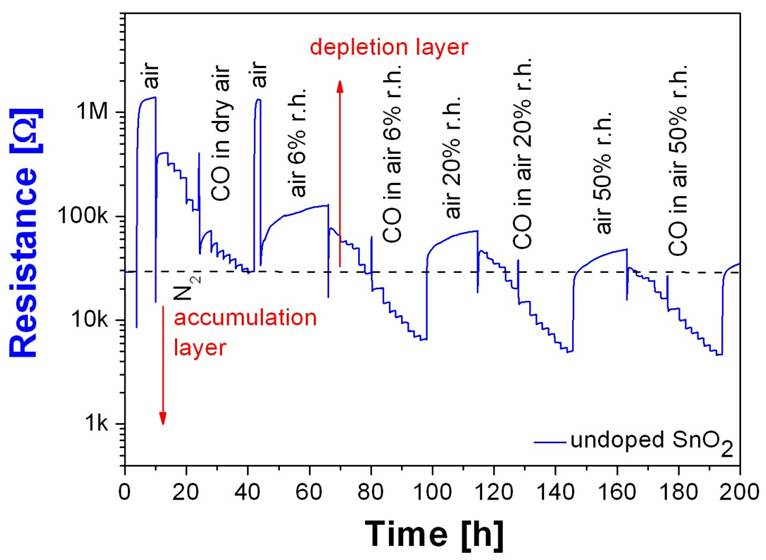
\includegraphics{media/pics/external_plots/nitroline_switch_julia.jpg}
\caption{Nitrogen switch}
\end{figure}

    With the absence of the depletion layer also most simplifications are
not valid anymore. Mainly the validity of the Schottky and Boltzmann
approximation may not be given anymore. Facing those facts the equations
to describe the transduction mechanism for a specific electrical band
configurations needed a more general descriptions, which includes a
depletion and accumulation layer controlled transduction mechanism.

To describe such a semiconductor the set of differential equations is
available in literature. Common simplifications for such problems have
not been valid in the generalized case needed to describe the sensor and
finding an analytically solution exceeded by far my intellectual
capabilities. This is why a I chose to go a different path by
numerically deriving solutions for the problem.

While working in the field of SMOX sensors already some years, I was
used to describe transduction processes by assigning different parts of
an analytical solution to properties of the sensor. With a numerical
solution this is not possible anymore and this was certainly a drawback
of this method. On the other side the relation between intrinsic
properties can still be studied also in detail. By solving the equations
numerically for multiple combinations of the intrinsic property the
resulting dataset can then again be used gain insights about the
fundamental relations of the parameters. Also the comparison of the
numerical results with experimental data might reveals properties, which
can not be measured easily otherwise. Therefore the goal was first to
break the problem of describing a SMOX sensor into smaller discreet
parts and second trying to solve each of it individually.

In the upcoming chapters I will describe the different part and how they
have been simplified, solved individually and combined again. In last
chapter of the thesis, experimental data is compared with the
numerically gained results.

    \hypertarget{numerical-calculation-of-semiconductors-gas-sensors}{%
\section{Numerical calculation of semiconductors gas
sensors}\label{numerical-calculation-of-semiconductors-gas-sensors}}

    \hypertarget{introduction}{%
\subsection{Introduction}\label{introduction}}

To elaborate the modeling of sensing, equations such as the shape
dependent Poisson equation, the electro-neutrality equation and the
geometry dependent electrical current path, must be solved. In most
cases, this is an extensive mathematical effort and therefore, the
numerical computing environments Python will be used to derive numerical
solutions for equations, which cannot be solved analytically, as shown
below. From literature \cite{Rothschild2004b} the grain size dependency
on the charges trapped at the surface has different impact on the
potential and charge distribution inside the grain. For large grains
compared to their Debye length (\(L_D\)), a charge transfer at the
surface may be leave the bulk unaffected. In contrast to large grains,
relative small grains may be affected through the whole grain. This
effect will be the major outcome of the chapter and a graphical
representation is shown at the end.

To understand the influence of the charge transfer at the surface on the
resulting charge density inside the grain is from main importance. With
this knowledge the free charge carrier concentration and a position
dependent resistivity can be defined.

When investigating the total resistance of one grain, the pathway
through the grain plays a major role. The total resistance may vary a
lot based on the an-isotropic resistivity distribution.

    \hypertarget{semiconductor-properties-of-the-smox-grains}{%
\subsection{Semiconductor properties of the SMOX
grains}\label{semiconductor-properties-of-the-smox-grains}}

The advantages of industrialized production techniques are inline with
general advantages of the SMOX-based sensor technologie. Both are:

• upscalable

• highly reproducible

• low cost

Besides the benefits for the industrialization of such a material, also
the resulting morphological are beneficial for a good sensor
performance. The typical spherical grains with a narrow size
distribution result in high surface to volume ration. Besides the high
surface area, the high number of grain-grain contacts have a positive
effect on the sensitivity of the sensor, due to the high number of back
to back Schottky barriers. As described in \cite{Barsan2003}
\cite{Barsan2011a} such barriers are of major importance for the sensing
properties.

In the literature other geometries claim exceptional performances for
multiple other shapes. As from hollow spheres to nano-rods, often the
mechanism which explains the measured increase in performance is not
explained. Since the aim is to gain a fundamental understanding of the
shape influence while staying close to a industrialize material I will
keep the focus in this work on spherical grains, which are commonly used
in commercial products. Nevertheless the techniques described in my work
should be transferable to arbitrary and more complex shapes.

Besides the shape also the defect concentration and stochastic
composition varies a lot with the preparation process. One additional
goal of this thesis is to gain a better understanding about the relation
of these two properties and the sensor performance.

    \hypertarget{choice-of-geometric-model}{%
\subsection{Choice of geometric model}\label{choice-of-geometric-model}}

Most SMOX grains can be well approximated as spherical grains. The
typical diameters of the grains are from 5nm to 200nm. The benefit by
choosing of such a shape with a the rotational symmetry is the reduction
of the complexity for the numerical calculation. Therefore the
approximation of the SMOX particles as spheres was chosen. The second
benefit of choosing materials prepared by rather standardized
preparation routes is the availability of multiple different materials
form varying laboratories around the world. These materials may vary in
sizes and defect concentration but are often similar in shape. This fact
is favorable when the numerical results are compared and validated with
experimental data.

Other available materials with more specialized shapes as hallow spheres
or fibers do exist, but will not be investigated in the research. In the
first place the complex numerical description of such geometries will
increase the calculation duration. Also the limited availability and
variety in parameters as diameter, doping level, band gap, material
composition are not favorable for to check the numerical model with
experimental data.

    \hypertarget{poissons-equation}{%
\subsection{Poisson's equation}\label{poissons-equation}}

Reactions at the surface (see {[}sec:Surface-reactions{]}) result in a
charge transfer between the bulk of a grain and the surface. This
modification of the charge density distribution inside the grain causes
again a change in resistivity . By moving charges to/away from the
surface, electrical potentials through the grain are generated. The
electrical potential at the surface and therefore the work function of
the semiconductor changes (see {[}subsec:Work-function{]}). A detailed
description of work function measurements with the Kelvin Probe method
is described here \cite{Oprea2009a}.

Previous studies have described the direct relation between surface
potential, surface charge and resistance exists. The latter studies
initially define certain approximations which have been adapted and
reasonable for the investigated cases, but do not allow a predictions
outside the boundaries of the pre-assumption. Also the direct impact of
size and geometric on the transduction is not taken fully into
consideration. In order to have a more general model of the SMOX
materials and to include the geometric effects, the charge distribution
has to be solved in a more general way.

Identical to the previous studies the relation between surface potential
and charge distribution has to be solved initially. This relation is
defined by the Poisson-Law:

\begin{align}
\nabla\phi=-\frac{\rho}{\epsilon\epsilon_{0}} \label{eq1}\tag{Poisson}
\end{align}

\(\phi\)=electrical potential, \(\rho\)=free charge density,
\(\epsilon\)=vacuum permittivity, \(\epsilon_{0}\)=relative
permittivity.

It is assume that \(\epsilon\) does not vary inside the grain. The
charge destiny \(\rho\) on the other side is directly influenced by the
charge transfer. Since the transfer of charges to the surface influences
the work function and the energetic position of the conduction band,
\(\rho\) is a function of \(\phi\). \(\phi\) again depends on the
position in the grain. At the surface \(\phi(r=r_{S})\) corresponds to
the surface potential \(\phi_s\), while in the center
\(\phi(r=0)=\phi_b\) may have a different value. The exact shape of
\(\phi(r)\) is gained from solving the Poisson equation \((\ref{eq1})\).

It will be assumed, that the reactions take place a the surface of the
crystal and bulk diffusion will be neglected. Even if there are reports
of oxygen bulk diffusion for certain materials , this is not the general
behavior and does not apply apply for \(SnO_{2}\). Since all surface
sites will be accessible by the gas, the solution of equation: \ref{eq1}
should have a rotational symmetry. In the case of multiple grains with
grain-grain contacts this assumptions needs to be validated again.

In case of an rotational symmetric shape of a SMOX grain, equation
{[}eq:poisson\_eq{]}can be expressed as a ordinary differential equation
of only the radius:

\begin{align}
(\frac{1}{r²})\frac{d}{dr}\frac{r²d\phi(r)}{dr}=-\frac{\rho(r)}{\epsilon\epsilon_{0}}\label{poisson_spherical_1}\tag{Poisson spherical 1}
\end{align}

\hypertarget{charge-density}{%
\subsection{Charge density}\label{charge-density}}

As mentioned, the scope of my work was to investigate the transduction
mechanism. Specially including the phenomena of a switch from a
depletion- to accumulation layer controlled transduction mechanism. The
previously shown conduction mechanism switch an experiment is shown,
where such a switch occurs under application relevant environmental
conditions (50\% r.h. and \textasciitilde3 ppm CO). The findings are
described in detail in \cite{Barsan2015}.

In cases of depletion layer controlled transduction the
Schottky-Approximation was proven to be a effective way to describe and
simplify the Poisson equation. In the case of a accumulation layer the
assumption of a fully depleted space charge layer is not valid anymore.

It should be mentioned, that a common second approximation often used
together with Schottky's approximation is Boltzmann's approximation. The
Boltzmann approximation is valid if the energetic difference between the
energy E and the Fermi level energy \(E_{Fermi}\) is high enough:
\begin{align}
E-E_{Fermi}\gg3k_{B}T
\end{align} In such a case the Fermi-Dirac distribution \(f(E)\) can be
expressed with the Boltzmann distribution b(E):

\begin{align}
f(E)=\frac{1}{exp(\frac{E-E_{Fermi}}{k_{B}T})+1}\xrightarrow{Boltzmann\,Conditions}b(E)=exp(-\frac{(E-E_{Fermi})}{k_{B}T})
\end{align}

Based on the findings, that the flat band situation is reached in
application relevant conditions, the Boltzmann approximation is not
always valid anymore. Operando Kelvin Probe experiments indicate, that
the surface potential may drop up to 1eV below the nitrogen level
\cite{Barsan2015}. The typical difference \(E_{Conduction}-E_{Fermi}\)
is between 50meV and 300meV. It is reasonable to expect, that the
conduction band may even cross the Fermi level and therefore also the
conditions necessary for the Boltzmann approximation do not exist. In
the upcoming calculations I will calculate and show when using the
Boltzmann approximation is legit and when not.

Since the goal of this work is to unify the calculations for all
transduction regions, the Fermi-Dirac distribution, without further
simplification, is used to calculate the charge distributions.

We will begin by rewrite the Fermi-Dirac equation to a suitable format,
which will reflect the the occupation probability at energies relative
to the initial conduction band position \(E_C\):

Ferimi-Dirac: \begin{align}
f(E)=\frac{1}{exp(\frac{E-E_{Fermi}}{k_{B}T})+1}=\frac{1}{exp(\frac{E-E_{C}+E_{C}-E_{Fermi}}{k_{B}T})+1}=\frac{1}{exp(\frac{E_{C}-E_{Fermi}}{k_{B}T})*exp(\frac{E-E_{C}}{k_{B}T})+1}\label{fermi}\tag{Fermi}
\end{align}

The density of states \(g_{E_{C}}\left(E\right)\) with the energy \(E\)
and the conduction band at \(E_{C}\) is given by \cite{Sze2007} as
followed:

\begin{align}
g_{E_{C}}\left(E\right)=\frac{\sqrt{2}}{\Pi^{^{2}}}\frac{\sqrt{E-E_{C}}}{\hbar^{3}}m^{*^{\frac{3}{2}}}=4\Pi*\frac{\left(2*m^{*}\right)^{\frac{3}{2}}}{h^{3}}*\sqrt{E-E_{C}}
\end{align}

The integral of the Fermi occupation probability \(f(E)\)
(\(\ref{fermi}\)) and the density of states \(g_{E_{C}}\left(E\right)\)
results in the the number of charges in the conduction band:

\begin{align}
n\left(E_{C}\right)=\intop_{E_{C}}^{inf}g_{E_{C}}\left(E\right)*f\left(E\right)dE\label{nintegral}\tag{$n(E_C)$}
\end{align}

Typically this equation is simplified to the following form. Such an
analytical equation is useful for further analytical calculations but is
not necessary for our numerical approach:

\begin{align}
n(E_{C})=N_{C}exp\left(\frac{E_{F}-E_{C}}{k_{B}T}\right)
\end{align}

with
\(N_{C}=2\left(\frac{2\Pi m_{e}^{*}k_{B}T}{h²}\right)^{\frac{3}{2}}\),
the effective density of states in the conduction band. It is worth-wise
to mention, that this simplification is only valid if also the Boltzmann
approximation is valid.

Equation \ref{nintegral} is solved numerically and compared with the
results obtained with the common approximations. \(m_{e}^{*}=0.3m_{e}\)
for \(SnO_{2}\) was chosen based on \cite{Batzill2005}.

Above a operation temperature of 300°C, all donors are ionized and
available as free charge carriers in the conduction band
\cite{Barsan2015}. If some of those electrons are trapped at the surface
due to surface reaction, a positive charge remains localized in the
crystal at the donors position. Additionally the energetic position of
the conduction band increases with electron trapped at the surface. Out
of the combination of conduction band shift \(E=E_{C}-E_{C_{b}}\) and
equation \ref{nintegral}, one can calculate the free charge carrier
density \(\rho\) from Poisson's equation.

In the case of an unaffected bulk, \(n(E_{C_{b}})\equiv n_{b}\) is the
density of electrons in the conduction band. In case of a charge
transfer to/from the surface, the number of electrons in the conduction
band will change. The relation between the density of charges in the
conduction band \(n(E_{C})\) and the shifted, new energetic position of
the conduction band \(E_{C}\) is fixed by equation \ref{nintegral}. The
difference between \(n_{b}\) and \(n(E_{C})\) is the density of the
positive, ionized donors remaining in the crystal. Those remaining
donors are the cause of the electrical screening of the surface
potential. The decay of the energetic conduction band position from the
surface energy level back to the `bulk position' depends directly on
that number. With this relation a energy dependent charge density can be
formulated as followed:

\begin{align}
\frac{\rho(E)}{e}=n(E_{C_b})-n(E) = n_{b}-n(E)
\end{align}

Equation \ref{poisson_spherical_1} becomes then:

\begin{align}
\left(\frac{1}{r²}\right)\frac{d}{dr}\frac{r²d\phi}{dr}=-\frac{\rho\left(E\left(r\right)\right)}{\epsilon\epsilon_{0}}=-\frac{e\left(n\left(E_{C_{b}}\right)-n\left(E\right)\right)}{\epsilon\epsilon_{0}}=-\frac{e\left(n_{b}-n\left(E\right)\right)}{\epsilon\epsilon_{0}}\label{poisson_spherical}\tag{Poisson spherical 2}
\end{align}

With \(E=V*e=(\Phi_{0}-\Phi)*e\)

``In discussions of semiconductos, it is useful to define a''band
bending" function \(V\) such that \(eV\) is related to the potential
energy of an electron''\cite{S.RoyMorrison1977}::

\(V=\phi_{b}-\phi,\;E=V*e\)

With this relation equation (\ref{poisson_spherical}) becomes:

\begin{align}
\left(\frac{1}{r²}\right)\frac{d}{dr}\frac{r²dV}{dr}=\frac{e\left(n_{b}-n\left(E\right)\right)}{\epsilon\epsilon_{0}}\label{poisson_spher_v}\tag{Poisson spherical (V)}
\end{align}

With this relation is is possible to calculate how the potential at the
surface is electrically screen by the remaining positive charges inside
the grain. An important parameter for such calculations is the Debye
length. In cases where the Boltzmann approximation is valid, the Debye
length can be approximated with the following formula. In this case the
given length is the distance needed to screen a potential \(V\) until
its value reaches \(\frac{V}{e}\). Even if the Boltzmann approximation
may not be valid in all the cases to be calculated, the Debye length
will still be used as material specific property.

\begin{align}
L_{D}=\sqrt{\frac{\epsilon\epsilon_{0}k_{B}T}{n_{b}e^{2}}}
\end{align}

With the definition of the Debye length all relevant variables of the
calculation can be express without physical units as ratios of material
specific parameters.

\begin{itemize}
\item
  The distance inside the grain r is expressed in units of the Debye
  length \(L_{D}\) :

  \(r^{*}=\frac{r}{L_{D}}, \frac{dr^{*}}{dr}=\frac{1}{L_{D}}\longrightarrow dr=dr^{*}*L_{D}\)
\item
  The position of the conduction band inside the grain in units of the
  \(\frac{k_{B}T}{e}\):

  \(V^{*}=\frac{e}{k_{B}T}*V, \frac{dV^{*}}{dV}=\frac{e}{k_{B}T}\longrightarrow dV=dV^{*}*\frac{k_{B}T}{e}\)
\item
  And the number of free charge carries in units of the intrinsic number
  of charges \(n_b\):

  \(n^{*}(V^{*})=\frac{n(V)}{n_{b}}\)
\end{itemize}

By substituting those unit-less parameters in equation
(\ref{poisson_spher_v}), one obtains the a unit-less Poisson equation
suitable for the numerical calculations:

\begin{align}
\frac{1}{r^{*2}}\frac{d}{dr^{*}}{r^{*}}^{2}\frac{dV^{*}}{dr^{*}}=1-n^{*}(V^{*})\label{poisson_no_units}\tag{Unitless Poisson equation}
\end{align}

This step of substituting the equation with unit less parameters is not
obligatory for the the numerical calculations. As I will show in the
next part of the thesis, the numerical calculation is also be possible
with the initial spherical Poisson equation (\ref{poisson_spher_v}).
Therefore the material specific parameters need to be given to the
algorithm. The downside would be, that for every new material with any
parameter changing, the calculation would need to be redone. The benefit
of the latter derived equation is that it is valid for multiple
combinations of intrinsic parameters. The solution would only depend on
three parameters:

\begin{itemize}
\tightlist
\item
  Grainsize \(R\) in units of \(L_{D}\)
\item
  Temperature \(T\) as in \(\frac{k_{B}T}{e}\)
\item
  The doping level of the semiconductor described with \(n_b\)
\end{itemize}

The advantage of the numerical approch is now, that for typical values
of these parameters the solution are computed and used for further
understanding of their influence on sensing with SMOX material. Typical
values of the relevant parameters are:

\begin{itemize}
\tightlist
\item
  Typical grainsizes reach from 0.1 to 100 \(L_D\)
\item
  Typical temperatures are in the range of 100°C to 400°C
\item
  The doping level \(n_b\) range from \(10^{20}\frac{1}{m^3}\) to
  \(10^{25}\frac{1}{m^3}\)
\end{itemize}

This indicates just the typical materials, but solutions for other
parameters are alos possible. For the scope of my work I will
nevertheless concentrate on the gives ranges.

\hypertarget{poisson-equation-as-system-of-odes}{%
\subsection{Poisson equation as system of
ODEs}\label{poisson-equation-as-system-of-odes}}

The Python SciPy package (\cite{Jones}, \cite{Virtanen2020} ) will now
be used to numerically solve the derived equations. The ``odesolvers''
of SciPy are able to solve first order ODEs, or systems of first order
ODES. To solve a second order ODE, if must first by converted by changes
of variables to a system of first order ODES.

Equation (\ref{poisson_no_units}) is an ODE of second order, so it it
needs to be express as a system of first order ODES.

Practically a functions needs to be defined, which gets as input an list
of functions and returns an list of the derived functions:

\begin{align}
derive\_func\left(V^{*},\frac{dV^{*}}{dr^{*}}\right)\longrightarrow\frac{dV^{*}}{dr^{*}},\frac{d^2V^{*}}{dr^{*2}}
\end{align}

The second input term \(\frac{dV^{*}}{dr^{*}}\) corresponds already to
the first output term. So no special work needs to be done here. But
also the second output parameter can be calculated with the given input
parameters by using (\ref{poisson_no_units}).

\begin{align}
\frac{1}{r^{*2}}\frac{d}{dr^{*}}{r^{*}}^{2}\frac{dV^{*}}{dr^{*}}=1-n^{*}(V^{*})=\frac{2r^{*}}{r^{*2}}\frac{dV^{*}}{dr^{*}}+\frac{r^{*2}}{r^{*2}}\frac{d²V^{*}}{dr^{*2}}=\frac{2}{r^{*}}\frac{dV^{*}}{dr^{*}}+\frac{d²V^{*}}{dr^{*2}}=1-n^{*}(V^{*}) 
\end{align}

\begin{align}
\frac{d²V^{*}}{dr^{*2}}=1-n^{*}(V^{*})-\frac{2}{r^{*}}\frac{dV^{*}}{dr^{*}}\label{second_derivative}\tag{Second derivative}
\end{align}

The odesolver needs beside the derive-function additional parameters.
Namely a set of initial start values for \(V^{*}\) and
\(\frac{dV^{*}}{dr^{*}}\) and boundaries in between the solver should
calculate the solution. Since we first want to calculate the shape of
the conduction band resulting from different surface potentials
\(V^{*}_{Surface}\), the initial parameter \(V^{*}{}_{init}\) is already
defined as \(V^{*}_{Surface}\). Also the boundaries should be the full
grain, so r\^{}* is between 0 and the grain radius \(R^*\). Only the
\(\frac{dV^{*}}{dr^{*}}|_{init}\) can not directly be defined.
Nevertheless a the correct solution of the differential equation can
still be found. This will be done by solving the equation for multiple
initial values of \(\frac{dV^{*}}{dr^{*}}|_{init}\) and ``picking'' the
right solution. This step will be described in detail in a later part of
this chapter.

\(odesolver(derive\_func,[V^{*}{}_{init},\frac{dV^{*}}{dr^{*}}_{init}],r)\longrightarrow V^{*}(r^{*}),\frac{dV^{*}}{dr*}(r*)\)

    \hypertarget{constants}{%
\subsection{Constants}\label{constants}}

For the numerical calculations I will need to use some constants to
refer to. To structure this notebook it is favorable to concentrate the
definition at a single point and refer always back to this definition.
This reduces the potential error of typos when using some constants over
and over again.

One way to generate a global object which groups the relevant
information together and allows to access them easily are classes. Such
classes do not only store the relevant information but offer also some
useful functionalities related to the stored information.

In the following code block, the class is defined with the statement
\texttt{class}. What the follows the \texttt{class} statement is the
name of the class. By convention class names start with a capital
letter. Inside the \texttt{class} initially one function called
\texttt{\_\_init\_\_} is defined with the
\texttt{def\ \_\_init\_\_(self):} statement. This special function is
always automatically executed when an instance of the class is created.
Here I define some constants, which are relevant for course of this
thesis. I also add some useful functions, e.g.~the conversion from
Celsius to Kelvin and vise versa. Such functions will be of mayor
importance when doing the knowledge transfer gained in the
`semiconductor regime' (Kelvin is the useful scale here) to application
relevant conditions (where Celsius is the usual temperature scale).

    \begin{tcolorbox}[breakable, size=fbox, boxrule=1pt, pad at break*=1mm,colback=cellbackground, colframe=cellborder]
\prompt{In}{incolor}{1}{\boxspacing}
\begin{Verbatim}[commandchars=\\\{\}]
\PY{k+kn}{from} \PY{n+nn}{scipy} \PY{k+kn}{import} \PY{n}{constants} \PY{k}{as} \PY{n}{sciConst}
\PY{k}{class} \PY{n+nc}{Constant}\PY{p}{:}
    \PY{k}{def} \PY{n+nf+fm}{\PYZus{}\PYZus{}init\PYZus{}\PYZus{}}\PY{p}{(}\PY{n+nb+bp}{self}\PY{p}{)}\PY{p}{:}
        \PY{n+nb+bp}{self}\PY{o}{.}\PY{n}{K0} \PY{o}{=} \PY{n}{sciConst}\PY{o}{.}\PY{n}{convert\PYZus{}temperature}\PY{p}{(}\PY{l+m+mi}{0}\PY{p}{,}\PY{l+s+s1}{\PYZsq{}}\PY{l+s+s1}{C}\PY{l+s+s1}{\PYZsq{}}\PY{p}{,}\PY{l+s+s1}{\PYZsq{}}\PY{l+s+s1}{K}\PY{l+s+s1}{\PYZsq{}}\PY{p}{)}
        \PY{n+nb+bp}{self}\PY{o}{.}\PY{n}{kB}\PY{o}{=}\PY{n}{sciConst}\PY{o}{.}\PY{n}{k}
        \PY{n+nb+bp}{self}\PY{o}{.}\PY{n}{EPSILON\PYZus{}0} \PY{o}{=} \PY{n}{sciConst}\PY{o}{.}\PY{n}{epsilon\PYZus{}0}
        \PY{n+nb+bp}{self}\PY{o}{.}\PY{n}{E\PYZus{}CHARGE} \PY{o}{=} \PY{n}{sciConst}\PY{o}{.}\PY{n}{elementary\PYZus{}charge}
        \PY{n+nb+bp}{self}\PY{o}{.}\PY{n}{h} \PY{o}{=} \PY{n}{sciConst}\PY{o}{.}\PY{n}{h}
        \PY{n+nb+bp}{self}\PY{o}{.}\PY{n}{MASS\PYZus{}E} \PY{o}{=} \PY{n}{sciConst}\PY{o}{.}\PY{n}{electron\PYZus{}mass}
        \PY{n+nb+bp}{self}\PY{o}{.}\PY{n}{NA}\PY{o}{=} \PY{n}{sciConst}\PY{o}{.}\PY{n}{N\PYZus{}A}
        \PY{n+nb+bp}{self}\PY{o}{.}\PY{n}{VOL\PYZus{}mol} \PY{o}{=} \PY{l+m+mf}{22.4}
        \PY{n+nb+bp}{self}\PY{o}{.}\PY{n}{mole\PYZus{}per\PYZus{}l} \PY{o}{=} \PY{n+nb+bp}{self}\PY{o}{.}\PY{n}{NA}\PY{o}{/}\PY{n+nb+bp}{self}\PY{o}{.}\PY{n}{VOL\PYZus{}mol}
        
    \PY{k}{def} \PY{n+nf}{K\PYZus{}to\PYZus{}C}\PY{p}{(}\PY{n+nb+bp}{self}\PY{p}{,} \PY{n}{K}\PY{p}{)}\PY{p}{:}
        \PY{k}{return} \PY{n}{sciConst}\PY{o}{.}\PY{n}{convert\PYZus{}temperature}\PY{p}{(}\PY{n}{K}\PY{p}{,} \PY{l+s+s1}{\PYZsq{}}\PY{l+s+s1}{K}\PY{l+s+s1}{\PYZsq{}}\PY{p}{,} \PY{l+s+s1}{\PYZsq{}}\PY{l+s+s1}{C}\PY{l+s+s1}{\PYZsq{}}\PY{p}{)}

    \PY{k}{def} \PY{n+nf}{C\PYZus{}to\PYZus{}K}\PY{p}{(}\PY{n+nb+bp}{self}\PY{p}{,} \PY{n}{C}\PY{p}{)}\PY{p}{:}
        \PY{k}{return} \PY{n}{sciConst}\PY{o}{.}\PY{n}{convert\PYZus{}temperature}\PY{p}{(}\PY{n}{C}\PY{p}{,} \PY{l+s+s1}{\PYZsq{}}\PY{l+s+s1}{C}\PY{l+s+s1}{\PYZsq{}}\PY{p}{,} \PY{l+s+s1}{\PYZsq{}}\PY{l+s+s1}{K}\PY{l+s+s1}{\PYZsq{}}\PY{p}{)}
    
    \PY{k}{def} \PY{n+nf}{eV\PYZus{}to\PYZus{}J}\PY{p}{(}\PY{n+nb+bp}{self}\PY{p}{,}\PY{n}{eV}\PY{p}{)}\PY{p}{:}
        \PY{k}{return} \PY{n}{eV}\PY{o}{*}\PY{n+nb+bp}{self}\PY{o}{.}\PY{n}{E\PYZus{}CHARGE}
    
    \PY{k}{def} \PY{n+nf}{J\PYZus{}to\PYZus{}eV}\PY{p}{(}\PY{n+nb+bp}{self}\PY{p}{,}\PY{n}{J}\PY{p}{)}\PY{p}{:}
        \PY{k}{return} \PY{n}{J}\PY{o}{/}\PY{n+nb+bp}{self}\PY{o}{.}\PY{n}{E\PYZus{}CHARGE}
    
    
\PY{n}{CONST} \PY{o}{=} \PY{n}{Constant}\PY{p}{(}\PY{p}{)}
\end{Verbatim}
\end{tcolorbox}

    \hypertarget{materials}{%
\subsection{Materials}\label{materials}}

    Once the basic constants are defined, creating also a simplified
numerical representation of the investigated semiconducting material. As
explained in the theoretical section, the charge distribution \(n\),
depends on the position of the conduction band and is the result from
solving an integral. For our calculations this integral will be solved
numerically. So before all the relevant parameters of the SMOX material
can be defined, a short introduction into solving integrals with Python
is useful. Again start with setting up a numerical python lab, which
will output all results ``inline'' with this document. As shown in the
introduction this is done by using the magic command
\texttt{\%pylab\ inline}

    \begin{tcolorbox}[breakable, size=fbox, boxrule=1pt, pad at break*=1mm,colback=cellbackground, colframe=cellborder]
\prompt{In}{incolor}{4}{\boxspacing}
\begin{Verbatim}[commandchars=\\\{\}]
\PY{o}{\PYZpc{}}\PY{k}{pylab} inline
\end{Verbatim}
\end{tcolorbox}

    \begin{Verbatim}[commandchars=\\\{\}]
Populating the interactive namespace from numpy and matplotlib
    \end{Verbatim}

    \begin{Verbatim}[commandchars=\\\{\}]
/usr/lib/python3.8/site-packages/IPython/core/magics/pylab.py:159: UserWarning:
pylab import has clobbered these variables: ['f']
`\%matplotlib` prevents importing * from pylab and numpy
  warn("pylab import has clobbered these variables: \%s"  \% clobbered +
    \end{Verbatim}

    \hypertarget{solving-integrals-numerically}{%
\subsubsection{Solving integrals
numerically}\label{solving-integrals-numerically}}

\hypertarget{introduction}{%
\paragraph{Introduction}\label{introduction}}

Many observables in nature can be predicted with the solution an
integral of a certain function. In this section I will make a short
excursion on how to solve integrals numerically.

From my experience, many students and researches excellently trained to
define the set of equations describing their problems mathematically.
Second, also the evaluation of the individual equations with multiple
variables imposes (in most cases) no problem. And third, it is also part
of the common knowledge, that the integral of any function is equivalent
to the area below the curve. A college of mine once told me, that she
learn calculating the integral in school by: 1. drawing the function for
multiple points on a paper 2. combine them with a line 3. count the
squares below the curve

Nothing else is done, when solving integrals numerically with Python.
And we will see, that this method is quite accurate.

On the other side solving an integral analytically requires in many
cases advanced mathematical skills and often
approximation/simplifications are introduces to be able to solve the
problem. Those tasks are often hard to master for many people (including
me) and the simplifications often reduce the solution to specific
boundary conditions (as for example the Boltzmann approximation).

As mentioned solving integrals numerically is fairly easy, even if one
might not feel very comfortable with counting squares. But even if
counting is not an option, there are modern tools to solve this task
very efficiently! If haven't been introduced yet, here they come!

So if the elements to be integrated can evaluated for each point between
the boundaries of the integral, not much is in the way to solve the
integral numerically. Here a simple example of solving:

\begin{align}
\intop_{3}^{5}x{{}^5}dx
\end{align}

The analytical solution solution is: \begin{align}
\left[1/6x^6\right]_{3}^{5}=1/6*5^6-1/6*3^6\backsimeq2482.67
\end{align}

    \hypertarget{the-quad-function}{%
\paragraph{\texorpdfstring{The \texttt{quad}
function}{The quad function}}\label{the-quad-function}}

The \texttt{quad} function from the \texttt{scipy.integrate} package
will be used to integrate the given function. The \texttt{quad} needs as
comma separated inputs the 1. function to integrate 2. the lower
integration boundary 3. the upper integration boundary

The help file of \texttt{quad} says: \textgreater Integrate func from
\texttt{a} to \texttt{b} (possibly infinite interval) using a technique
from the Fortran library QUADPACK.

This
\href{https://docs.scipy.org/doc/scipy/reference/generated/scipy.integrate.quad.html}{description}
reveals, that the Fortran library QUADPACK is used in the background. So
nothing new is shown here from the ``scientific'' point of view. I'd
rather like to point out, how easy this can be applied in a Jupyter
notebook. From discussion with colleagues I know, that the biggest
challenge is how to technically implement the numerical solving
algorithm in Python. So here it comes:

    \begin{tcolorbox}[breakable, size=fbox, boxrule=1pt, pad at break*=1mm,colback=cellbackground, colframe=cellborder]
\prompt{In}{incolor}{5}{\boxspacing}
\begin{Verbatim}[commandchars=\\\{\}]
\PY{k+kn}{from} \PY{n+nn}{scipy}\PY{n+nn}{.}\PY{n+nn}{integrate} \PY{k+kn}{import} \PY{n}{quad}

\PY{k}{def} \PY{n+nf}{f}\PY{p}{(}\PY{n}{x}\PY{p}{)}\PY{p}{:}
    \PY{c+c1}{\PYZsh{} return x to the power 5}
    \PY{k}{return} \PY{n}{x}\PY{o}{*}\PY{o}{*}\PY{l+m+mi}{5}

\PY{c+c1}{\PYZsh{}numerical solution}
\PY{n}{num\PYZus{}sol}\PY{p}{,} \PY{n}{num\PYZus{}error} \PY{o}{=} \PY{n}{quad}\PY{p}{(}\PY{n}{f}\PY{p}{,}\PY{l+m+mi}{3}\PY{p}{,}\PY{l+m+mi}{5}\PY{p}{)}

\PY{c+c1}{\PYZsh{}analytical solution}
\PY{n}{ana\PYZus{}sol} \PY{o}{=} \PY{l+m+mi}{1}\PY{o}{/}\PY{l+m+mi}{6}\PY{o}{*}\PY{p}{(}\PY{l+m+mi}{5}\PY{o}{*}\PY{o}{*}\PY{l+m+mi}{6}\PY{o}{\PYZhy{}}\PY{l+m+mi}{3}\PY{o}{*}\PY{o}{*}\PY{l+m+mi}{6}\PY{p}{)}

\PY{n+nb}{print}\PY{p}{(}\PY{l+s+sa}{f}\PY{l+s+s1}{\PYZsq{}}\PY{l+s+s1}{Numerical solution: }\PY{l+s+si}{\PYZob{}num\PYZus{}sol:.2f\PYZcb{}}\PY{l+s+s1}{ +\PYZhy{} }\PY{l+s+si}{\PYZob{}num\PYZus{}error:.2f\PYZcb{}}\PY{l+s+s1}{\PYZsq{}}\PY{p}{)}
\PY{n+nb}{print}\PY{p}{(}\PY{l+s+sa}{f}\PY{l+s+s1}{\PYZsq{}}\PY{l+s+s1}{Analytical solution: }\PY{l+s+si}{\PYZob{}ana\PYZus{}sol:.2f\PYZcb{}}\PY{l+s+s1}{\PYZsq{}}\PY{p}{)}
\end{Verbatim}
\end{tcolorbox}

    \begin{Verbatim}[commandchars=\\\{\}]
Numerical solution: 2482.67 +- 0.00
Analytical solution: 2482.67
    \end{Verbatim}

    In this case, the numerical and the analytical solution result in the
same results. It is worth to mention, that \texttt{quad} not only
returns the actual value of the integral, but also
\href{https://docs.scipy.org/doc/scipy/reference/generated/scipy.integrate.quad.html}{``an
estimate of the absolute error in the result.''}.

How about a more complex problem? Let's look at the ``Normal
distribution'': \begin{align}
f(x)=\frac{1}{\sqrt{2\Pi}}*e^{-\frac{x²}{2}}
\end{align} Since the probability distribution is normalized the
integral from \(-\infty\) to \(\infty\) is 1: \begin{align}
\intop_{-\infty}^{\infty}f(x)dx=1
\end{align} The analytical solution of this integral is already a rather
advanced task, but still doable. The numerical results are obtained in
the following cell.

    \begin{tcolorbox}[breakable, size=fbox, boxrule=1pt, pad at break*=1mm,colback=cellbackground, colframe=cellborder]
\prompt{In}{incolor}{6}{\boxspacing}
\begin{Verbatim}[commandchars=\\\{\}]
\PY{k}{def} \PY{n+nf}{f}\PY{p}{(}\PY{n}{x}\PY{p}{)}\PY{p}{:}
    \PY{k}{return} \PY{l+m+mi}{1}\PY{o}{/}\PY{p}{(}\PY{l+m+mi}{2}\PY{o}{*}\PY{n}{pi}\PY{p}{)}\PY{o}{*}\PY{o}{*}\PY{l+m+mf}{0.5}\PY{o}{*}\PY{n}{e}\PY{o}{*}\PY{o}{*}\PY{p}{(}\PY{o}{\PYZhy{}}\PY{p}{(}\PY{n}{x}\PY{o}{*}\PY{o}{*}\PY{l+m+mi}{2}\PY{o}{/}\PY{l+m+mi}{2}\PY{p}{)}\PY{p}{)}

\PY{n}{num\PYZus{}sol}\PY{p}{,} \PY{n}{num\PYZus{}error} \PY{o}{=} \PY{n}{quad}\PY{p}{(}\PY{n}{f}\PY{p}{,} \PY{o}{\PYZhy{}}\PY{n}{np}\PY{o}{.}\PY{n}{inf}\PY{p}{,}\PY{n}{np}\PY{o}{.}\PY{n}{inf}\PY{p}{)}
\PY{n}{ana\PYZus{}sol} \PY{o}{=} \PY{l+m+mi}{1}

\PY{n}{num\PYZus{}sol}\PY{p}{,} \PY{n}{num\PYZus{}error} \PY{o}{=} \PY{n}{quad}\PY{p}{(}\PY{n}{f}\PY{p}{,} \PY{o}{\PYZhy{}}\PY{n}{inf}\PY{p}{,}\PY{n}{inf}\PY{p}{)}
\PY{n}{ana\PYZus{}sol} \PY{o}{=} \PY{l+m+mi}{1}

\PY{n+nb}{print}\PY{p}{(}\PY{l+s+sa}{f}\PY{l+s+s1}{\PYZsq{}}\PY{l+s+s1}{Numerical solution: }\PY{l+s+si}{\PYZob{}num\PYZus{}sol:.12f\PYZcb{}}\PY{l+s+s1}{ +\PYZhy{} }\PY{l+s+si}{\PYZob{}num\PYZus{}error:.12f\PYZcb{}}\PY{l+s+s1}{\PYZsq{}}\PY{p}{)}
\PY{n+nb}{print}\PY{p}{(}\PY{l+s+sa}{f}\PY{l+s+s1}{\PYZsq{}}\PY{l+s+s1}{Analytical solution: }\PY{l+s+si}{\PYZob{}ana\PYZus{}sol:.12f\PYZcb{}}\PY{l+s+s1}{\PYZsq{}}\PY{p}{)}
\end{Verbatim}
\end{tcolorbox}

    \begin{Verbatim}[commandchars=\\\{\}]
Numerical solution: 1.000000000000 +- 0.000000010178
Analytical solution: 1.000000000000
    \end{Verbatim}

    Also here a numerical solution is in line with the expected result from
the analytic solution, if we can accept and error of 10ppb. In may cases
such a small error is acceptable.

These two examples cover functions, where a analytical solution is
known. In the following parts of this thesis, many analytical solutions
are not known. In this case the shortcut of using a numerical solution
instead of relaying on the exact solution is reasonable.

\hypertarget{side-note}{%
\paragraph{Side-Note:}\label{side-note}}

The \texttt{print()} statement is used to add the results in the output
of the notebook. The \texttt{print} command requires a text
\emph{string} between its parenthesis. In Python a \emph{string}
consists of multiple characters between quotation marks:
e.g.~\texttt{\textquotesingle{}L3TT3R5\textquotesingle{}}. Additionally
another rather new feature of Python is used here. This feature is
called \emph{formatted strings}. \emph{Formatted strings} are
constructed with an \texttt{f} in front of the \emph{string}:
\texttt{f\textquotesingle{}L3TT3R5\textquotesingle{}}.

For formatted strings variables inside curly parenthesis are then
replaced with their string representation. The formatting of the
representation may be given after \texttt{:}. For example \texttt{.12f}
tells the formatter to represent the variable as a float with 12 digits
after the decimal separator. When reading this as an interactive
notebook, feels free to modify the formatting statement and check the
result.

    \hypertarget{numerical-description-of-the-semiconductor}{%
\subsubsection{Numerical description of the
semiconductor}\label{numerical-description-of-the-semiconductor}}

    \hypertarget{helper-functions-for-semiconductor-calculations}{%
\paragraph{Helper functions for semiconductor
calculations}\label{helper-functions-for-semiconductor-calculations}}

Dr.~Michael Hübner (page 50) derived in his thesis a way to approximate
the energetic difference between the the level of the Fermi-Level and
the conduction band (in a flat band situation) depending of the
temperature \(T\), concentration of defects in the bulk of the grain
\(N_D\) and the effective mass of electrons inside the semiconductor
\(m_e^*\). \(N_D\) is difficult to measure experimentally so this thesis
will initially start with reasonable values found in literature.

For a the later deep analysis \(N_D\) may be screen for the analysis of
their influence on the overall performance of a sensing material.

Based on Michael Hübners work it is possible to derive a value for the
energetic distance between Fermi level and conduction band
\(\Delta E_{CF} = E_C-E_F,\).

Since the energetic distance from the Fermi level mainly defines the
occupation probability of the states in the conduction band, this term
is of major importance. It should be pointed out, that the calculation
in the thesis are based special assumption only valid for \(SnO_2\). The
definition is translated into a Python algorithm and used as an starting
point for further calculations. Besides this function also two other
``helper functions'' are defined which will be used at multiple places
in the upcoming calculations.

    \begin{tcolorbox}[breakable, size=fbox, boxrule=1pt, pad at break*=1mm,colback=cellbackground, colframe=cellborder]
\prompt{In}{incolor}{7}{\boxspacing}
\begin{Verbatim}[commandchars=\\\{\}]
\PY{k+kn}{import} \PY{n+nn}{scipy} 
\PY{k}{def} \PY{n+nf}{calc\PYZus{}kT}\PY{p}{(}\PY{n}{T\PYZus{}C}\PY{p}{)}\PY{p}{:}
    \PY{l+s+sd}{\PYZdq{}\PYZdq{}\PYZdq{}}
\PY{l+s+sd}{    Calculate the kT value for a temp. in °C}
\PY{l+s+sd}{    T\PYZus{}C = Temp in °C}
\PY{l+s+sd}{    \PYZdq{}\PYZdq{}\PYZdq{}}
    
    \PY{n}{kT} \PY{o}{=} \PY{n}{CONST}\PY{o}{.}\PY{n}{kB}\PY{o}{*}\PY{p}{(}\PY{n}{CONST}\PY{o}{.}\PY{n}{C\PYZus{}to\PYZus{}K}\PY{p}{(}\PY{n}{T\PYZus{}C}\PY{p}{)}\PY{p}{)}
    \PY{k}{return} \PY{n}{kT}

\PY{k}{def} \PY{n+nf}{calc\PYZus{}eff\PYZus{}density\PYZus{}of\PYZus{}states}\PY{p}{(}\PY{n}{T\PYZus{}C}\PY{p}{,}\PY{n}{mass\PYZus{}e\PYZus{}eff\PYZus{}factor}\PY{p}{)}\PY{p}{:}
    \PY{l+s+sd}{\PYZdq{}\PYZdq{}\PYZdq{}}
\PY{l+s+sd}{    Calculate the eff. densitiy of states in the conduction band}
\PY{l+s+sd}{    T\PYZus{}C = Temp in °C}
\PY{l+s+sd}{    mass\PYZus{}e\PYZus{}eff\PYZus{}factor = material specific factor to calculate the effective mass}
\PY{l+s+sd}{                        from the electron mass}
\PY{l+s+sd}{    \PYZdq{}\PYZdq{}\PYZdq{}}
    
    \PY{n}{kT} \PY{o}{=} \PY{n}{calc\PYZus{}kT}\PY{p}{(}\PY{n}{T\PYZus{}C}\PY{p}{)}
    \PY{n}{MASS\PYZus{}E\PYZus{}EFF} \PY{o}{=} \PY{n}{mass\PYZus{}e\PYZus{}eff\PYZus{}factor}\PY{o}{*}\PY{n}{CONST}\PY{o}{.}\PY{n}{MASS\PYZus{}E}
    \PY{n}{NC} \PY{o}{=} \PY{l+m+mi}{2}\PY{o}{*}\PY{p}{(}\PY{l+m+mi}{2}\PY{o}{*}\PY{n}{np}\PY{o}{.}\PY{n}{pi}\PY{o}{*}\PY{n}{MASS\PYZus{}E\PYZus{}EFF}\PY{o}{*}\PY{n}{kT}\PY{o}{/}\PY{p}{(}\PY{n}{CONST}\PY{o}{.}\PY{n}{h}\PY{o}{*}\PY{o}{*}\PY{l+m+mi}{2}\PY{p}{)}\PY{p}{)}\PY{o}{*}\PY{o}{*}\PY{p}{(}\PY{l+m+mf}{3.0}\PY{o}{/}\PY{l+m+mf}{2.0}\PY{p}{)}
    \PY{k}{return} \PY{n}{NC}

\PY{k}{def} \PY{n+nf}{calc\PYZus{}EDCF\PYZus{}by\PYZus{}temp}\PY{p}{(}\PY{n}{T\PYZus{}C}\PY{p}{,} \PY{n}{ND}\PY{p}{,}\PY{n}{mass\PYZus{}e\PYZus{}eff\PYZus{}factor}\PY{p}{)}\PY{p}{:}
    \PY{l+s+sd}{\PYZdq{}\PYZdq{}\PYZdq{}}
\PY{l+s+sd}{    T\PYZus{}C = Temperature in °C}
\PY{l+s+sd}{    }
\PY{l+s+sd}{    ND = number of donors per m³}
\PY{l+s+sd}{    ND = 9e21 \PYZsh{} 9*10**15 cm**3 Mich Thesis Seite 50}
\PY{l+s+sd}{    }
\PY{l+s+sd}{    mass\PYZus{}e\PYZus{}eff\PYZus{}factor = material specific factor to calculate the effective mass}
\PY{l+s+sd}{                        from the electron mass}
\PY{l+s+sd}{    \PYZdq{}\PYZdq{}\PYZdq{}}
    
        
    \PY{n}{kT} \PY{o}{=} \PY{n}{calc\PYZus{}kT}\PY{p}{(}\PY{n}{T\PYZus{}C}\PY{p}{)}
    
    \PY{n}{NC} \PY{o}{=} \PY{n}{calc\PYZus{}eff\PYZus{}density\PYZus{}of\PYZus{}states}\PY{p}{(}\PY{n}{T\PYZus{}C}\PY{p}{,}\PY{n}{mass\PYZus{}e\PYZus{}eff\PYZus{}factor}\PY{p}{)}
    
    \PY{n}{ED1C\PYZus{}eV} \PY{o}{=} \PY{l+m+mf}{0.034}
    \PY{n}{ED2C\PYZus{}eV} \PY{o}{=} \PY{l+m+mf}{0.140}
    
    \PY{n}{a} \PY{o}{=} \PY{n}{np}\PY{o}{.}\PY{n}{exp}\PY{p}{(}\PY{n}{CONST}\PY{o}{.}\PY{n}{eV\PYZus{}to\PYZus{}J}\PY{p}{(}\PY{n}{ED1C\PYZus{}eV}\PY{p}{)}\PY{o}{/}\PY{n}{kT}\PY{p}{)}
    \PY{n}{b} \PY{o}{=} \PY{n}{np}\PY{o}{.}\PY{n}{exp}\PY{p}{(}\PY{n}{CONST}\PY{o}{.}\PY{n}{eV\PYZus{}to\PYZus{}J}\PY{p}{(}\PY{n}{ED2C\PYZus{}eV}\PY{p}{)}\PY{o}{/}\PY{n}{kT}\PY{p}{)}
    \PY{n}{t3} \PY{o}{=} \PY{l+m+mf}{1.0}
    \PY{n}{t2} \PY{o}{=} \PY{p}{(}\PY{l+m+mf}{1.0}\PY{o}{/}\PY{n}{b}\PY{o}{\PYZhy{}}\PY{l+m+mf}{0.5}\PY{o}{*}\PY{n}{NC}\PY{o}{/}\PY{n}{ND}\PY{p}{)}
    \PY{n}{t1} \PY{o}{=} \PY{o}{\PYZhy{}}\PY{l+m+mf}{1.0}\PY{o}{/}\PY{n}{b}\PY{o}{*}\PY{n}{NC}\PY{o}{/}\PY{n}{ND}
    \PY{n}{c} \PY{o}{=} \PY{o}{\PYZhy{}}\PY{l+m+mf}{1.0}\PY{o}{/}\PY{p}{(}\PY{l+m+mi}{2}\PY{o}{*}\PY{n}{a}\PY{o}{*}\PY{n}{b}\PY{p}{)}\PY{o}{*}\PY{n}{NC}\PY{o}{/}\PY{n}{ND}

    \PY{n}{poly\PYZus{}params} \PY{o}{=} \PY{p}{(}\PY{n}{c}\PY{p}{,}\PY{n}{t1}\PY{p}{,} \PY{n}{t2}\PY{p}{,} \PY{n}{t3}\PY{p}{)}


    \PY{n}{solutions}\PY{o}{=}\PY{n}{numpy}\PY{o}{.}\PY{n}{roots}\PY{p}{(}\PY{n}{poly\PYZus{}params}\PY{p}{)}
    \PY{n}{EDCFs} \PY{o}{=} \PY{p}{[}\PY{p}{]}
    \PY{k}{for} \PY{n}{sol} \PY{o+ow}{in} \PY{n}{solutions}\PY{p}{:}
        \PY{k}{if} \PY{n}{sol}\PY{o}{.}\PY{n}{imag} \PY{o}{==} \PY{l+m+mi}{0}\PY{p}{:}
            \PY{n}{EDCF} \PY{o}{=} \PY{n}{np}\PY{o}{.}\PY{n}{log}\PY{p}{(}\PY{n}{sol}\PY{o}{.}\PY{n}{real}\PY{p}{)}
            \PY{n}{EDCFs}\PY{o}{.}\PY{n}{append}\PY{p}{(}\PY{o}{\PYZhy{}}\PY{n}{EDCF}\PY{o}{*}\PY{n}{kT}\PY{o}{/}\PY{n}{CONST}\PY{o}{.}\PY{n}{E\PYZus{}CHARGE}\PY{p}{)}
    \PY{k}{if} \PY{n+nb}{len}\PY{p}{(}\PY{n}{EDCFs}\PY{p}{)}\PY{o}{\PYZgt{}}\PY{l+m+mi}{1}\PY{p}{:}
        \PY{k}{raise} \PY{n+ne}{Exception}\PY{p}{(}\PY{l+s+s1}{\PYZsq{}}\PY{l+s+s1}{Should not be...}\PY{l+s+s1}{\PYZsq{}}\PY{p}{)}
    \PY{k}{else}\PY{p}{:}
        \PY{k}{return} \PY{n}{EDCFs}\PY{p}{[}\PY{l+m+mi}{0}\PY{p}{]}

\PY{n}{T\PYZus{}C} \PY{o}{=} \PY{l+m+mi}{300}
\PY{n}{ND} \PY{o}{=} \PY{l+m+mf}{1e24}
\PY{n}{mass\PYZus{}e\PYZus{}eff\PYZus{}factor} \PY{o}{=}\PY{l+m+mf}{0.3}

\PY{n}{EDCF\PYZus{}eV} \PY{o}{=} \PY{n}{calc\PYZus{}EDCF\PYZus{}by\PYZus{}temp}\PY{p}{(}\PY{n}{T\PYZus{}C}\PY{p}{,} \PY{n}{ND}\PY{p}{,} \PY{n}{mass\PYZus{}e\PYZus{}eff\PYZus{}factor}\PY{p}{)}
\PY{n+nb}{print}\PY{p}{(}\PY{l+s+sa}{f}\PY{l+s+s1}{\PYZsq{}}\PY{l+s+si}{\PYZob{}EDCF\PYZus{}eV:.2f\PYZcb{}}\PY{l+s+s1}{eV}\PY{l+s+s1}{\PYZsq{}}\PY{p}{)}
\end{Verbatim}
\end{tcolorbox}

    \begin{Verbatim}[commandchars=\\\{\}]
0.08eV
    \end{Verbatim}

    \hypertarget{define-the-smox-material-class}{%
\paragraph{Define the smox-material
class}\label{define-the-smox-material-class}}

With the helper functions a new class for the describing the actual SMOX
material. This class should be initialized with the relevant parameters
(in the scope of this thesis). Besides this the \texttt{class\ Material}
should hold a method to calculate the concentration of charge carries in
the conduction band.

    \begin{tcolorbox}[breakable, size=fbox, boxrule=1pt, pad at break*=1mm,colback=cellbackground, colframe=cellborder]
\prompt{In}{incolor}{8}{\boxspacing}
\begin{Verbatim}[commandchars=\\\{\}]
\PY{k+kn}{from} \PY{n+nn}{scipy}\PY{n+nn}{.}\PY{n+nn}{integrate} \PY{k+kn}{import} \PY{n}{quad}
\PY{k+kn}{from} \PY{n+nn}{scipy}\PY{n+nn}{.}\PY{n+nn}{interpolate} \PY{k+kn}{import} \PY{n}{interp1d}
\PY{k+kn}{import} \PY{n+nn}{scipy}
\PY{k+kn}{from} \PY{n+nn}{functools} \PY{k+kn}{import} \PY{n}{lru\PYZus{}cache}
\PY{k+kn}{import} \PY{n+nn}{numpy} \PY{k}{as} \PY{n+nn}{np}
\PY{k+kn}{import} \PY{n+nn}{pandas} \PY{k}{as} \PY{n+nn}{pd}



\PY{k}{class} \PY{n+nc}{Material}\PY{p}{:}
    \PY{k}{def} \PY{n+nf+fm}{\PYZus{}\PYZus{}init\PYZus{}\PYZus{}}\PY{p}{(}\PY{n+nb+bp}{self}\PY{p}{,}\PY{n}{T\PYZus{}C}\PY{p}{,}\PY{n}{ND}\PY{p}{,}
                  \PY{n}{mass\PYZus{}e\PYZus{}eff\PYZus{}factor} \PY{o}{=} \PY{l+m+mf}{0.3}\PY{p}{,} \PY{n}{EPSILON} \PY{o}{=} \PY{l+m+mf}{9.86}\PY{p}{,} \PY{n}{DIFF\PYZus{}EF\PYZus{}EC\PYZus{}evolt} \PY{o}{=} \PY{k+kc}{None}\PY{p}{)}\PY{p}{:}
        \PY{l+s+sd}{\PYZsq{}\PYZsq{}\PYZsq{}}
\PY{l+s+sd}{        T\PYZus{}C = Temperature of the material}
\PY{l+s+sd}{        ND = number of donors per m³}
\PY{l+s+sd}{        DIFF\PYZus{}EF\PYZus{}EC\PYZus{}evolt = E\PYZus{}condution \PYZhy{} E\PYZus{}Fermi }
\PY{l+s+sd}{        \PYZsq{}\PYZsq{}\PYZsq{}}
        \PY{n+nb+bp}{self}\PY{o}{.}\PY{n}{EPSILON} \PY{o}{=} \PY{n}{EPSILON}
        \PY{n+nb+bp}{self}\PY{o}{.}\PY{n}{ND} \PY{o}{=} \PY{n}{ND}
        \PY{n+nb+bp}{self}\PY{o}{.}\PY{n}{MASS\PYZus{}E\PYZus{}EFF} \PY{o}{=} \PY{n}{mass\PYZus{}e\PYZus{}eff\PYZus{}factor}\PY{o}{*}\PY{n}{CONST}\PY{o}{.}\PY{n}{MASS\PYZus{}E}
        \PY{n+nb+bp}{self}\PY{o}{.}\PY{n}{T\PYZus{}C} \PY{o}{=} \PY{n}{T\PYZus{}C}
        \PY{n+nb+bp}{self}\PY{o}{.}\PY{n}{kT} \PY{o}{=} \PY{n}{calc\PYZus{}kT}\PY{p}{(}\PY{n+nb+bp}{self}\PY{o}{.}\PY{n}{T\PYZus{}C}\PY{p}{)}
        \PY{n+nb+bp}{self}\PY{o}{.}\PY{n}{NC} \PY{o}{=} \PY{n}{calc\PYZus{}eff\PYZus{}density\PYZus{}of\PYZus{}states}\PY{p}{(}\PY{n}{T\PYZus{}C}\PY{p}{,}\PY{n}{mass\PYZus{}e\PYZus{}eff\PYZus{}factor}\PY{p}{)}
        

        \PY{k}{if} \PY{n}{DIFF\PYZus{}EF\PYZus{}EC\PYZus{}evolt}\PY{p}{:}
            \PY{n+nb+bp}{self}\PY{o}{.}\PY{n}{Diff\PYZus{}EF\PYZus{}EC\PYZus{}evolt} \PY{o}{=} \PY{n}{DIFF\PYZus{}EF\PYZus{}EC\PYZus{}evolt}
        \PY{k}{else}\PY{p}{:}
            \PY{n+nb+bp}{self}\PY{o}{.}\PY{n}{Diff\PYZus{}EF\PYZus{}EC\PYZus{}evolt} \PY{o}{=} \PY{n}{calc\PYZus{}EDCF\PYZus{}by\PYZus{}temp}\PY{p}{(}\PY{n}{T\PYZus{}C}\PY{p}{,} \PY{n}{ND}\PY{p}{,} \PY{n}{mass\PYZus{}e\PYZus{}eff\PYZus{}factor}\PY{p}{)}
        \PY{n+nb+bp}{self}\PY{o}{.}\PY{n}{Diff\PYZus{}EF\PYZus{}EC} \PY{o}{=} \PY{n}{CONST}\PY{o}{.}\PY{n}{eV\PYZus{}to\PYZus{}J}\PY{p}{(}\PY{n+nb+bp}{self}\PY{o}{.}\PY{n}{Diff\PYZus{}EF\PYZus{}EC\PYZus{}evolt}\PY{p}{)}

        \PY{n+nb+bp}{self}\PY{o}{.}\PY{n}{nb}\PY{p}{,} \PY{n+nb+bp}{self}\PY{o}{.}\PY{n}{nb\PYZus{}err} \PY{o}{=} \PY{n+nb+bp}{self}\PY{o}{.}\PY{n}{n}\PY{p}{(}\PY{l+m+mi}{0}\PY{p}{)}
        \PY{n+nb+bp}{self}\PY{o}{.}\PY{n}{LD} \PY{o}{=} \PY{n}{np}\PY{o}{.}\PY{n}{sqrt}\PY{p}{(}\PY{p}{(}\PY{n+nb+bp}{self}\PY{o}{.}\PY{n}{EPSILON}\PY{o}{*}\PY{n}{CONST}\PY{o}{.}\PY{n}{EPSILON\PYZus{}0}\PY{o}{*}\PY{n+nb+bp}{self}\PY{o}{.}\PY{n}{kT}\PY{p}{)}
                          \PY{o}{/}\PY{p}{(}\PY{n+nb+bp}{self}\PY{o}{.}\PY{n}{nb}\PY{o}{*}\PY{p}{(}\PY{n}{CONST}\PY{o}{.}\PY{n}{E\PYZus{}CHARGE}\PY{o}{*}\PY{o}{*}\PY{l+m+mi}{2}\PY{p}{)}\PY{p}{)}\PY{p}{)}
    
    \PY{k}{def} \PY{n+nf}{J\PYZus{}to\PYZus{}kT}\PY{p}{(}\PY{n+nb+bp}{self}\PY{p}{,}\PY{n}{J}\PY{p}{)}\PY{p}{:}
        \PY{k}{return} \PY{n}{J}\PY{o}{/}\PY{n+nb+bp}{self}\PY{o}{.}\PY{n}{kT}
    
    \PY{k}{def} \PY{n+nf}{kT\PYZus{}to\PYZus{}J}\PY{p}{(}\PY{n+nb+bp}{self}\PY{p}{,}\PY{n}{E\PYZus{}kT}\PY{p}{)}\PY{p}{:}
        \PY{k}{return} \PY{n}{E\PYZus{}kT}\PY{o}{*}\PY{n+nb+bp}{self}\PY{o}{.}\PY{n}{kT}
    
    \PY{k}{def} \PY{n+nf}{densitiy\PYZus{}of\PYZus{}states}\PY{p}{(}\PY{n+nb+bp}{self}\PY{p}{,}\PY{n}{E}\PY{p}{,} \PY{n}{E\PYZus{}c}\PY{p}{)}\PY{p}{:}
        \PY{k}{return} \PY{l+m+mi}{4}\PY{o}{*}\PY{n}{np}\PY{o}{.}\PY{n}{pi}\PY{o}{*}\PY{p}{(}\PY{l+m+mi}{2}\PY{o}{*}\PY{n+nb+bp}{self}\PY{o}{.}\PY{n}{MASS\PYZus{}E\PYZus{}EFF}\PY{p}{)}\PY{o}{*}\PY{o}{*}\PY{p}{(}\PY{l+m+mf}{3.0}\PY{o}{/}\PY{l+m+mf}{2.0}\PY{p}{)}\PY{o}{/}\PY{n}{CONST}\PY{o}{.}\PY{n}{h}\PY{o}{*}\PY{o}{*}\PY{l+m+mi}{3}\PY{o}{*}\PY{p}{(}\PY{n}{E}\PY{o}{\PYZhy{}}\PY{n}{E\PYZus{}c}\PY{p}{)}\PY{o}{*}\PY{o}{*}\PY{l+m+mf}{0.5}
    
    \PY{k}{def} \PY{n+nf}{fermic\PYZus{}dirac}\PY{p}{(}\PY{n+nb+bp}{self}\PY{p}{,}\PY{n}{E\PYZus{}c}\PY{p}{)}\PY{p}{:}
        \PY{l+s+sd}{\PYZsq{}\PYZsq{}\PYZsq{}}
\PY{l+s+sd}{        Calculate the value for the Fermi\PYZhy{}Dirac distribution for an energetic}
\PY{l+s+sd}{        position relative to the material specific conduction band E\PYZus{}c}
\PY{l+s+sd}{        E = E\PYZus{}c+Diff\PYZus{}EF\PYZus{}EC+E\PYZus{}Fermi}
\PY{l+s+sd}{        So the term in the Fermi\PYZhy{}Dirac distribution E\PYZhy{}E\PYZus{}Fermi will become}
\PY{l+s+sd}{        E\PYZus{}c+Diff\PYZus{}EF\PYZus{}EC+E\PYZus{}Fermi\PYZhy{}E\PYZus{}Fermi = E\PYZus{}c+Diff\PYZus{}EF\PYZus{}EC}
\PY{l+s+sd}{        TODO: THIS SHOULD BE IN THE TEXT ABOVE SOMEWHERE}
\PY{l+s+sd}{        \PYZsq{}\PYZsq{}\PYZsq{}}
        \PY{k}{if} \PY{p}{(}\PY{n}{E\PYZus{}c}\PY{o}{+}\PY{n+nb+bp}{self}\PY{o}{.}\PY{n}{Diff\PYZus{}EF\PYZus{}EC}\PY{p}{)}\PY{o}{/}\PY{n+nb+bp}{self}\PY{o}{.}\PY{n}{kT}\PY{o}{\PYZgt{}}\PY{l+m+mi}{100}\PY{p}{:}
            \PY{n}{f} \PY{o}{=} \PY{l+m+mi}{0}
        \PY{k}{else}\PY{p}{:}
            \PY{n}{f}\PY{o}{=}\PY{l+m+mf}{1.0}\PY{o}{/}\PY{p}{(}\PY{l+m+mi}{1}\PY{o}{+}\PY{n}{np}\PY{o}{.}\PY{n}{exp}\PY{p}{(}\PY{p}{(}\PY{n}{E\PYZus{}c}\PY{o}{+}\PY{n+nb+bp}{self}\PY{o}{.}\PY{n}{Diff\PYZus{}EF\PYZus{}EC}\PY{p}{)}\PY{o}{/}\PY{n+nb+bp}{self}\PY{o}{.}\PY{n}{kT}\PY{p}{)}\PY{p}{)}
        
        \PY{k}{return} \PY{n}{f}

    \PY{k}{def} \PY{n+nf}{n\PYZus{}E}\PY{p}{(}\PY{n+nb+bp}{self}\PY{p}{,}\PY{n}{E}\PY{p}{,}\PY{n}{E\PYZus{}c}\PY{p}{)}\PY{p}{:}
        \PY{k}{if} \PY{n}{E}\PY{o}{\PYZlt{}}\PY{n}{E\PYZus{}c}\PY{p}{:}
            \PY{n}{n} \PY{o}{=} \PY{l+m+mi}{0}
        \PY{k}{else}\PY{p}{:}
            \PY{n}{n} \PY{o}{=} \PY{n+nb+bp}{self}\PY{o}{.}\PY{n}{densitiy\PYZus{}of\PYZus{}states}\PY{p}{(}\PY{n}{E}\PY{p}{,} \PY{n}{E\PYZus{}c}\PY{p}{)}\PY{o}{*}\PY{n+nb+bp}{self}\PY{o}{.}\PY{n}{fermic\PYZus{}dirac}\PY{p}{(}\PY{n}{E}\PY{p}{)}
        \PY{k}{return} \PY{n}{n}
                                   
    \PY{n+nd}{@lru\PYZus{}cache}\PY{p}{(}\PY{n}{maxsize}\PY{o}{=}\PY{l+m+mi}{512}\PY{o}{*}\PY{l+m+mi}{512}\PY{o}{*}\PY{l+m+mi}{512}\PY{p}{)}
    \PY{k}{def} \PY{n+nf}{n}\PY{p}{(}\PY{n+nb+bp}{self}\PY{p}{,} \PY{n}{E\PYZus{}c}\PY{p}{)}\PY{p}{:}
        \PY{l+s+sd}{\PYZsq{}\PYZsq{}\PYZsq{}}
\PY{l+s+sd}{        Calculate the number of charges in the conduction band at the position E\PYZus{}C }
\PY{l+s+sd}{        E\PYZus{}C  = the postition of the conduction band in J}
\PY{l+s+sd}{        \PYZsq{}\PYZsq{}\PYZsq{}}
        \PY{n}{n}\PY{p}{,} \PY{n}{n\PYZus{}err} \PY{o}{=} \PY{n}{quad}\PY{p}{(}\PY{k}{lambda} \PY{n}{E}\PY{p}{:}\PY{n+nb+bp}{self}\PY{o}{.}\PY{n}{n\PYZus{}E}\PY{p}{(}\PY{n}{E}\PY{p}{,} \PY{n}{E\PYZus{}c}\PY{p}{)}\PY{p}{,}\PY{n}{E\PYZus{}c}\PY{p}{,}\PY{n}{E\PYZus{}c}\PY{o}{+}\PY{n+nb+bp}{self}\PY{o}{.}\PY{n}{kT}\PY{o}{*}\PY{l+m+mi}{100}\PY{p}{)}
        \PY{k}{return} \PY{n}{n}\PY{p}{,} \PY{n}{n\PYZus{}err}

    
\PY{n}{T\PYZus{}C} \PY{o}{=} \PY{l+m+mi}{300}
\PY{n}{ND} \PY{o}{=} \PY{l+m+mf}{1.16e23}
\PY{n}{mass\PYZus{}e\PYZus{}eff\PYZus{}factor} \PY{o}{=}\PY{l+m+mf}{0.3}

\PY{n}{EDCF\PYZus{}eV} \PY{o}{=} \PY{n}{calc\PYZus{}EDCF\PYZus{}by\PYZus{}temp}\PY{p}{(}\PY{n}{T\PYZus{}C}\PY{p}{,} \PY{n}{ND}\PY{p}{,} \PY{n}{mass\PYZus{}e\PYZus{}eff\PYZus{}factor}\PY{p}{)}

\PY{n+nb}{print}\PY{p}{(}\PY{l+s+sa}{f}\PY{l+s+s1}{\PYZsq{}\PYZsq{}\PYZsq{}}\PY{l+s+s1}{For SnO2 at }\PY{l+s+si}{\PYZob{}T\PYZus{}C\PYZcb{}}\PY{l+s+s1}{°C with a defect concentration of }\PY{l+s+si}{\PYZob{}ND\PYZcb{}}\PY{l+s+s1}{ 1/m³,}
\PY{l+s+s1}{      the value of EDCF\PYZus{}eV is }\PY{l+s+si}{\PYZob{}EDCF\PYZus{}eV:.3f\PYZcb{}}\PY{l+s+s1}{ eV}\PY{l+s+s1}{\PYZsq{}\PYZsq{}\PYZsq{}}\PY{p}{)}    

\PY{n}{material} \PY{o}{=} \PY{n}{Material}\PY{p}{(}\PY{n}{T\PYZus{}C}\PY{p}{,}\PY{n}{ND}\PY{p}{,} \PY{n}{DIFF\PYZus{}EF\PYZus{}EC\PYZus{}evolt}\PY{o}{=}\PY{n}{EDCF\PYZus{}eV}\PY{p}{)}
\end{Verbatim}
\end{tcolorbox}

    \begin{Verbatim}[commandchars=\\\{\}]
For SnO2 at 300°C with a defect concentration of 1.16e+23 1/m³, the value of
EDCF\_eV is 0.190 eV
    \end{Verbatim}

    \hypertarget{hint}{%
\paragraph{Hint:}\label{hint}}

\texttt{@lru\_cache(maxsize=512*512*512)} is a decorator for the
function n(self, E\_c).

\begin{quote}
``By definition, a decorator is a function that takes another function
and extends the behavior of the latter function without explicitly
modifying it.'' (https://realpython.com/primer-on-python-decorators/)
\end{quote}

This Python decorator is used to speed up the calculation process. The
lru\_cache (``Last Recently Used'') is used to cache the input and
output of a certain function. As the description of the function says:

\begin{quote}
``It can save time when an expensive or I/O bound function is
periodically called with the same arguments''
\end{quote}

Since in our numerical calc. we will often need to derive the charge
density the \texttt{@lru\_cache} is of great use here. The maxsize
argument in the brackets defines the maximal size of the cache in the
memory of the computer.

    \hypertarget{relation-between-n_b-and-n_d}{%
\paragraph{\texorpdfstring{Relation between \(n_b\) and
\(N_D\)}{Relation between n\_b and N\_D}}\label{relation-between-n_b-and-n_d}}

In the thesis of Julia Rebolz (page 106) some values for \(n_b\) and
\(L_D\) and the distance of the conduction band to the Fermi-Level
(\(E_{C,Flatband} - E_F\))in units of {[}eV{]}. The numerical
calculation with the provided \texttt{Material} class are in good
agreement with the presented results. The code cell below can be used to
check values found in literature with the presented model.

    \begin{tcolorbox}[breakable, size=fbox, boxrule=1pt, pad at break*=1mm,colback=cellbackground, colframe=cellborder]
\prompt{In}{incolor}{9}{\boxspacing}
\begin{Verbatim}[commandchars=\\\{\}]
\PY{n}{T\PYZus{}C} \PY{o}{=} \PY{l+m+mi}{300}
\PY{n}{a} \PY{o}{=} \PY{n}{np}\PY{o}{.}\PY{n}{array}\PY{p}{(}\PY{p}{[}\PY{p}{(}\PY{n}{Material}\PY{p}{(}\PY{n}{T\PYZus{}C}\PY{p}{,} \PY{n}{ND\PYZus{}temp}\PY{p}{)}\PY{o}{.}\PY{n}{nb}\PY{p}{,} \PY{n}{ND\PYZus{}temp}\PY{p}{)} \PY{k}{for} \PY{n}{ND\PYZus{}temp} \PY{o+ow}{in} \PY{n}{np}\PY{o}{.}\PY{n}{logspace}\PY{p}{(}\PY{l+m+mi}{21}\PY{p}{,} \PY{l+m+mi}{25}\PY{p}{)}\PY{p}{]}\PY{p}{)}
\PY{n}{fig}\PY{p}{,} \PY{n}{axe} \PY{o}{=} \PY{n}{subplots}\PY{p}{(}\PY{n}{figsize} \PY{o}{=} \PY{p}{(}\PY{p}{(}\PY{p}{(}\PY{l+m+mi}{1}\PY{o}{+}\PY{l+m+mi}{5}\PY{o}{*}\PY{o}{*}\PY{l+m+mf}{0.5}\PY{p}{)}\PY{o}{/}\PY{l+m+mi}{2}\PY{p}{)}\PY{o}{*}\PY{l+m+mi}{9}\PY{p}{,}\PY{l+m+mi}{9}\PY{p}{)}\PY{p}{)}
\PY{n}{x} \PY{o}{=} \PY{n}{a}\PY{p}{[}\PY{p}{:}\PY{p}{,}\PY{l+m+mi}{0}\PY{p}{]}
\PY{n}{y} \PY{o}{=} \PY{n}{a}\PY{p}{[}\PY{p}{:}\PY{p}{,}\PY{l+m+mi}{1}\PY{p}{]}
\PY{n}{axe}\PY{o}{.}\PY{n}{plot}\PY{p}{(}\PY{n}{x}\PY{p}{,}\PY{n}{y}\PY{p}{)}
\PY{n}{axe}\PY{o}{.}\PY{n}{set\PYZus{}yscale}\PY{p}{(}\PY{l+s+s1}{\PYZsq{}}\PY{l+s+s1}{log}\PY{l+s+s1}{\PYZsq{}}\PY{p}{)}
\PY{n}{axe}\PY{o}{.}\PY{n}{set\PYZus{}xscale}\PY{p}{(}\PY{l+s+s1}{\PYZsq{}}\PY{l+s+s1}{log}\PY{l+s+s1}{\PYZsq{}}\PY{p}{)}
\PY{n}{axe}\PY{o}{.}\PY{n}{set\PYZus{}ylabel}\PY{p}{(}\PY{l+s+s1}{\PYZsq{}}\PY{l+s+s1}{\PYZdl{}N\PYZus{}D\PYZdl{} \PYZdl{}[m\PYZca{}}\PY{l+s+s1}{\PYZob{}}\PY{l+s+s1}{\PYZhy{}3\PYZcb{}]\PYZdl{}}\PY{l+s+s1}{\PYZsq{}}\PY{p}{,} \PY{n}{fontsize}\PY{o}{=}\PY{l+m+mi}{22}\PY{p}{)}
\PY{n}{axe}\PY{o}{.}\PY{n}{set\PYZus{}xlabel}\PY{p}{(}\PY{l+s+s1}{\PYZsq{}}\PY{l+s+s1}{\PYZdl{}n\PYZus{}b\PYZdl{} \PYZdl{}[m\PYZca{}}\PY{l+s+s1}{\PYZob{}}\PY{l+s+s1}{\PYZhy{}3\PYZcb{}]\PYZdl{}}\PY{l+s+s1}{\PYZsq{}}\PY{p}{,}\PY{n}{fontsize}\PY{o}{=}\PY{l+m+mi}{22}\PY{p}{)}
\PY{n}{axe}\PY{o}{.}\PY{n}{grid}\PY{p}{(}\PY{p}{)}
\PY{n}{axe}\PY{o}{.}\PY{n}{set\PYZus{}title}\PY{p}{(}\PY{l+s+s1}{\PYZsq{}}\PY{l+s+s1}{\PYZdl{}N\PYZus{}D\PYZdl{} as a function of \PYZdl{}n\PYZus{}b\PYZdl{}}\PY{l+s+s1}{\PYZsq{}}\PY{p}{,} \PY{n}{fontsize} \PY{o}{=} \PY{l+m+mi}{22}\PY{p}{)}

\PY{c+c1}{\PYZsh{} To calcaulte the ND from nb, the numiercal data is interpolated. }
\PY{c+c1}{\PYZsh{} Generally this way is much simpler than deriving the inverse function to calculate ND from a given nb}
\PY{n}{ND\PYZus{}from\PYZus{}nb} \PY{o}{=} \PY{n}{scipy}\PY{o}{.}\PY{n}{interpolate}\PY{o}{.}\PY{n}{interp1d}\PY{p}{(}\PY{n}{x}\PY{p}{,}\PY{n}{y}\PY{p}{,} \PY{n}{kind}\PY{o}{=}\PY{l+s+s1}{\PYZsq{}}\PY{l+s+s1}{cubic}\PY{l+s+s1}{\PYZsq{}} \PY{p}{)}

\PY{c+c1}{\PYZsh{}Chekcing one value from the Thesis of Julia Rebholz}
\PY{n}{nb\PYZus{}check} \PY{o}{=} \PY{l+m+mf}{2.14e24}
\PY{n}{ND\PYZus{}check} \PY{o}{=} \PY{n}{ND\PYZus{}from\PYZus{}nb}\PY{p}{(}\PY{n}{nb\PYZus{}check}\PY{p}{)}
\PY{n}{mat\PYZus{}check} \PY{o}{=} \PY{n}{Material}\PY{p}{(}\PY{n}{T\PYZus{}C}\PY{p}{,} \PY{n}{ND\PYZus{}check}\PY{p}{)}
\PY{n}{LD\PYZus{}check} \PY{o}{=} \PY{n}{mat\PYZus{}check}\PY{o}{.}\PY{n}{LD}
\PY{n}{Ec\PYZus{}Ef\PYZus{}eV\PYZus{}check} \PY{o}{=} \PY{n}{mat\PYZus{}check}\PY{o}{.}\PY{n}{Diff\PYZus{}EF\PYZus{}EC\PYZus{}evolt}
\PY{n}{axe}\PY{o}{.}\PY{n}{scatter}\PY{p}{(}\PY{n}{nb\PYZus{}check}\PY{p}{,} \PY{n}{ND\PYZus{}check}\PY{p}{)}
\PY{n}{axe}\PY{o}{.}\PY{n}{text}\PY{p}{(}\PY{n}{nb\PYZus{}check}\PY{p}{,}\PY{n}{ND\PYZus{}check}\PY{o}{/}\PY{l+m+mi}{2}\PY{p}{,}
         \PY{l+s+sa}{f}\PY{l+s+s1}{\PYZsq{}}\PY{l+s+s1}{\PYZdl{}n\PYZus{}b\PYZdl{}=}\PY{l+s+si}{\PYZob{}nb\PYZus{}check:.2e\PYZcb{}}\PY{l+s+s1}{ \PYZdl{}1/m\PYZca{}3\PYZdl{}}\PY{l+s+se}{\PYZbs{}n}\PY{l+s+s1}{\PYZdl{}N\PYZus{}D\PYZdl{}=}\PY{l+s+si}{\PYZob{}ND\PYZus{}check:.2e\PYZcb{}}\PY{l+s+s1}{ \PYZdl{}1/m\PYZca{}3\PYZdl{}}\PY{l+s+se}{\PYZbs{}n}\PY{l+s+s1}{\PYZdl{}L\PYZus{}D\PYZdl{}=}\PY{l+s+s1}{\PYZob{}}\PY{l+s+s1}{LD\PYZus{}check*1e9:.2f\PYZcb{} nm}\PY{l+s+se}{\PYZbs{}n}\PY{l+s+s1}{\PYZdl{}E\PYZus{}C\PYZhy{}E\PYZus{}F\PYZdl{}=}\PY{l+s+s1}{\PYZob{}}\PY{l+s+s1}{Ec\PYZus{}Ef\PYZus{}eV\PYZus{}check*1000:.2f\PYZcb{}meV}\PY{l+s+s1}{\PYZsq{}}\PY{p}{,}
         \PY{n}{verticalalignment}\PY{o}{=}\PY{l+s+s1}{\PYZsq{}}\PY{l+s+s1}{top}\PY{l+s+s1}{\PYZsq{}}\PY{p}{,} \PY{n}{horizontalalignment}\PY{o}{=}\PY{l+s+s1}{\PYZsq{}}\PY{l+s+s1}{center}\PY{l+s+s1}{\PYZsq{}}\PY{p}{)}\PY{p}{;}
\end{Verbatim}
\end{tcolorbox}

    \begin{center}
    \adjustimage{max size={0.9\linewidth}{0.9\paperheight}}{2-Grain-SMOX_files/2-Grain-SMOX_27_0.png}
    \end{center}
    { \hspace*{\fill} \\}
    
    \hypertarget{free-charge-carrier-conc.-using-the-boltzmann-approximation}{%
\paragraph{Free charge carrier conc. using the Boltzmann
approximation}\label{free-charge-carrier-conc.-using-the-boltzmann-approximation}}

Besides the full numerical solution, also the solutions derived from the
Boltzmann approximations need to be defined. This will allow to compare
the different solutions and check the validity of the different
approximations.

    \begin{tcolorbox}[breakable, size=fbox, boxrule=1pt, pad at break*=1mm,colback=cellbackground, colframe=cellborder]
\prompt{In}{incolor}{10}{\boxspacing}
\begin{Verbatim}[commandchars=\\\{\}]
\PY{k}{def} \PY{n+nf}{boltzmann\PYZus{}acc}\PY{p}{(}\PY{n}{material}\PY{p}{,} \PY{n}{E\PYZus{}c}\PY{p}{)}\PY{p}{:}
    \PY{k}{return} \PY{n}{np}\PY{o}{.}\PY{n}{exp}\PY{p}{(}\PY{o}{\PYZhy{}}\PY{p}{(}\PY{n}{E\PYZus{}c}\PY{o}{+}\PY{n}{material}\PY{o}{.}\PY{n}{Diff\PYZus{}EF\PYZus{}EC}\PY{p}{)}\PY{o}{/}\PY{p}{(}\PY{n}{material}\PY{o}{.}\PY{n}{kT}\PY{o}{*}\PY{l+m+mi}{2}\PY{p}{)}\PY{p}{)}

\PY{k}{def} \PY{n+nf}{boltzmann}\PY{p}{(}\PY{n}{material}\PY{p}{,}\PY{n}{E\PYZus{}c}\PY{p}{)}\PY{p}{:}
    \PY{k}{return} \PY{n}{np}\PY{o}{.}\PY{n}{exp}\PY{p}{(}\PY{o}{\PYZhy{}}\PY{p}{(}\PY{n}{E\PYZus{}c}\PY{o}{+}\PY{n}{material}\PY{o}{.}\PY{n}{Diff\PYZus{}EF\PYZus{}EC}\PY{p}{)}\PY{o}{/}\PY{n}{material}\PY{o}{.}\PY{n}{kT}\PY{p}{)}

\PY{k}{def} \PY{n+nf}{densitiy\PYZus{}of\PYZus{}states}\PY{p}{(}\PY{n}{material}\PY{p}{,}\PY{n}{E}\PY{p}{,} \PY{n}{E\PYZus{}c}\PY{p}{)}\PY{p}{:}

    \PY{k}{return} \PY{l+m+mi}{4}\PY{o}{*}\PY{n}{np}\PY{o}{.}\PY{n}{pi}\PY{o}{*}\PY{p}{(}\PY{l+m+mi}{2}\PY{o}{*}\PY{n}{material}\PY{o}{.}\PY{n}{MASS\PYZus{}E\PYZus{}EFF}\PY{p}{)}\PY{o}{*}\PY{o}{*}\PY{p}{(}\PY{l+m+mf}{3.0}\PY{o}{/}\PY{l+m+mf}{2.0}\PY{p}{)}\PY{o}{/}\PY{n}{CONST}\PY{o}{.}\PY{n}{h}\PY{o}{*}\PY{o}{*}\PY{l+m+mi}{3}\PY{o}{*}\PY{p}{(}\PY{n}{E}\PY{o}{\PYZhy{}}\PY{n}{E\PYZus{}c}\PY{p}{)}\PY{o}{*}\PY{o}{*}\PY{l+m+mf}{0.5}

\PY{k}{def} \PY{n+nf}{n\PYZus{}boltzmann}\PY{p}{(}\PY{n}{material}\PY{p}{,}\PY{n}{E\PYZus{}c}\PY{p}{)}\PY{p}{:}

    \PY{k}{return} \PY{n}{boltzmann}\PY{p}{(}\PY{n}{material}\PY{p}{,}\PY{n}{E\PYZus{}c}\PY{p}{)}\PY{o}{*}\PY{n}{material}\PY{o}{.}\PY{n}{NC}

\PY{k}{def} \PY{n+nf}{n\PYZus{}boltzmann\PYZus{}acc}\PY{p}{(}\PY{n}{material}\PY{p}{,}\PY{n}{E\PYZus{}c}\PY{p}{)}\PY{p}{:}

    \PY{k}{return} \PY{n}{boltzmann\PYZus{}acc}\PY{p}{(}\PY{n}{material}\PY{p}{,}\PY{n}{E\PYZus{}c}\PY{p}{)}\PY{o}{*}\PY{n}{material}\PY{o}{.}\PY{n}{NC}
\end{Verbatim}
\end{tcolorbox}

    \hypertarget{compare-the-numerical-solution-with-the-approximations}{%
\paragraph{Compare the numerical solution with the
approximations}\label{compare-the-numerical-solution-with-the-approximations}}

With all the definitions in place, the different solutions can be
compared. This will be done be representing the charge carrier
concentration \(n\) for the different solutions for multiple positions
of the conduction band \(E_C\) in units of \(kT\).

    \begin{tcolorbox}[breakable, size=fbox, boxrule=1pt, pad at break*=1mm,colback=cellbackground, colframe=cellborder]
\prompt{In}{incolor}{11}{\boxspacing}
\begin{Verbatim}[commandchars=\\\{\}]
\PY{k}{def} \PY{n+nf}{plot\PYZus{}material\PYZus{}char}\PY{p}{(}\PY{n}{mat}\PY{p}{)}\PY{p}{:}
    \PY{n}{ns} \PY{o}{=} \PY{p}{[}\PY{p}{]}
    \PY{n}{n\PYZus{}boltzs} \PY{o}{=} \PY{p}{[}\PY{p}{]}
    \PY{n}{n\PYZus{}boltzs\PYZus{}acc} \PY{o}{=} \PY{p}{[}\PY{p}{]}
    \PY{n}{E\PYZus{}c\PYZus{}kts} \PY{o}{=} \PY{p}{[}\PY{p}{]}
    \PY{k}{for} \PY{n}{i} \PY{o+ow}{in} \PY{n}{np}\PY{o}{.}\PY{n}{linspace}\PY{p}{(}\PY{o}{\PYZhy{}}\PY{l+m+mi}{20}\PY{p}{,}\PY{l+m+mi}{20}\PY{p}{)}\PY{p}{:}
        \PY{n}{E\PYZus{}c} \PY{o}{=} \PY{n}{mat}\PY{o}{.}\PY{n}{kT\PYZus{}to\PYZus{}J}\PY{p}{(}\PY{n}{i}\PY{p}{)}
        \PY{n}{E\PYZus{}c\PYZus{}kts}\PY{o}{.}\PY{n}{append}\PY{p}{(}\PY{n}{i}\PY{p}{)}
        \PY{n}{ns}\PY{o}{.}\PY{n}{append}\PY{p}{(}\PY{n}{mat}\PY{o}{.}\PY{n}{n}\PY{p}{(}\PY{n}{E\PYZus{}c}\PY{p}{)}\PY{p}{[}\PY{l+m+mi}{0}\PY{p}{]}\PY{o}{/}\PY{n}{mat}\PY{o}{.}\PY{n}{nb}\PY{p}{)}
        \PY{n}{n\PYZus{}boltzs}\PY{o}{.}\PY{n}{append}\PY{p}{(}\PY{n}{n\PYZus{}boltzmann}\PY{p}{(}\PY{n}{mat}\PY{p}{,} \PY{n}{E\PYZus{}c}\PY{p}{)}\PY{o}{/}\PY{n}{mat}\PY{o}{.}\PY{n}{nb}\PY{p}{)}
        \PY{n}{n\PYZus{}boltzs\PYZus{}acc}\PY{o}{.}\PY{n}{append}\PY{p}{(}\PY{n}{n\PYZus{}boltzmann\PYZus{}acc}\PY{p}{(}\PY{n}{mat}\PY{p}{,} \PY{n}{E\PYZus{}c}\PY{p}{)}\PY{o}{/}\PY{n}{mat}\PY{o}{.}\PY{n}{nb}\PY{p}{)}
    
    
    \PY{n}{fermi\PYZus{}level\PYZus{}pos\PYZus{}kt} \PY{o}{=} \PY{o}{\PYZhy{}}\PY{n}{mat}\PY{o}{.}\PY{n}{J\PYZus{}to\PYZus{}kT}\PY{p}{(}\PY{n}{mat}\PY{o}{.}\PY{n}{Diff\PYZus{}EF\PYZus{}EC}\PY{p}{)}
    
    \PY{n}{fig}\PY{p}{,} \PY{n}{axe} \PY{o}{=} \PY{n}{subplots}\PY{p}{(}\PY{l+m+mi}{1}\PY{p}{,}\PY{n}{figsize} \PY{o}{=} \PY{p}{(}\PY{l+m+mi}{16}\PY{p}{,}\PY{l+m+mi}{9}\PY{p}{)}\PY{p}{)}

    \PY{n}{axe}\PY{o}{.}\PY{n}{plot}\PY{p}{(}\PY{n}{E\PYZus{}c\PYZus{}kts}\PY{p}{,} \PY{n}{ns}\PY{p}{,} \PY{n}{label}\PY{o}{=}\PY{l+s+s1}{\PYZsq{}}\PY{l+s+s1}{No approx. }\PY{l+s+s1}{\PYZsq{}}\PY{p}{)}
    \PY{n}{axe}\PY{o}{.}\PY{n}{plot}\PY{p}{(}\PY{n}{E\PYZus{}c\PYZus{}kts}\PY{p}{,} \PY{n}{n\PYZus{}boltzs}\PY{p}{,} \PY{l+s+s1}{\PYZsq{}}\PY{l+s+s1}{\PYZhy{}\PYZhy{}}\PY{l+s+s1}{\PYZsq{}}\PY{p}{,} \PY{n}{label}\PY{o}{=}\PY{l+s+s1}{\PYZsq{}}\PY{l+s+s1}{Boltzmann approx.}\PY{l+s+s1}{\PYZsq{}}\PY{p}{)}
    \PY{n}{axe}\PY{o}{.}\PY{n}{plot}\PY{p}{(}\PY{n}{E\PYZus{}c\PYZus{}kts}\PY{p}{,} \PY{n}{n\PYZus{}boltzs\PYZus{}acc}\PY{p}{,} \PY{l+s+s1}{\PYZsq{}}\PY{l+s+s1}{\PYZhy{}.}\PY{l+s+s1}{\PYZsq{}}\PY{p}{,} \PY{n}{label}\PY{o}{=}\PY{l+s+s1}{\PYZsq{}}\PY{l+s+s1}{Accumulation\PYZhy{}Boltzmann approx.}\PY{l+s+s1}{\PYZsq{}}\PY{p}{)}
    \PY{n}{axe}\PY{o}{.}\PY{n}{set\PYZus{}yscale}\PY{p}{(}\PY{l+s+s1}{\PYZsq{}}\PY{l+s+s1}{log}\PY{l+s+s1}{\PYZsq{}}\PY{p}{)}
    \PY{n}{axe}\PY{o}{.}\PY{n}{set\PYZus{}title}\PY{p}{(}\PY{l+s+s1}{\PYZsq{}}\PY{l+s+s1}{\PYZdl{}}\PY{l+s+se}{\PYZbs{}\PYZbs{}}\PY{l+s+s1}{frac}\PY{l+s+s1}{\PYZob{}}\PY{l+s+s1}{n(E\PYZus{}C)\PYZcb{}}\PY{l+s+s1}{\PYZob{}}\PY{l+s+s1}{n(0)\PYZcb{}\PYZdl{} as a function of the band bending \PYZdl{}E\PYZus{}C\PYZdl{}}\PY{l+s+s1}{\PYZsq{}}\PY{p}{,} \PY{n}{fontsize}\PY{o}{=}\PY{l+m+mi}{22}\PY{p}{)}
    \PY{n}{axe}\PY{o}{.}\PY{n}{set\PYZus{}xlabel}\PY{p}{(}\PY{l+s+s1}{\PYZsq{}}\PY{l+s+s1}{Band bending \PYZdl{}E\PYZus{}C\PYZdl{} [kT]}\PY{l+s+s1}{\PYZsq{}}\PY{p}{,} \PY{n}{fontsize}\PY{o}{=}\PY{l+m+mi}{22}\PY{p}{)}
    \PY{n}{axe}\PY{o}{.}\PY{n}{set\PYZus{}ylabel}\PY{p}{(}\PY{l+s+s1}{\PYZsq{}}\PY{l+s+s1}{\PYZdl{}}\PY{l+s+se}{\PYZbs{}\PYZbs{}}\PY{l+s+s1}{frac}\PY{l+s+s1}{\PYZob{}}\PY{l+s+s1}{n(E\PYZus{}C)\PYZcb{}}\PY{l+s+s1}{\PYZob{}}\PY{l+s+s1}{n(0)\PYZcb{}\PYZdl{}}\PY{l+s+s1}{\PYZsq{}}\PY{p}{,} \PY{n}{fontsize}\PY{o}{=}\PY{l+m+mi}{22}\PY{p}{)}
    \PY{n}{axe}\PY{o}{.}\PY{n}{axvline}\PY{p}{(}\PY{n}{fermi\PYZus{}level\PYZus{}pos\PYZus{}kt}\PY{p}{,} \PY{n}{label}\PY{o}{=}\PY{l+s+s1}{\PYZsq{}}\PY{l+s+s1}{Fermi Level}\PY{l+s+s1}{\PYZsq{}}\PY{p}{,} \PY{n}{alpha}\PY{o}{=}\PY{l+m+mf}{0.5}\PY{p}{)}
    \PY{n}{axe}\PY{o}{.}\PY{n}{tick\PYZus{}params}\PY{p}{(}\PY{n}{axis}\PY{o}{=}\PY{l+s+s1}{\PYZsq{}}\PY{l+s+s1}{both}\PY{l+s+s1}{\PYZsq{}}\PY{p}{,} \PY{n}{which}\PY{o}{=}\PY{l+s+s1}{\PYZsq{}}\PY{l+s+s1}{major}\PY{l+s+s1}{\PYZsq{}}\PY{p}{,} \PY{n}{labelsize}\PY{o}{=}\PY{l+m+mi}{22}\PY{p}{)}
    \PY{n}{axe}\PY{o}{.}\PY{n}{legend}\PY{p}{(}\PY{p}{)}
    \PY{n}{axe}\PY{o}{.}\PY{n}{grid}\PY{p}{(}\PY{n}{b}\PY{o}{=}\PY{k+kc}{True}\PY{p}{)}
    \PY{k}{return} \PY{n}{fig} 
\PY{n}{material} \PY{o}{=} \PY{n}{Material}\PY{p}{(}\PY{l+m+mi}{300}\PY{p}{,}\PY{l+m+mf}{1e23}\PY{p}{)}
\PY{n}{fig} \PY{o}{=} \PY{n}{plot\PYZus{}material\PYZus{}char}\PY{p}{(}\PY{n}{material}\PY{p}{)}
\end{Verbatim}
\end{tcolorbox}

    \begin{center}
    \adjustimage{max size={0.9\linewidth}{0.9\paperheight}}{2-Grain-SMOX_files/2-Grain-SMOX_31_0.png}
    \end{center}
    { \hspace*{\fill} \\}
    
    The numerical solution and the approximations are inline with each other
in their specific regions of \(E_C\). The Boltzmann approximation is
identical to the numerical solution starting \textasciitilde3kT above
the Fermi energy level. The approximation for the accumulation layer has
its validity in a region where an accumulation is present. This was
already shown in \cite{Barsan2011a}.

    \hypertarget{numerical-description-of-the-semiconductor-grains}{%
\subsubsection{Numerical description of the semiconductor
grains}\label{numerical-description-of-the-semiconductor-grains}}

In this section we define a SMOX grain. We approximate the grain as a
sphere composed out of a material we previously defined. For one grain,
the Poisson equation with spherical symmetry is solved. The transfer of
the findings from a material to an actual grain are important for
multiple reasons.

On the one side the ratio of the available surface sites to react with
the semiconductor and its bulk size play an important role. Very small
grains may have relatively high concentration of surface sites but lack
of electrons needed for the reaction at the surface. So a grain may get
fully depleted which has significant influence on the overall
conduction.

On the other side, the conduction path through the grain differers
depending on the free charge carrier concentration. Depending on the
size of the grain and the charge distribution, the charge current may
have its conduction path along the center of the grain, or along the
surface.

These effects of the grainsize can only be analyzed, if the transfer
from a material to an actual grain is solved.

To solve the Poisson equation, we will need to supply the solver with
the initial values. As described, two values need to be supplied. One is
the surface potential. This value can experimentally be measured with
the Kelvin Probe method. The second start parameter, which needs to be
supplied is the slope of the potential at the surface. With these two
parameters, the solver iterates from the starting condition stepwise
though the grain and calculates for each step new values based on the
previous iteration.

This ``inital value problem'' is solved with the scipy tool solve\_ivp.

    \begin{tcolorbox}[breakable, size=fbox, boxrule=1pt, pad at break*=1mm,colback=cellbackground, colframe=cellborder]
\prompt{In}{incolor}{12}{\boxspacing}
\begin{Verbatim}[commandchars=\\\{\}]
\PY{k+kn}{from} \PY{n+nn}{scipy}\PY{n+nn}{.}\PY{n+nn}{integrate} \PY{k+kn}{import} \PY{n}{solve\PYZus{}ivp}
\PY{k}{class} \PY{n+nc}{Grain}\PY{p}{:}
    \PY{k}{def} \PY{n+nf+fm}{\PYZus{}\PYZus{}init\PYZus{}\PYZus{}}\PY{p}{(}\PY{n+nb+bp}{self}\PY{p}{,}\PY{n}{grainsize\PYZus{}radius}\PY{p}{,}\PY{n}{material}\PY{p}{,}\PY{n}{rPoints}\PY{o}{=}\PY{l+m+mi}{1000}\PY{p}{)}\PY{p}{:}
        \PY{n+nb+bp}{self}\PY{o}{.}\PY{n}{R} \PY{o}{=} \PY{n}{grainsize\PYZus{}radius}
        \PY{n+nb+bp}{self}\PY{o}{.}\PY{n}{material} \PY{o}{=} \PY{n}{material}
        \PY{n+nb+bp}{self}\PY{o}{.}\PY{n}{rs} \PY{o}{=} \PY{n}{np}\PY{o}{.}\PY{n}{linspace}\PY{p}{(}\PY{n+nb+bp}{self}\PY{o}{.}\PY{n}{R}\PY{o}{/}\PY{l+m+mi}{1000}\PY{p}{,} \PY{n+nb+bp}{self}\PY{o}{.}\PY{n}{R}\PY{p}{,} \PY{n}{rPoints}\PY{p}{)}
    
  
    \PY{k}{def} \PY{n+nf}{solve\PYZus{}with\PYZus{}values}\PY{p}{(}\PY{n+nb+bp}{self}\PY{p}{,}\PY{n}{E\PYZus{}init}\PY{p}{,} \PY{n}{E\PYZus{}dot\PYZus{}init}\PY{p}{)}\PY{p}{:}
        \PY{n}{r\PYZus{}LD} \PY{o}{=} \PY{n+nb+bp}{self}\PY{o}{.}\PY{n}{rs}\PY{o}{/}\PY{n+nb+bp}{self}\PY{o}{.}\PY{n}{material}\PY{o}{.}\PY{n}{LD}
        \PY{n}{E\PYZus{}init\PYZus{}kT} \PY{o}{=} \PY{n+nb+bp}{self}\PY{o}{.}\PY{n}{material}\PY{o}{.}\PY{n}{J\PYZus{}to\PYZus{}kT}\PY{p}{(}\PY{n}{E\PYZus{}init}\PY{p}{)}
        \PY{n}{E\PYZus{}dot\PYZus{}init\PYZus{}kt} \PY{o}{=} \PY{n+nb+bp}{self}\PY{o}{.}\PY{n}{material}\PY{o}{.}\PY{n}{J\PYZus{}to\PYZus{}kT}\PY{p}{(}\PY{n}{E\PYZus{}dot\PYZus{}init}\PY{p}{)}

        \PY{c+c1}{\PYZsh{}the solver should stop, when the slope is zero.}
        \PY{c+c1}{\PYZsh{}This is reasonable since if the slope is zero, this should be the lowest}
        \PY{c+c1}{\PYZsh{}point of the graph so, when we \PYZdq{}hit\PYZus{}ground\PYZdq{} the solver should stop,}
        \PY{c+c1}{\PYZsh{}to save some computational time}
        \PY{k}{def} \PY{n+nf}{hit\PYZus{}ground}\PY{p}{(}\PY{n}{t}\PY{p}{,} \PY{n}{y}\PY{p}{)}\PY{p}{:}
            \PY{c+c1}{\PYZsh{}print(y)}
            \PY{k}{if} \PY{n}{y}\PY{p}{[}\PY{l+m+mi}{0}\PY{p}{]}\PY{p}{:}
                \PY{k}{if} \PY{n}{E\PYZus{}init\PYZus{}kT}\PY{o}{\PYZlt{}}\PY{l+m+mi}{0}\PY{p}{:}
                    \PY{k}{if} \PY{n}{y}\PY{p}{[}\PY{l+m+mi}{0}\PY{p}{]}\PY{o}{\PYZgt{}}\PY{l+m+mi}{0}\PY{p}{:}
                        \PY{k}{return} \PY{l+m+mi}{0}
                    \PY{k}{if} \PY{n}{y}\PY{p}{[}\PY{l+m+mi}{0}\PY{p}{]}\PY{o}{\PYZlt{}}\PY{n}{E\PYZus{}init\PYZus{}kT}\PY{p}{:}
                        \PY{k}{return} \PY{l+m+mi}{0}
                \PY{k}{else}\PY{p}{:}
                    \PY{k}{if} \PY{n}{y}\PY{p}{[}\PY{l+m+mi}{0}\PY{p}{]}\PY{o}{\PYZlt{}}\PY{l+m+mi}{0}\PY{p}{:}
                        \PY{k}{return} \PY{l+m+mi}{0}
                    \PY{k}{if} \PY{n}{y}\PY{p}{[}\PY{l+m+mi}{0}\PY{p}{]}\PY{o}{\PYZgt{}}\PY{n}{E\PYZus{}init\PYZus{}kT}\PY{p}{:}
                        \PY{k}{return} \PY{l+m+mi}{0}

            \PY{k}{if} \PY{n}{y}\PY{p}{[}\PY{l+m+mi}{1}\PY{p}{]}\PY{p}{:}
                \PY{k}{if} \PY{n+nb}{abs}\PY{p}{(}\PY{n}{y}\PY{p}{[}\PY{l+m+mi}{1}\PY{p}{]}\PY{p}{)}\PY{o}{\PYZlt{}}\PY{l+m+mf}{0.0001}\PY{p}{:}
                    \PY{k}{return} \PY{l+m+mi}{0}
            \PY{k}{return} \PY{n}{y}\PY{p}{[}\PY{l+m+mi}{1}\PY{p}{]}
        \PY{n}{hit\PYZus{}ground}\PY{o}{.}\PY{n}{terminal} \PY{o}{=} \PY{k+kc}{True}
        

        \PY{c+c1}{\PYZsh{}see the docstring why I chose the metohd BDF}
        \PY{n}{data} \PY{o}{=} \PY{n}{solve\PYZus{}ivp}\PY{p}{(}\PY{n+nb+bp}{self}\PY{o}{.}\PY{n}{deriv\PYZus{}E\PYZus{}E\PYZus{}dot}\PY{p}{,}\PY{p}{(}\PY{n}{r\PYZus{}LD}\PY{p}{[}\PY{o}{\PYZhy{}}\PY{l+m+mi}{1}\PY{p}{]}\PY{p}{,}\PY{n}{r\PYZus{}LD}\PY{p}{[}\PY{l+m+mi}{0}\PY{p}{]}\PY{p}{)}\PY{p}{,}  \PY{p}{[}\PY{n}{E\PYZus{}init\PYZus{}kT}\PY{p}{,}\PY{n}{E\PYZus{}dot\PYZus{}init\PYZus{}kt}\PY{p}{]}\PY{p}{,}
                         \PY{n}{t\PYZus{}eval}\PY{o}{=}\PY{n}{r\PYZus{}LD}\PY{p}{[}\PY{p}{:}\PY{p}{:}\PY{o}{\PYZhy{}}\PY{l+m+mi}{1}\PY{p}{]}\PY{p}{,} \PY{n}{events}\PY{o}{=}\PY{n}{hit\PYZus{}ground}\PY{p}{,} \PY{n}{method} \PY{o}{=} \PY{l+s+s1}{\PYZsq{}}\PY{l+s+s1}{BDF}\PY{l+s+s1}{\PYZsq{}}\PY{p}{)}
        
        \PY{c+c1}{\PYZsh{}since we start the iteration to solve the equation from the outside,}
        \PY{c+c1}{\PYZsh{}the results have to be revered}
        
        \PY{n}{r} \PY{o}{=} \PY{n}{data}\PY{o}{.}\PY{n}{t}\PY{p}{[}\PY{p}{:}\PY{p}{:}\PY{o}{\PYZhy{}}\PY{l+m+mi}{1}\PY{p}{]}
        \PY{n}{v} \PY{o}{=} \PY{n}{data}\PY{o}{.}\PY{n}{y}\PY{p}{[}\PY{l+m+mi}{0}\PY{p}{]}\PY{p}{[}\PY{p}{:}\PY{p}{:}\PY{o}{\PYZhy{}}\PY{l+m+mi}{1}\PY{p}{]}
        \PY{n}{v\PYZus{}dot} \PY{o}{=} \PY{n}{data}\PY{o}{.}\PY{n}{y}\PY{p}{[}\PY{l+m+mi}{1}\PY{p}{]}\PY{p}{[}\PY{p}{:}\PY{p}{:}\PY{o}{\PYZhy{}}\PY{l+m+mi}{1}\PY{p}{]}
        
        \PY{c+c1}{\PYZsh{}sinde we stop the evaluation earlier, when v\PYZus{}dot = 0,}
        \PY{c+c1}{\PYZsh{}the missing elements are fileed up}
        \PY{n}{missing\PYZus{}elements\PYZus{}count} \PY{o}{=} \PY{n+nb}{len}\PY{p}{(}\PY{n}{r\PYZus{}LD}\PY{p}{)}\PY{o}{\PYZhy{}}\PY{n+nb}{len}\PY{p}{(}\PY{n}{r}\PY{p}{)}
        \PY{n}{r} \PY{o}{=} \PY{n}{np}\PY{o}{.}\PY{n}{concatenate}\PY{p}{(}\PY{p}{(}\PY{n}{r\PYZus{}LD}\PY{p}{[}\PY{p}{:}\PY{n}{missing\PYZus{}elements\PYZus{}count}\PY{p}{]}\PY{p}{,} \PY{n}{r}\PY{p}{)}\PY{p}{)}
        \PY{n}{v} \PY{o}{=} \PY{n}{np}\PY{o}{.}\PY{n}{concatenate}\PY{p}{(}\PY{p}{(}\PY{n}{np}\PY{o}{.}\PY{n}{ones}\PY{p}{(}\PY{n}{missing\PYZus{}elements\PYZus{}count}\PY{p}{)}\PY{o}{*}\PY{n}{v}\PY{p}{[}\PY{l+m+mi}{0}\PY{p}{]}\PY{p}{,}\PY{n}{v}\PY{p}{)}\PY{p}{)}
        \PY{n}{v\PYZus{}dot} \PY{o}{=} \PY{n}{np}\PY{o}{.}\PY{n}{concatenate}\PY{p}{(}\PY{p}{(}\PY{n}{np}\PY{o}{.}\PY{n}{ones}\PY{p}{(}\PY{n}{missing\PYZus{}elements\PYZus{}count}\PY{p}{)}\PY{o}{*}\PY{n}{v\PYZus{}dot}\PY{p}{[}\PY{l+m+mi}{0}\PY{p}{]}\PY{p}{,}\PY{n}{v\PYZus{}dot}\PY{p}{)}\PY{p}{)}
        
        

        \PY{k}{return} \PY{n}{r}\PY{p}{,}\PY{n}{v}\PY{p}{,} \PY{n}{v\PYZus{}dot}\PY{p}{,} \PY{n}{data}


    \PY{k}{def} \PY{n+nf}{deriv\PYZus{}E\PYZus{}E\PYZus{}dot}\PY{p}{(}\PY{n+nb+bp}{self}\PY{p}{,}\PY{n}{r\PYZus{}}\PY{p}{,} \PY{n}{U\PYZus{}U\PYZus{}dot}\PY{p}{)}\PY{p}{:}
        \PY{n}{U} \PY{o}{=} \PY{n}{U\PYZus{}U\PYZus{}dot}\PY{p}{[}\PY{l+m+mi}{0}\PY{p}{]}
        \PY{n}{U\PYZus{}dot} \PY{o}{=} \PY{n}{U\PYZus{}U\PYZus{}dot}\PY{p}{[}\PY{l+m+mi}{1}\PY{p}{]}
        \PY{n}{E} \PY{o}{=} \PY{n+nb+bp}{self}\PY{o}{.}\PY{n}{material}\PY{o}{.}\PY{n}{kT\PYZus{}to\PYZus{}J}\PY{p}{(}\PY{n}{U}\PY{p}{)}
        \PY{n}{n} \PY{o}{=} \PY{n+nb+bp}{self}\PY{o}{.}\PY{n}{material}\PY{o}{.}\PY{n}{n}\PY{p}{(}\PY{n}{E}\PY{p}{)}
        \PY{n}{U\PYZus{}dot\PYZus{}dot} \PY{o}{=} \PY{l+m+mi}{1}\PY{o}{\PYZhy{}}\PY{n}{n}\PY{p}{[}\PY{l+m+mi}{0}\PY{p}{]}\PY{o}{/}\PY{n+nb+bp}{self}\PY{o}{.}\PY{n}{material}\PY{o}{.}\PY{n}{nb} \PY{o}{\PYZhy{}}\PY{l+m+mi}{2}\PY{o}{/}\PY{n}{r\PYZus{}}\PY{o}{*}\PY{n}{U\PYZus{}dot}
        \PY{k}{return} \PY{p}{[}\PY{n}{U\PYZus{}dot}\PY{p}{,} \PY{n}{U\PYZus{}dot\PYZus{}dot}\PY{p}{]}
\end{Verbatim}
\end{tcolorbox}

    \hypertarget{example-of-differnt-grains}{%
\paragraph{Example of differnt
grains}\label{example-of-differnt-grains}}

    \begin{tcolorbox}[breakable, size=fbox, boxrule=1pt, pad at break*=1mm,colback=cellbackground, colframe=cellborder]
\prompt{In}{incolor}{13}{\boxspacing}
\begin{Verbatim}[commandchars=\\\{\}]
\PY{c+c1}{\PYZsh{}define a grain with a specific material}
\PY{k}{def} \PY{n+nf}{create\PYZus{}grain}\PY{p}{(}\PY{n}{grainsize}\PY{p}{,} \PY{n}{T\PYZus{}C}\PY{p}{,} \PY{n}{ND}\PY{p}{)}\PY{p}{:}
    \PY{n}{mass\PYZus{}e\PYZus{}eff\PYZus{}factor} \PY{o}{=}\PY{l+m+mf}{0.3}
    \PY{n}{material} \PY{o}{=} \PY{n}{Material}\PY{p}{(}\PY{n}{T\PYZus{}C}\PY{p}{,}\PY{n}{ND}\PY{p}{)}
    \PY{n}{grain} \PY{o}{=} \PY{n}{Grain}\PY{p}{(}\PY{n}{grainsize\PYZus{}radius}\PY{o}{=}\PY{n}{grainsize}\PY{p}{,}\PY{n}{material}\PY{o}{=}\PY{n}{material}\PY{p}{)}
    \PY{k}{return} \PY{n}{grain}

\PY{c+c1}{\PYZsh{}Check the influence of LD}

\PY{n}{g} \PY{o}{=} \PY{n}{create\PYZus{}grain}\PY{p}{(}\PY{l+m+mf}{100e\PYZhy{}9}\PY{p}{,} \PY{n}{T\PYZus{}C}\PY{o}{=}\PY{l+m+mi}{300}\PY{p}{,} \PY{n}{ND}\PY{o}{=}\PY{l+m+mf}{9e21}\PY{p}{)}
\PY{n+nb}{print}\PY{p}{(}\PY{n}{g}\PY{o}{.}\PY{n}{R}\PY{o}{/}\PY{n}{g}\PY{o}{.}\PY{n}{material}\PY{o}{.}\PY{n}{LD}\PY{p}{)}


\PY{n}{g} \PY{o}{=} \PY{n}{create\PYZus{}grain}\PY{p}{(}\PY{l+m+mf}{50e\PYZhy{}9}\PY{p}{,} \PY{n}{T\PYZus{}C}\PY{o}{=}\PY{l+m+mi}{300}\PY{p}{,} \PY{n}{ND}\PY{o}{=}\PY{l+m+mf}{9e24}\PY{o}{*}\PY{l+m+mi}{4}\PY{p}{)}
\PY{n+nb}{print}\PY{p}{(}\PY{n}{g}\PY{o}{.}\PY{n}{R}\PY{o}{/}\PY{n}{g}\PY{o}{.}\PY{n}{material}\PY{o}{.}\PY{n}{LD}\PY{p}{)}
\end{Verbatim}
\end{tcolorbox}

    \begin{Verbatim}[commandchars=\\\{\}]
2.5852950260293164
45.47592892276805
    \end{Verbatim}

    In the next example a grain is defined with a fixed surface potential.
Based on the surface potential and 3 different guesses of the initial
slope of the potential, the shape of the conduction bad inside the grain
is calculated.

    \begin{tcolorbox}[breakable, size=fbox, boxrule=1pt, pad at break*=1mm,colback=cellbackground, colframe=cellborder]
\prompt{In}{incolor}{14}{\boxspacing}
\begin{Verbatim}[commandchars=\\\{\}]
\PY{c+c1}{\PYZsh{}defining a new grain}
\PY{n}{T\PYZus{}C} \PY{o}{=} \PY{l+m+mi}{300}
\PY{n}{ND} \PY{o}{=} \PY{l+m+mf}{1e23}
\PY{n}{grain} \PY{o}{=} \PY{n}{create\PYZus{}grain}\PY{p}{(}\PY{l+m+mf}{110e\PYZhy{}9}\PY{p}{,} \PY{n}{T\PYZus{}C}\PY{p}{,} \PY{n}{ND}\PY{p}{)}

\PY{c+c1}{\PYZsh{}initalize the plot}
\PY{n}{fig}\PY{p}{,} \PY{n}{axe} \PY{o}{=} \PY{n}{subplots}\PY{p}{(}\PY{n}{figsize} \PY{o}{=} \PY{p}{(}\PY{l+m+mi}{16}\PY{p}{,}\PY{l+m+mi}{9}\PY{p}{)}\PY{p}{)}
\PY{n}{axe}\PY{o}{.}\PY{n}{set\PYZus{}ylim}\PY{p}{(}\PY{o}{\PYZhy{}}\PY{l+m+mi}{10}\PY{p}{,}\PY{l+m+mi}{10}\PY{p}{)}

\PY{c+c1}{\PYZsh{}fix the surface potential to 8kT}
\PY{n}{E\PYZus{}init\PYZus{}kT} \PY{o}{=} \PY{l+m+mi}{8}
\PY{c+c1}{\PYZsh{}express the surface potential in J}
\PY{n}{E\PYZus{}init} \PY{o}{=} \PY{n}{grain}\PY{o}{.}\PY{n}{material}\PY{o}{.}\PY{n}{kT\PYZus{}to\PYZus{}J}\PY{p}{(}\PY{n}{E\PYZus{}init\PYZus{}kT}\PY{p}{)}

\PY{c+c1}{\PYZsh{}for 3 values of the inial slope in units of 1kT/LD}
\PY{c+c1}{\PYZsh{}calculate the conduction band}
\PY{c+c1}{\PYZsh{} In 1LD the potential drops of the factor 1/e in a infite plane}
\PY{c+c1}{\PYZsh{}8/e \PYZti{} 3; so 1,2,4 should be fine as a guess}
\PY{k}{for} \PY{n}{E\PYZus{}dot\PYZus{}init\PYZus{}kT} \PY{o+ow}{in} \PY{p}{[}\PY{l+m+mi}{1}\PY{p}{,}\PY{l+m+mi}{2}\PY{p}{,}\PY{l+m+mi}{3}\PY{p}{,}\PY{l+m+mi}{4}\PY{p}{]}\PY{p}{:}
    \PY{c+c1}{\PYZsh{}convert to SI units for the numerical calc.}
    \PY{n}{E\PYZus{}dot\PYZus{}init} \PY{o}{=} \PY{n}{grain}\PY{o}{.}\PY{n}{material}\PY{o}{.}\PY{n}{kT\PYZus{}to\PYZus{}J}\PY{p}{(}\PY{n}{E\PYZus{}dot\PYZus{}init\PYZus{}kT}\PY{p}{)}
    
    \PY{c+c1}{\PYZsh{}solve with the inital values}
    \PY{n}{r}\PY{p}{,}\PY{n}{v}\PY{p}{,} \PY{n}{v\PYZus{}dot}\PY{p}{,} \PY{n}{data} \PY{o}{=} \PY{n}{grain}\PY{o}{.}\PY{n}{solve\PYZus{}with\PYZus{}values}\PY{p}{(}\PY{n}{E\PYZus{}init}\PY{p}{,} \PY{n}{E\PYZus{}dot\PYZus{}init}\PY{p}{)}


    \PY{n}{axe}\PY{o}{.}\PY{n}{plot}\PY{p}{(}\PY{n}{r}\PY{p}{,}\PY{n}{v}\PY{p}{,} \PY{n}{label}\PY{o}{=}\PY{l+s+sa}{f}\PY{l+s+s1}{\PYZsq{}}\PY{l+s+s1}{Initial slope: }\PY{l+s+si}{\PYZob{}E\PYZus{}dot\PYZus{}init\PYZus{}kT\PYZcb{}}\PY{l+s+s1}{ [kT/\PYZdl{}L\PYZus{}D\PYZdl{}]}\PY{l+s+s1}{\PYZsq{}}\PY{p}{)}
    \PY{n}{axe}\PY{o}{.}\PY{n}{set\PYZus{}xlabel}
\PY{n}{axe}\PY{o}{.}\PY{n}{set\PYZus{}ylabel}\PY{p}{(}\PY{l+s+s1}{\PYZsq{}}\PY{l+s+s1}{\PYZdl{}E\PYZus{}C(r\PYZca{}*)\PYZdl{} [\PYZdl{}k\PYZus{}BT\PYZdl{}]}\PY{l+s+s1}{\PYZsq{}}\PY{p}{,} \PY{n}{fontsize} \PY{o}{=}\PY{l+m+mi}{22}\PY{p}{)}
\PY{n}{axe}\PY{o}{.}\PY{n}{set\PYZus{}xlabel}\PY{p}{(}\PY{l+s+sa}{f}\PY{l+s+s1}{\PYZsq{}}\PY{l+s+s1}{Position in grain [\PYZdl{}L\PYZus{}D\PYZdl{} = }\PY{l+s+s1}{\PYZob{}}\PY{l+s+s1}{grain.material.LD*1e9:.2f\PYZcb{}nm],}
               \PY{n}{R}\PY{o}{=}\PY{p}{\PYZob{}}\PY{n}{grain}\PY{o}{.}\PY{n}{R}\PY{o}{*}\PY{l+m+mf}{1e9}\PY{p}{:}\PY{o}{.}\PY{l+m+mi}{2}\PY{n}{f}\PY{p}{\PYZcb{}}\PY{n}{nm}\PY{l+s+s1}{\PYZsq{}}\PY{l+s+s1}{, fontsize =22)}
\PY{n}{leg} \PY{o}{=} \PY{n}{axe}\PY{o}{.}\PY{n}{legend}\PY{p}{(}\PY{p}{)}

    
\end{Verbatim}
\end{tcolorbox}

    \begin{center}
    \adjustimage{max size={0.9\linewidth}{0.9\paperheight}}{2-Grain-SMOX_files/2-Grain-SMOX_38_0.png}
    \end{center}
    { \hspace*{\fill} \\}
    
    From this graph it is obvious, that the initial slope has a major
influence on the result.

Unfortunately this value is not known. On the other side, I can relay on
an equation to check my solution. We will use the derived equation
(\ref{second_derivative}) from the Poisson equation:

\begin{align}
\frac{d²V^{*}}{dr^{*2}}=1-n^{*}(V^{*})-\frac{2}{r^{*}}\frac{dV^{*}}{dr^{*}}\label{second_derivative}\tag{Surface slope}
\end{align}

This equation can be transformed into following form:

\begin{align}
\intop_{0}^{R}\frac{d²V^{*}}{dr^{*2}}dr^*=\left[\frac{dV^{*}}{dr^{*}}\right]_{0}^{R}=\left.\frac{dV^*}{dr^{*}}\right|_{R}=\\\left.\frac{dV^*}{dr^{*}}\right|_{Surface}=\intop_{0}^{R}1-n^{*}(V^{*})-\frac{2}{r^{*}}\frac{dV^{*}}{dr^{*}}dr^*
\end{align}

With this relation we can check each solution. For each starting
condition the solution should also be valid for this equation. The right
side will again be evaluated numerically. The expression
\(n^{*}(V^{*})\) can be calculated for each \(V^{*}\) with the function
defined in \texttt{class\ material}. From the solver of the differential
equation \(\frac{dV^*}{dr^{*}}\) is known inside the grain for each
\(r^*\). Since all the elements of the integral are known, the numerical
evaluation is not difficult. Since the elements of the integral in this
case are not functions, which can be calculated individually for each
point, but rather a list of values, the integration is slightly
different. For the numerical integration of a list of values \(y\)
corresponding to a set of \(x\) values, the \texttt{numpy} function
\texttt{trapz} is used:

\begin{quote}
numpy.trapz(y, x=None, dx=1.0, axis=-1)

Integrate along the given axis using the composite trapezoidal rule.
\end{quote}

    \hypertarget{example-usage-of-np.trapz}{%
\paragraph{\texorpdfstring{Example usage of
\texttt{np.trapz}}{Example usage of np.trapz}}\label{example-usage-of-np.trapz}}

    \begin{tcolorbox}[breakable, size=fbox, boxrule=1pt, pad at break*=1mm,colback=cellbackground, colframe=cellborder]
\prompt{In}{incolor}{15}{\boxspacing}
\begin{Verbatim}[commandchars=\\\{\}]
\PY{n}{x} \PY{o}{=} \PY{p}{[}\PY{l+m+mi}{0}\PY{p}{,}\PY{l+m+mi}{1}\PY{p}{,}\PY{l+m+mi}{1}\PY{p}{,}\PY{l+m+mi}{2}\PY{p}{,}\PY{l+m+mi}{3}\PY{p}{,}\PY{l+m+mi}{4}\PY{p}{,}\PY{l+m+mi}{5}\PY{p}{,}\PY{l+m+mi}{5}\PY{p}{,}\PY{l+m+mi}{6}\PY{p}{]}
\PY{n}{y} \PY{o}{=} \PY{p}{[}\PY{l+m+mi}{0}\PY{p}{,}\PY{l+m+mi}{0}\PY{p}{,}\PY{l+m+mi}{1}\PY{p}{,}\PY{l+m+mi}{1}\PY{p}{,}\PY{l+m+mi}{1}\PY{p}{,}\PY{l+m+mi}{1}\PY{p}{,}\PY{l+m+mi}{1}\PY{p}{,}\PY{l+m+mi}{0}\PY{p}{,}\PY{l+m+mi}{0}\PY{p}{]}
\PY{n}{fig}\PY{p}{,} \PY{n}{axe} \PY{o}{=} \PY{n}{subplots}\PY{p}{(}\PY{p}{)}
\PY{n}{axe}\PY{o}{.}\PY{n}{plot}\PY{p}{(}\PY{n}{x}\PY{p}{,}\PY{n}{y}\PY{p}{)}
\PY{n}{axe}\PY{o}{.}\PY{n}{set\PYZus{}xlabel}\PY{p}{(}\PY{l+s+s1}{\PYZsq{}}\PY{l+s+s1}{X}\PY{l+s+s1}{\PYZsq{}}\PY{p}{)}
\PY{n}{axe}\PY{o}{.}\PY{n}{set\PYZus{}ylabel}\PY{p}{(}\PY{l+s+s1}{\PYZsq{}}\PY{l+s+s1}{Y}\PY{l+s+s1}{\PYZsq{}}\PY{p}{)}
\PY{n}{numerical\PYZus{}integral} \PY{o}{=} \PY{n}{np}\PY{o}{.}\PY{n}{trapz}\PY{p}{(}\PY{n}{y}\PY{p}{,}\PY{n}{x}\PY{p}{)}
\PY{n}{axe}\PY{o}{.}\PY{n}{text}\PY{p}{(}\PY{l+m+mi}{3}\PY{p}{,} \PY{l+m+mf}{0.5}\PY{p}{,} \PY{l+s+sa}{f}\PY{l+s+s1}{\PYZsq{}}\PY{l+s+s1}{Integral: }\PY{l+s+si}{\PYZob{}numerical\PYZus{}integral\PYZcb{}}\PY{l+s+s1}{\PYZsq{}}\PY{p}{)}
\end{Verbatim}
\end{tcolorbox}

            \begin{tcolorbox}[breakable, size=fbox, boxrule=.5pt, pad at break*=1mm, opacityfill=0]
\prompt{Out}{outcolor}{15}{\boxspacing}
\begin{Verbatim}[commandchars=\\\{\}]
Text(3, 0.5, 'Integral: 4.0')
\end{Verbatim}
\end{tcolorbox}
        
    \begin{center}
    \adjustimage{max size={0.9\linewidth}{0.9\paperheight}}{2-Grain-SMOX_files/2-Grain-SMOX_41_1.png}
    \end{center}
    { \hspace*{\fill} \\}
    
    From the latter relation between the inital slope a the surface and
charge distribution on the center (\(\ref{second_derivative}\)) the
following boundary condition for the solution is defined: \begin{align}
\left.\frac{dV^*}{dr^{*}}\right|_{R^*}-\intop_{0}^{R^*}\left(1-n^{*}(V^{*})-\frac{2}{r^{*}}\frac{dV^{*}}{dr^{*}}\right)dr^* = 0.
\end{align}

Tle left side of the equation can be calculated for multiple values of
\(\left.\frac{dV^*}{dr^{*}}\right|_{R^*}\). The right value of
\(\left.\frac{dV^*}{dr^{*}}\right|_{R^*}\) needs to be found to minimize
the left side of the equation. Definitely similar problems have been
done before, Python/SciPy has already a solution for this ready. The
tools needed to solve this problems can be found in the
\texttt{scipy.optimize} package. The function \texttt{minimize\_scalar}
will be used to minimize the left side of the equation by varying the
scalar parameter \(\left.\frac{dV^*}{dr^{*}}\right|_{R^*}\).

The following line is used to load the required function:
\texttt{from\ scipy.optimize\ import\ minimize\_scalar}

To use this function, a function needs to be defined, which is then
minimized by changing the input parameter. This function, which takes
the initial slope as an argument, returns the ``error'' based on the
previous equation. The algorithm should then find the best initial slope
parameter to have a valid solution and minimize the ``error''

    \begin{tcolorbox}[breakable, size=fbox, boxrule=1pt, pad at break*=1mm,colback=cellbackground, colframe=cellborder]
\prompt{In}{incolor}{16}{\boxspacing}
\begin{Verbatim}[commandchars=\\\{\}]
\PY{k+kn}{from} \PY{n+nn}{scipy}\PY{n+nn}{.}\PY{n+nn}{optimize} \PY{k+kn}{import} \PY{n}{minimize\PYZus{}scalar}


\PY{k}{def} \PY{n+nf}{min\PYZus{}vdot}\PY{p}{(}\PY{n}{vdot\PYZus{}init}\PY{p}{,} \PY{n}{grain}\PY{p}{,} \PY{n}{vinit}\PY{p}{,} \PY{n}{debug} \PY{o}{=} \PY{k+kc}{False}\PY{p}{)}\PY{p}{:}
    \PY{c+c1}{\PYZsh{}solve the ivp with the given values}
    \PY{n}{r}\PY{p}{,}\PY{n}{v}\PY{p}{,}\PY{n}{vdot}\PY{p}{,} \PY{n}{data} \PY{o}{=} \PY{n}{grain}\PY{o}{.}\PY{n}{solve\PYZus{}with\PYZus{}values}\PY{p}{(}\PY{n}{grain}\PY{o}{.}\PY{n}{material}\PY{o}{.}\PY{n}{kT\PYZus{}to\PYZus{}J}\PY{p}{(}\PY{n}{vinit}\PY{p}{)}\PY{p}{,}
                                             \PY{n}{grain}\PY{o}{.}\PY{n}{material}\PY{o}{.}\PY{n}{kT\PYZus{}to\PYZus{}J}\PY{p}{(}\PY{n}{vdot\PYZus{}init}\PY{p}{)}\PY{p}{)}

    
    \PY{c+c1}{\PYZsh{}for each point of the solution the element in the integral is calculated}
    \PY{n}{integrand} \PY{o}{=} \PY{p}{[}\PY{p}{(}\PY{l+m+mi}{1}\PY{o}{\PYZhy{}}\PY{n}{grain}\PY{o}{.}\PY{n}{material}\PY{o}{.}\PY{n}{n}\PY{p}{(}\PY{n}{grain}\PY{o}{.}\PY{n}{material}\PY{o}{.}\PY{n}{kT\PYZus{}to\PYZus{}J}\PY{p}{(}\PY{n}{v\PYZus{}i}\PY{p}{)}\PY{p}{)}\PY{p}{[}\PY{l+m+mi}{0}\PY{p}{]}\PY{o}{/}\PY{n}{grain}\PY{o}{.}\PY{n}{material}\PY{o}{.}\PY{n}{nb}\PY{p}{)}\PY{o}{\PYZhy{}}\PY{l+m+mi}{2}\PY{o}{/}\PY{n}{r\PYZus{}i}\PY{o}{*}\PY{n}{vdot\PYZus{}i} \PY{k}{for} \PY{n}{r\PYZus{}i}\PY{p}{,}
                 \PY{n}{v\PYZus{}i}\PY{p}{,} \PY{n}{vdot\PYZus{}i} \PY{o+ow}{in} \PY{n+nb}{zip}\PY{p}{(}\PY{n}{r}\PY{p}{,} \PY{n}{v}\PY{p}{,} \PY{n}{vdot}\PY{p}{)}\PY{p}{]}
    
    \PY{c+c1}{\PYZsh{}the integral is numerically calculated}
    \PY{n}{dV} \PY{o}{=} \PY{n}{np}\PY{o}{.}\PY{n}{trapz}\PY{p}{(}\PY{n}{y}\PY{o}{=}\PY{n}{integrand}\PY{p}{,}\PY{n}{x}\PY{o}{=}\PY{n}{r}\PY{p}{)}
    
    \PY{c+c1}{\PYZsh{}The integral should be the same as the slope at the surface, }
    \PY{c+c1}{\PYZsh{}the difference is the error to be minimized}
    \PY{n}{res} \PY{o}{=} \PY{n+nb}{abs}\PY{p}{(}\PY{p}{(}\PY{n}{dV}\PY{o}{\PYZhy{}}\PY{n}{vdot}\PY{p}{[}\PY{o}{\PYZhy{}}\PY{l+m+mi}{1}\PY{p}{]}\PY{p}{)}\PY{p}{)}
    
    \PY{k}{if} \PY{n}{debug}\PY{p}{:}
        \PY{n+nb}{print}\PY{p}{(}\PY{n}{vdot\PYZus{}init}\PY{p}{,} \PY{n}{dV}\PY{p}{,} \PY{n}{vinit}\PY{p}{,} \PY{n}{res}\PY{p}{)}
    \PY{k}{return} \PY{n}{res}

\PY{k}{def} \PY{n+nf}{find\PYZus{}best\PYZus{}E\PYZus{}dot\PYZus{}init}\PY{p}{(}\PY{n}{E\PYZus{}init\PYZus{}kT}\PY{p}{,} \PY{n}{grain}\PY{p}{,}\PY{n}{debug} \PY{o}{=} \PY{k+kc}{False}\PY{p}{,} \PY{n}{bounds} \PY{o}{=} \PY{k+kc}{None}\PY{p}{)}\PY{p}{:}
    \PY{c+c1}{\PYZsh{}if bounds are given as a hint for the minimize algorithm, then the method=\PYZsq{}Bounded\PYZsq{} can be used}
    \PY{c+c1}{\PYZsh{}In this case the algorithm will search in the biven interval}
    \PY{k}{if} \PY{n}{bounds}\PY{p}{:}
        \PY{n}{res} \PY{o}{=} \PY{n}{minimize\PYZus{}scalar}\PY{p}{(}\PY{n}{min\PYZus{}vdot}\PY{p}{,}\PY{n}{args}\PY{o}{=}\PY{p}{(}\PY{n}{grain}\PY{p}{,} \PY{n}{E\PYZus{}init\PYZus{}kT}\PY{p}{,} \PY{n}{debug}\PY{p}{)}\PY{p}{,} \PY{n}{method} \PY{o}{=} \PY{l+s+s1}{\PYZsq{}}\PY{l+s+s1}{Bounded}\PY{l+s+s1}{\PYZsq{}}\PY{p}{,}
                              \PY{n}{bounds} \PY{o}{=} \PY{n}{bounds}\PY{p}{)}
    \PY{k}{else}\PY{p}{:}
        \PY{n}{res} \PY{o}{=} \PY{n}{minimize\PYZus{}scalar}\PY{p}{(}\PY{n}{min\PYZus{}vdot}\PY{p}{,}\PY{n}{args}\PY{o}{=}\PY{p}{(}\PY{n}{grain}\PY{p}{,} \PY{n}{E\PYZus{}init\PYZus{}kT}\PY{p}{,} \PY{n}{debug}\PY{p}{)}\PY{p}{)}
    \PY{k}{return} \PY{n}{res}
\end{Verbatim}
\end{tcolorbox}

    So the previous example with randomly guessed initial values can be
extended with a better guess.

    \begin{tcolorbox}[breakable, size=fbox, boxrule=1pt, pad at break*=1mm,colback=cellbackground, colframe=cellborder]
\prompt{In}{incolor}{17}{\boxspacing}
\begin{Verbatim}[commandchars=\\\{\}]
\PY{c+c1}{\PYZsh{}grain = Grain(100e\PYZhy{}9,material)}


\PY{n}{T\PYZus{}C} \PY{o}{=} \PY{l+m+mi}{300}
\PY{n}{ND} \PY{o}{=} \PY{l+m+mf}{1e23}
\PY{n}{grain} \PY{o}{=} \PY{n}{create\PYZus{}grain}\PY{p}{(}\PY{l+m+mf}{110e\PYZhy{}9}\PY{p}{,} \PY{n}{T\PYZus{}C}\PY{p}{,} \PY{n}{ND}\PY{p}{)}

\PY{n}{fig}\PY{p}{,} \PY{n}{axe} \PY{o}{=} \PY{n}{subplots}\PY{p}{(}\PY{n}{figsize} \PY{o}{=} \PY{p}{(}\PY{l+m+mi}{16}\PY{p}{,}\PY{l+m+mi}{9}\PY{p}{)}\PY{p}{)}
\PY{n}{axe}\PY{o}{.}\PY{n}{set\PYZus{}ylim}\PY{p}{(}\PY{o}{\PYZhy{}}\PY{l+m+mi}{10}\PY{p}{,}\PY{l+m+mi}{10}\PY{p}{)}

\PY{n}{E\PYZus{}init\PYZus{}kT} \PY{o}{=} \PY{l+m+mi}{8}
\PY{n}{E\PYZus{}init} \PY{o}{=} \PY{n}{grain}\PY{o}{.}\PY{n}{material}\PY{o}{.}\PY{n}{kT\PYZus{}to\PYZus{}J}\PY{p}{(}\PY{n}{E\PYZus{}init\PYZus{}kT}\PY{p}{)}

\PY{k}{for} \PY{n}{E\PYZus{}dot\PYZus{}init\PYZus{}kT} \PY{o+ow}{in} \PY{p}{[}\PY{l+m+mi}{1}\PY{p}{,}\PY{l+m+mi}{2}\PY{p}{,}\PY{l+m+mi}{4}\PY{p}{]}\PY{p}{:}
    \PY{n}{E\PYZus{}dot\PYZus{}init} \PY{o}{=} \PY{n}{grain}\PY{o}{.}\PY{n}{material}\PY{o}{.}\PY{n}{kT\PYZus{}to\PYZus{}J}\PY{p}{(}\PY{n}{E\PYZus{}dot\PYZus{}init\PYZus{}kT}\PY{p}{)}
    \PY{n}{r}\PY{p}{,}\PY{n}{v}\PY{p}{,} \PY{n}{v\PYZus{}dot}\PY{p}{,} \PY{n}{data} \PY{o}{=} \PY{n}{grain}\PY{o}{.}\PY{n}{solve\PYZus{}with\PYZus{}values}\PY{p}{(}\PY{n}{E\PYZus{}init}\PY{p}{,} \PY{n}{E\PYZus{}dot\PYZus{}init}\PY{p}{)}
    \PY{n}{axe}\PY{o}{.}\PY{n}{plot}\PY{p}{(}\PY{n}{r}\PY{p}{,}\PY{n}{v}\PY{p}{,} \PY{n}{label}\PY{o}{=}\PY{l+s+s1}{\PYZsq{}}\PY{l+s+s1}{\PYZdl{}}\PY{l+s+s1}{\PYZbs{}}\PY{l+s+s1}{dotE\PYZus{}}\PY{l+s+si}{\PYZob{}Surface\PYZcb{}}\PY{l+s+s1}{\PYZdl{}}\PY{l+s+s1}{\PYZsq{}}\PY{o}{+} \PY{l+s+sa}{f}\PY{l+s+s1}{\PYZsq{}}\PY{l+s+s1}{= }\PY{l+s+si}{\PYZob{}E\PYZus{}dot\PYZus{}init\PYZus{}kT:.2f\PYZcb{}}\PY{l+s+s1}{[\PYZdl{}k\PYZus{}BT\PYZdl{}/\PYZdl{}L\PYZus{}D\PYZdl{}]}\PY{l+s+s1}{\PYZsq{}}\PY{p}{)}

    
\PY{c+c1}{\PYZsh{}Now we will try to find the best inital slope to solve the equation}
\PY{n}{res} \PY{o}{=} \PY{n}{find\PYZus{}best\PYZus{}E\PYZus{}dot\PYZus{}init}\PY{p}{(}\PY{n}{E\PYZus{}init\PYZus{}kT}\PY{p}{,} \PY{n}{grain}\PY{p}{)}

\PY{n}{E\PYZus{}dot\PYZus{}init\PYZus{}kT} \PY{o}{=} \PY{n}{res}\PY{o}{.}\PY{n}{x}
\PY{n}{E\PYZus{}dot\PYZus{}init} \PY{o}{=} \PY{n}{grain}\PY{o}{.}\PY{n}{material}\PY{o}{.}\PY{n}{kT\PYZus{}to\PYZus{}J}\PY{p}{(}\PY{n}{E\PYZus{}dot\PYZus{}init\PYZus{}kT}\PY{p}{)}
\PY{n}{r}\PY{p}{,}\PY{n}{v}\PY{p}{,} \PY{n}{v\PYZus{}dot}\PY{p}{,} \PY{n}{data} \PY{o}{=} \PY{n}{grain}\PY{o}{.}\PY{n}{solve\PYZus{}with\PYZus{}values}\PY{p}{(}\PY{n}{E\PYZus{}init}\PY{p}{,} \PY{n}{E\PYZus{}dot\PYZus{}init}\PY{p}{)}
\PY{n}{axe}\PY{o}{.}\PY{n}{plot}\PY{p}{(}\PY{n}{r}\PY{p}{,}\PY{n}{v}\PY{p}{,} \PY{l+s+s1}{\PYZsq{}}\PY{l+s+s1}{\PYZhy{}*}\PY{l+s+s1}{\PYZsq{}}\PY{p}{,} \PY{n}{label}\PY{o}{=}\PY{l+s+s1}{\PYZsq{}}\PY{l+s+s1}{\PYZdl{}}\PY{l+s+s1}{\PYZbs{}}\PY{l+s+s1}{dotE\PYZus{}}\PY{l+s+si}{\PYZob{}Surface\PYZcb{}}\PY{l+s+s1}{\PYZdl{}}\PY{l+s+s1}{\PYZsq{}}\PY{o}{+} \PY{l+s+sa}{f}\PY{l+s+s1}{\PYZsq{}}\PY{l+s+s1}{= }\PY{l+s+si}{\PYZob{}E\PYZus{}dot\PYZus{}init\PYZus{}kT:.2f\PYZcb{}}\PY{l+s+s1}{[\PYZdl{}k\PYZus{}BT\PYZdl{}/\PYZdl{}L\PYZus{}D\PYZdl{}] minimized}\PY{l+s+s1}{\PYZsq{}}\PY{p}{)}
    
\PY{n}{axe}\PY{o}{.}\PY{n}{set\PYZus{}ylabel}\PY{p}{(}\PY{l+s+s1}{\PYZsq{}}\PY{l+s+s1}{\PYZdl{}E\PYZus{}C(r\PYZca{}*)\PYZdl{} [\PYZdl{}k\PYZus{}BT\PYZdl{}]}\PY{l+s+s1}{\PYZsq{}}\PY{p}{,} \PY{n}{fontsize} \PY{o}{=}\PY{l+m+mi}{22}\PY{p}{)}
\PY{n}{axe}\PY{o}{.}\PY{n}{set\PYZus{}xlabel}\PY{p}{(}\PY{l+s+sa}{f}\PY{l+s+s2}{\PYZdq{}\PYZdq{}\PYZdq{}}\PY{l+s+s2}{Position in grain [\PYZdl{}L\PYZus{}D\PYZdl{} = }\PY{l+s+s2}{\PYZob{}}\PY{l+s+s2}{grain.material.LD*1e9:.2f\PYZcb{}nm],}\PY{l+s+se}{\PYZbs{}n}
\PY{l+s+s2}{                    R=}\PY{l+s+s2}{\PYZob{}}\PY{l+s+s2}{grain.R*1e9:.2f\PYZcb{}nm}\PY{l+s+s2}{\PYZdq{}\PYZdq{}\PYZdq{}}\PY{p}{,} \PY{n}{fontsize} \PY{o}{=}\PY{l+m+mi}{22}\PY{p}{)}
\PY{n}{axe}\PY{o}{.}\PY{n}{legend}\PY{p}{(}\PY{p}{)}\PY{p}{;}
\end{Verbatim}
\end{tcolorbox}

    \begin{center}
    \adjustimage{max size={0.9\linewidth}{0.9\paperheight}}{2-Grain-SMOX_files/2-Grain-SMOX_45_0.png}
    \end{center}
    { \hspace*{\fill} \\}
    
    \hypertarget{additional-relevant-paramters}{%
\subsubsection{Additional relevant
paramters}\label{additional-relevant-paramters}}

From the above solution some additional results can be calculated
without too much of computational effort. For instance the total number
of free charge carries inside the grain left. From the charge
distribution inside the grain, a simple integral of the values over the
volume of the sphere will reveal this value. The difference of this
value to the value in the flat band situation is then be the number of
charges trapped at the surface \(N^-_{Surface}\). Additionally from the
concentration of defects \(N_D\) inside the grain, it is possible to
calculate the amount of defects resulting in the
\(1\mathring{A} = 0.1 nm\) if they would equally project on the surface.

    \begin{tcolorbox}[breakable, size=fbox, boxrule=1pt, pad at break*=1mm,colback=cellbackground, colframe=cellborder]
\prompt{In}{incolor}{18}{\boxspacing}
\begin{Verbatim}[commandchars=\\\{\}]
\PY{k}{def} \PY{n+nf}{calc\PYZus{}sum\PYZus{}of\PYZus{}charges}\PY{p}{(}\PY{n}{grain}\PY{p}{,} \PY{n}{r}\PY{p}{,} \PY{n}{v}\PY{p}{)}\PY{p}{:}
    \PY{n}{ser} \PY{o}{=} \PY{p}{\PYZob{}}\PY{p}{\PYZcb{}}
    \PY{c+c1}{\PYZsh{}Geometric properties}
    \PY{n}{ser}\PY{p}{[}\PY{l+s+s1}{\PYZsq{}}\PY{l+s+s1}{R}\PY{l+s+s1}{\PYZsq{}}\PY{p}{]} \PY{o}{=} \PY{n}{grain}\PY{o}{.}\PY{n}{R}
    \PY{n}{grain\PYZus{}volume} \PY{o}{=} \PY{l+m+mf}{4.0}\PY{o}{/}\PY{l+m+mf}{3.0}\PY{o}{*}\PY{n}{pi}\PY{o}{*}\PY{p}{(}\PY{n}{grain}\PY{o}{.}\PY{n}{R}\PY{o}{*}\PY{o}{*}\PY{l+m+mi}{3}\PY{p}{)}
    \PY{n}{grain\PYZus{}surface} \PY{o}{=} \PY{l+m+mf}{4.0}\PY{o}{*}\PY{n}{pi}\PY{o}{*}\PY{p}{(}\PY{n}{grain}\PY{o}{.}\PY{n}{R}\PY{o}{*}\PY{o}{*}\PY{l+m+mi}{2}\PY{p}{)}
    \PY{n}{ser}\PY{p}{[}\PY{l+s+s1}{\PYZsq{}}\PY{l+s+s1}{grain\PYZus{}vol}\PY{l+s+s1}{\PYZsq{}}\PY{p}{]} \PY{o}{=} \PY{n}{grain\PYZus{}volume}
    \PY{n}{ser}\PY{p}{[}\PY{l+s+s1}{\PYZsq{}}\PY{l+s+s1}{grain\PYZus{}surface}\PY{l+s+s1}{\PYZsq{}}\PY{p}{]} \PY{o}{=} \PY{n}{grain\PYZus{}surface}
    
    \PY{c+c1}{\PYZsh{} calcualte the acctual free charge carrier conc. from the position inside the grain}
    \PY{n}{n} \PY{o}{=} \PY{p}{[}\PY{n}{grain}\PY{o}{.}\PY{n}{material}\PY{o}{.}\PY{n}{n}\PY{p}{(}\PY{n}{v\PYZus{}J}\PY{p}{)}\PY{p}{[}\PY{l+m+mi}{0}\PY{p}{]} \PY{k}{for} \PY{n}{v\PYZus{}J} \PY{o+ow}{in} \PY{n}{grain}\PY{o}{.}\PY{n}{material}\PY{o}{.}\PY{n}{kT\PYZus{}to\PYZus{}J}\PY{p}{(}\PY{n}{v}\PY{p}{)}\PY{p}{]}
    \PY{n}{ser}\PY{p}{[}\PY{l+s+s1}{\PYZsq{}}\PY{l+s+s1}{n}\PY{l+s+s1}{\PYZsq{}}\PY{p}{]} \PY{o}{=} \PY{n}{n}
    
    \PY{c+c1}{\PYZsh{} charges in grain and at the surface}
    \PY{n}{all\PYZus{}c\PYZus{}at\PYZus{}flatband} \PY{o}{=} \PY{l+m+mf}{4.0}\PY{o}{/}\PY{l+m+mf}{3.0}\PY{o}{*}\PY{n}{pi}\PY{o}{*}\PY{p}{(}\PY{n}{grain}\PY{o}{.}\PY{n}{R}\PY{o}{*}\PY{o}{*}\PY{l+m+mi}{3}\PY{p}{)}\PY{o}{*}\PY{n}{grain}\PY{o}{.}\PY{n}{material}\PY{o}{.}\PY{n}{n}\PY{p}{(}\PY{l+m+mi}{0}\PY{p}{)}\PY{p}{[}\PY{l+m+mi}{0}\PY{p}{]}
    \PY{n}{charges\PYZus{}at\PYZus{}surface} \PY{o}{=} \PY{n}{all\PYZus{}c\PYZus{}at\PYZus{}flatband}\PY{o}{\PYZhy{}}\PY{n}{np}\PY{o}{.}\PY{n}{trapz}\PY{p}{(}\PY{n}{n}\PY{p}{,}\PY{p}{(}\PY{n}{r}\PY{o}{*}\PY{n}{grain}\PY{o}{.}\PY{n}{material}\PY{o}{.}\PY{n}{LD}\PY{p}{)}\PY{o}{*}\PY{o}{*}\PY{l+m+mi}{3}\PY{o}{*}\PY{l+m+mi}{4}\PY{o}{/}\PY{l+m+mi}{3}\PY{o}{*}\PY{n}{pi}\PY{p}{)}
    \PY{n}{ND\PYZus{}projection\PYZus{}surf} \PY{o}{=} \PY{n}{grain}\PY{o}{.}\PY{n}{material}\PY{o}{.}\PY{n}{ND}\PY{o}{*}\PY{p}{(}\PY{p}{(}\PY{n}{grain}\PY{o}{.}\PY{n}{R}\PY{o}{+}\PY{l+m+mf}{0.1}\PY{o}{*}\PY{l+m+mf}{1e\PYZhy{}9}\PY{p}{)}\PY{o}{*}\PY{o}{*}\PY{l+m+mi}{3} \PY{o}{\PYZhy{}} \PY{n}{grain}\PY{o}{.}\PY{n}{R}\PY{o}{*}\PY{o}{*}\PY{l+m+mi}{3}\PY{p}{)}\PY{o}{*}\PY{l+m+mi}{4}\PY{o}{/}\PY{l+m+mi}{3}\PY{o}{*}\PY{n}{pi}
    
    \PY{n}{ser}\PY{p}{[}\PY{l+s+s1}{\PYZsq{}}\PY{l+s+s1}{all\PYZus{}c\PYZus{}at\PYZus{}flatband}\PY{l+s+s1}{\PYZsq{}}\PY{p}{]} \PY{o}{=} \PY{n}{all\PYZus{}c\PYZus{}at\PYZus{}flatband}
    \PY{n}{ser}\PY{p}{[}\PY{l+s+s1}{\PYZsq{}}\PY{l+s+s1}{charges\PYZus{}trapped\PYZus{}at\PYZus{}surface}\PY{l+s+s1}{\PYZsq{}}\PY{p}{]} \PY{o}{=} \PY{n}{charges\PYZus{}at\PYZus{}surface}
    \PY{n}{ser}\PY{p}{[}\PY{l+s+s1}{\PYZsq{}}\PY{l+s+s1}{surface\PYZus{}vacancies\PYZus{}projection}\PY{l+s+s1}{\PYZsq{}}\PY{p}{]} \PY{o}{=} \PY{n}{ND\PYZus{}projection\PYZus{}surf}

    

    
    
    \PY{c+c1}{\PYZsh{}additional paramters}
    \PY{n}{ser}\PY{p}{[}\PY{l+s+s1}{\PYZsq{}}\PY{l+s+s1}{temp}\PY{l+s+s1}{\PYZsq{}}\PY{p}{]} \PY{o}{=} \PY{n}{grain}\PY{o}{.}\PY{n}{material}\PY{o}{.}\PY{n}{T\PYZus{}C}
    \PY{n}{ser}\PY{p}{[}\PY{l+s+s1}{\PYZsq{}}\PY{l+s+s1}{mass\PYZus{}eff}\PY{l+s+s1}{\PYZsq{}}\PY{p}{]} \PY{o}{=} \PY{n}{grain}\PY{o}{.}\PY{n}{material}\PY{o}{.}\PY{n}{MASS\PYZus{}E\PYZus{}EFF}
    \PY{n}{ser}\PY{p}{[}\PY{l+s+s1}{\PYZsq{}}\PY{l+s+s1}{ND}\PY{l+s+s1}{\PYZsq{}}\PY{p}{]} \PY{o}{=} \PY{n}{grain}\PY{o}{.}\PY{n}{material}\PY{o}{.}\PY{n}{ND}
    \PY{n}{ser}\PY{p}{[}\PY{l+s+s1}{\PYZsq{}}\PY{l+s+s1}{EPSILON}\PY{l+s+s1}{\PYZsq{}}\PY{p}{]} \PY{o}{=} \PY{n}{grain}\PY{o}{.}\PY{n}{material}\PY{o}{.}\PY{n}{EPSILON}
    \PY{n}{ser}\PY{p}{[}\PY{l+s+s1}{\PYZsq{}}\PY{l+s+s1}{nb}\PY{l+s+s1}{\PYZsq{}}\PY{p}{]} \PY{o}{=} \PY{n}{grain}\PY{o}{.}\PY{n}{material}\PY{o}{.}\PY{n}{nb}
    \PY{n}{ser}\PY{p}{[}\PY{l+s+s1}{\PYZsq{}}\PY{l+s+s1}{E\PYZus{}Fermi\PYZus{}kT}\PY{l+s+s1}{\PYZsq{}}\PY{p}{]} \PY{o}{=} \PY{o}{\PYZhy{}}\PY{n}{grain}\PY{o}{.}\PY{n}{material}\PY{o}{.}\PY{n}{J\PYZus{}to\PYZus{}kT}\PY{p}{(}\PY{n}{grain}\PY{o}{.}\PY{n}{material}\PY{o}{.}\PY{n}{Diff\PYZus{}EF\PYZus{}EC}\PY{p}{)}

    \PY{k}{return} \PY{n}{ser}

\PY{n}{calc\PYZus{}charges} \PY{o}{=} \PY{n}{calc\PYZus{}sum\PYZus{}of\PYZus{}charges}\PY{p}{(}\PY{n}{grain}\PY{p}{,} \PY{n}{r}\PY{p}{,} \PY{n}{v}\PY{p}{)}


\PY{n}{display}\PY{p}{(}\PY{n}{pd}\PY{o}{.}\PY{n}{DataFrame}\PY{p}{(}\PY{n}{pd}\PY{o}{.}\PY{n}{Series}\PY{p}{(}\PY{n}{calc\PYZus{}charges}\PY{p}{)}\PY{p}{)}\PY{p}{)}
\end{Verbatim}
\end{tcolorbox}

    
    \begin{verbatim}
                                                                              0
R                                                                       1.1e-07
grain_vol                                                           5.57528e-21
grain_surface                                                       1.52053e-13
n                             [1.8453235121620025e+23, 1.8453235121620025e+2...
all_c_at_flatband                                                       1106.69
charges_trapped_at_surface                                              937.262
surface_vacancies_projection                                            1.52191
temp                                                                        300
mass_eff                                                            2.73282e-31
ND                                                                        1e+23
EPSILON                                                                    9.86
nb                                                                    1.985e+23
E_Fermi_kT                                                             -3.99825
    \end{verbatim}

    
    \hypertarget{putting-the-pieces-together}{%
\subsection{Putting the pieces
together}\label{putting-the-pieces-together}}

With a description of the semiconductor itself by the class
\texttt{material} and the semiconductor grain by the class
\texttt{grain} the screening of multiple parameters can start. In the
following combinations will be screened:

\begin{itemize}
\tightlist
\item
  4 different defect concnetrations \(N_D\): {[}\(10^{21}\),
  \(10^{22}\), \(10^{23}\), \(10^{24}\){]} {[}\(\frac{1}{m³}\){]}
\item
  Temperature of the meraterial: 300°C.
\item
  Surface potentials {[}-20,20{]} \(k_BT\)
\item
  Grain radii (\(R\)): 6.25nm, 12.5nm, 25nm, 50nm and 100nm.
\end{itemize}

Those results will lead in a second step to an understanding of the
relation between surface reaction, resistance change and grain size. But
for now, data for further analysis will be generated. This part has a
high computational effort. Since the solutions of each combination do
not depend on each other, this job can be parallelized easily.

As we would like to do the time consuming calculations (finding the
right start conditions) only once, we will save the correct solution in
a \texttt{DataFrame}. As mentioned earlier, a \texttt{DataFrame} is a
data structure to organize information similar to Excel Worksheets. As
in ``Excel Worksheets'' data can be stored, accessed and manipulated. A
\texttt{Dataframe} is a part of the \texttt{pandas} Python library. To
shorten the command for pandas I will import it and add an alias to it.
The following code part import \texttt{pandas} and creates a
\texttt{Dataframe}, where all our results will be stored.

    \begin{tcolorbox}[breakable, size=fbox, boxrule=1pt, pad at break*=1mm,colback=cellbackground, colframe=cellborder]
\prompt{In}{incolor}{19}{\boxspacing}
\begin{Verbatim}[commandchars=\\\{\}]
\PY{n}{dF\PYZus{}calc} \PY{o}{=} \PY{n}{pd}\PY{o}{.}\PY{n}{DataFrame}\PY{p}{(}\PY{p}{)}
\end{Verbatim}
\end{tcolorbox}

    Next, we need to create the numerical representation of the material.
Here we define helper functions, which are needed for the
parallelization of the jobs.

    \begin{tcolorbox}[breakable, size=fbox, boxrule=1pt, pad at break*=1mm,colback=cellbackground, colframe=cellborder]
\prompt{In}{incolor}{20}{\boxspacing}
\begin{Verbatim}[commandchars=\\\{\}]
\PY{k}{def} \PY{n+nf}{solve\PYZus{}grain\PYZus{}for\PYZus{}E\PYZus{}init\PYZus{}kT}\PY{p}{(}\PY{n}{E\PYZus{}init\PYZus{}kT}\PY{p}{,}\PY{n}{grain}\PY{p}{,} \PY{n}{debug} \PY{o}{=} \PY{k+kc}{False}\PY{p}{,} \PY{n}{bounds} \PY{o}{=} \PY{k+kc}{None}\PY{p}{)}\PY{p}{:}
    \PY{n}{res} \PY{o}{=} \PY{n}{find\PYZus{}best\PYZus{}E\PYZus{}dot\PYZus{}init}\PY{p}{(}\PY{n}{E\PYZus{}init\PYZus{}kT}\PY{p}{,} \PY{n}{grain}\PY{p}{,}\PY{n}{debug} \PY{o}{=} \PY{n}{debug}\PY{p}{,} \PY{n}{bounds} \PY{o}{=} \PY{n}{bounds}\PY{p}{)}

    \PY{n}{ser\PYZus{}temp} \PY{o}{=} \PY{n}{pd}\PY{o}{.}\PY{n}{Series}\PY{p}{(}\PY{n}{dtype}\PY{o}{=}\PY{n+nb}{float}\PY{p}{)}
    \PY{n}{ser\PYZus{}temp}\PY{p}{[}\PY{l+s+s1}{\PYZsq{}}\PY{l+s+s1}{Einit\PYZus{}kT}\PY{l+s+s1}{\PYZsq{}}\PY{p}{]} \PY{o}{=} \PY{n}{E\PYZus{}init\PYZus{}kT}
    \PY{n}{ser\PYZus{}temp}\PY{p}{[}\PY{l+s+s1}{\PYZsq{}}\PY{l+s+s1}{E\PYZus{}dot\PYZus{}init\PYZus{}kT}\PY{l+s+s1}{\PYZsq{}}\PY{p}{]} \PY{o}{=} \PY{n}{res}\PY{o}{.}\PY{n}{x}
    \PY{n}{ser\PYZus{}temp}\PY{p}{[}\PY{l+s+s1}{\PYZsq{}}\PY{l+s+s1}{res}\PY{l+s+s1}{\PYZsq{}}\PY{p}{]} \PY{o}{=} \PY{n}{res}\PY{o}{.}\PY{n}{fun}

    \PY{n}{E\PYZus{}init\PYZus{}J} \PY{o}{=} \PY{n}{grain}\PY{o}{.}\PY{n}{material}\PY{o}{.}\PY{n}{kT\PYZus{}to\PYZus{}J}\PY{p}{(}\PY{n}{E\PYZus{}init\PYZus{}kT}\PY{p}{)}
    \PY{n}{E\PYZus{}dot\PYZus{}\PYZus{}init\PYZus{}J} \PY{o}{=} \PY{n}{grain}\PY{o}{.}\PY{n}{material}\PY{o}{.}\PY{n}{kT\PYZus{}to\PYZus{}J}\PY{p}{(}\PY{n}{res}\PY{o}{.}\PY{n}{x}\PY{p}{)}
    \PY{n}{r}\PY{p}{,}\PY{n}{v}\PY{p}{,}\PY{n}{vdot}\PY{p}{,} \PY{n}{data} \PY{o}{=} \PY{n}{grain}\PY{o}{.}\PY{n}{solve\PYZus{}with\PYZus{}values}\PY{p}{(}\PY{n}{E\PYZus{}init\PYZus{}J}\PY{p}{,}\PY{n}{E\PYZus{}dot\PYZus{}\PYZus{}init\PYZus{}J}\PY{p}{)}

    \PY{n}{ser\PYZus{}temp}\PY{p}{[}\PY{l+s+s1}{\PYZsq{}}\PY{l+s+s1}{v}\PY{l+s+s1}{\PYZsq{}}\PY{p}{]} \PY{o}{=} \PY{n}{v}
    \PY{n}{ser\PYZus{}temp}\PY{p}{[}\PY{l+s+s1}{\PYZsq{}}\PY{l+s+s1}{v\PYZus{}dot}\PY{l+s+s1}{\PYZsq{}}\PY{p}{]} \PY{o}{=} \PY{n}{vdot}
    \PY{n}{ser\PYZus{}temp}\PY{p}{[}\PY{l+s+s1}{\PYZsq{}}\PY{l+s+s1}{r}\PY{l+s+s1}{\PYZsq{}}\PY{p}{]} \PY{o}{=} \PY{n}{r}

    \PY{n}{derived\PYZus{}values\PYZus{}dict} \PY{o}{=} \PY{n}{calc\PYZus{}sum\PYZus{}of\PYZus{}charges}\PY{p}{(}\PY{n}{grain}\PY{p}{,} \PY{n}{r}\PY{p}{,} \PY{n}{v}\PY{p}{)}
    \PY{n}{ser\PYZus{}temp} \PY{o}{=} \PY{n}{ser\PYZus{}temp}\PY{o}{.}\PY{n}{append}\PY{p}{(}\PY{n}{pd}\PY{o}{.}\PY{n}{Series}\PY{p}{(}\PY{n}{derived\PYZus{}values\PYZus{}dict}\PY{p}{)}\PY{p}{)}
    \PY{k}{return} \PY{n}{ser\PYZus{}temp}


\PY{k}{def} \PY{n+nf}{calcualte\PYZus{}conduction\PYZus{}band}\PY{p}{(}\PY{n}{grain}\PY{p}{)}\PY{p}{:}
    \PY{n}{dF\PYZus{}calc\PYZus{}temp} \PY{o}{=} \PY{n}{pd}\PY{o}{.}\PY{n}{DataFrame}\PY{p}{(}\PY{p}{)}
    \PY{c+c1}{\PYZsh{}for E\PYZus{}init\PYZus{}kT in [\PYZhy{}8,0,8]:}
    \PY{c+c1}{\PYZsh{}for E\PYZus{}init\PYZus{}kT in [\PYZhy{}8,\PYZhy{}4,\PYZhy{}2,\PYZhy{}1,0,1,2,4,8]:}
    \PY{k}{for} \PY{n}{E\PYZus{}init\PYZus{}kT} \PY{o+ow}{in} \PY{n+nb}{list}\PY{p}{(}\PY{n+nb}{list}\PY{p}{(}\PY{n+nb}{range}\PY{p}{(}\PY{o}{\PYZhy{}}\PY{l+m+mi}{20}\PY{p}{,}\PY{l+m+mi}{21}\PY{p}{)}\PY{p}{)}\PY{p}{)}\PY{p}{:}      
        \PY{n}{ser\PYZus{}temp} \PY{o}{=} \PY{n}{solve\PYZus{}grain\PYZus{}for\PYZus{}E\PYZus{}init\PYZus{}kT}\PY{p}{(}\PY{n}{E\PYZus{}init\PYZus{}kT}\PY{p}{,}\PY{n}{grain}\PY{p}{)}    
        \PY{n}{dF\PYZus{}calc\PYZus{}temp} \PY{o}{=} \PY{n}{dF\PYZus{}calc\PYZus{}temp}\PY{o}{.}\PY{n}{append}\PY{p}{(}\PY{n}{ser\PYZus{}temp}\PY{p}{,} \PY{n}{ignore\PYZus{}index}\PY{o}{=}\PY{k+kc}{True}\PY{p}{)}
    \PY{k}{return} \PY{n}{dF\PYZus{}calc\PYZus{}temp}


\PY{k}{def} \PY{n+nf}{calc\PYZus{}solution\PYZus{}by\PYZus{}parameters}\PY{p}{(}\PY{n}{T\PYZus{}C}\PY{p}{,} \PY{n}{ND}\PY{p}{,} \PY{n}{grainsize}\PY{p}{)}\PY{p}{:}
    \PY{n}{grain} \PY{o}{=} \PY{n}{create\PYZus{}grain}\PY{p}{(}\PY{n}{grainsize}\PY{p}{,} \PY{n}{ND}\PY{o}{=}\PY{n}{ND}\PY{p}{,} \PY{n}{T\PYZus{}C}\PY{o}{=}\PY{n}{T\PYZus{}C}\PY{p}{)}
    \PY{n}{dF\PYZus{}calc\PYZus{}temp} \PY{o}{=} \PY{n}{calcualte\PYZus{}conduction\PYZus{}band}\PY{p}{(}\PY{n}{grain}\PY{p}{)}
    \PY{k}{return} \PY{n}{dF\PYZus{}calc\PYZus{}temp}
\end{Verbatim}
\end{tcolorbox}

    \hypertarget{defining-the-parameters-to-be-screen}{%
\subsubsection{Defining the parameters to be
screen}\label{defining-the-parameters-to-be-screen}}

Then a list is created including all the paramters combinbations. In
Python a fast way to achieve this is \texttt{itertools.product}. This
function will gerate a list of all combination of its arguments.

    \begin{tcolorbox}[breakable, size=fbox, boxrule=1pt, pad at break*=1mm,colback=cellbackground, colframe=cellborder]
\prompt{In}{incolor}{21}{\boxspacing}
\begin{Verbatim}[commandchars=\\\{\}]
\PY{k+kn}{import} \PY{n+nn}{itertools}
\PY{k+kn}{import} \PY{n+nn}{pprint}

\PY{n}{Ts} \PY{o}{=} \PY{p}{[}\PY{l+m+mi}{300}\PY{p}{]}
\PY{n}{ND\PYZus{}ref} \PY{o}{=} \PY{l+m+mf}{1e21}
\PY{n}{NDs} \PY{o}{=} \PY{p}{[}\PY{n}{ND\PYZus{}ref}\PY{p}{,} \PY{n}{ND\PYZus{}ref}\PY{o}{*}\PY{l+m+mf}{1e1}\PY{p}{,} \PY{n}{ND\PYZus{}ref}\PY{o}{*}\PY{l+m+mf}{1e2}\PY{p}{,} \PY{n}{ND\PYZus{}ref}\PY{o}{*}\PY{l+m+mf}{1e3}\PY{p}{]}
\PY{n}{Rs} \PY{o}{=} \PY{p}{[}\PY{l+m+mf}{6.25e\PYZhy{}9}\PY{p}{,} \PY{l+m+mf}{12.5e\PYZhy{}9}\PY{p}{,} \PY{l+m+mf}{25e\PYZhy{}9}\PY{p}{,} \PY{l+m+mf}{50e\PYZhy{}9}\PY{p}{,} \PY{l+m+mf}{100e\PYZhy{}9}\PY{p}{]}

\PY{n}{combinations} \PY{o}{=} \PY{n+nb}{list}\PY{p}{(}\PY{n}{itertools}\PY{o}{.}\PY{n}{product}\PY{p}{(}\PY{n}{Ts}\PY{p}{,}\PY{n}{NDs}\PY{p}{,}\PY{n}{Rs}\PY{p}{)}\PY{p}{)}
\PY{n}{pprint}\PY{o}{.}\PY{n}{pprint}\PY{p}{(}\PY{n}{combinations}\PY{p}{)}
\end{Verbatim}
\end{tcolorbox}

    \begin{Verbatim}[commandchars=\\\{\}]
[(300, 1e+21, 6.25e-09),
 (300, 1e+21, 1.25e-08),
 (300, 1e+21, 2.5e-08),
 (300, 1e+21, 5e-08),
 (300, 1e+21, 1e-07),
 (300, 1e+22, 6.25e-09),
 (300, 1e+22, 1.25e-08),
 (300, 1e+22, 2.5e-08),
 (300, 1e+22, 5e-08),
 (300, 1e+22, 1e-07),
 (300, 1e+23, 6.25e-09),
 (300, 1e+23, 1.25e-08),
 (300, 1e+23, 2.5e-08),
 (300, 1e+23, 5e-08),
 (300, 1e+23, 1e-07),
 (300, 1e+24, 6.25e-09),
 (300, 1e+24, 1.25e-08),
 (300, 1e+24, 2.5e-08),
 (300, 1e+24, 5e-08),
 (300, 1e+24, 1e-07)]
    \end{Verbatim}

    \hypertarget{starting-a-parallelized-calculation}{%
\subsubsection{Starting a parallelized
calculation}\label{starting-a-parallelized-calculation}}

In the next cell block the actual calculation will take place. The first
line: \texttt{from\ multiprocessing\ import\ Pool}, adds multi
processing capabilities to the programming environment. The imported
class \texttt{Pool} represents a pool of worker processes, which are
used to execute the task in parallel. In line 11 \texttt{Pool(8)}
initializes a pool with 8 parallel processes. On this pool the function
\texttt{starmap} takes care of executing a certain function with
specific arguments. In this case the function will be
\texttt{calc\_solution\_by\_parameters} and the `parameters' will be the
list of combinations we just created in the cell above. Additionally the
time is calculated for the full process. The output shows, that the
total calculation time is around 1h. This was performed on a regular
desktop PC. This examples shows, that performing scientific numerical
calculations do not need necessarily special dedicated hardware to get
started. Regarding the low workload most computer have in average over a
day, most modern PCs should be very well suited for such a task.

    \begin{tcolorbox}[breakable, size=fbox, boxrule=1pt, pad at break*=1mm,colback=cellbackground, colframe=cellborder]
\prompt{In}{incolor}{43}{\boxspacing}
\begin{Verbatim}[commandchars=\\\{\}]
\PY{c+c1}{\PYZsh{}using multiple processors of the system to calculate the solutions in parallel.}
\PY{k+kn}{from} \PY{n+nn}{multiprocessing} \PY{k+kn}{import} \PY{n}{Pool}
\PY{k+kn}{import} \PY{n+nn}{time}

\PY{c+c1}{\PYZsh{}save the start timestamp}
\PY{n}{start\PYZus{}calc\PYZus{}time} \PY{o}{=} \PY{n}{time}\PY{o}{.}\PY{n}{time}\PY{p}{(}\PY{p}{)}

\PY{c+c1}{\PYZsh{}use 8 cores of the cpus}
\PY{c+c1}{\PYZsh{}starmap takes over the work of running the tasks}
\PY{c+c1}{\PYZsh{}The pool of 8 cores is used to distribute the work}
\PY{k}{with} \PY{n}{Pool}\PY{p}{(}\PY{l+m+mi}{8}\PY{p}{)} \PY{k}{as} \PY{n}{p}\PY{p}{:}
    \PY{n}{all\PYZus{}res\PYZus{}list} \PY{o}{=} \PY{n}{p}\PY{o}{.}\PY{n}{starmap}\PY{p}{(}\PY{n}{calc\PYZus{}solution\PYZus{}by\PYZus{}parameters}\PY{p}{,} \PY{n}{combinations}\PY{p}{)}
    \PY{k}{pass}

\PY{c+c1}{\PYZsh{}All solution is are returned in a list, which needs then to be combined again}
\PY{n}{dF\PYZus{}calc} \PY{o}{=} \PY{n}{pd}\PY{o}{.}\PY{n}{concat}\PY{p}{(}\PY{n}{all\PYZus{}res\PYZus{}list}\PY{p}{)}
\PY{n}{dF\PYZus{}calc}\PY{o}{.}\PY{n}{index} \PY{o}{=} \PY{n+nb}{range}\PY{p}{(}\PY{n+nb}{len}\PY{p}{(}\PY{n}{dF\PYZus{}calc}\PY{p}{)}\PY{p}{)}

\PY{n}{calc\PYZus{}duration\PYZus{}sec} \PY{o}{=} \PY{n}{time}\PY{o}{.}\PY{n}{time}\PY{p}{(}\PY{p}{)}\PY{o}{\PYZhy{}}\PY{n}{start\PYZus{}calc\PYZus{}time}
\PY{n+nb}{print}\PY{p}{(}\PY{l+s+sa}{f}\PY{l+s+s1}{\PYZsq{}}\PY{l+s+s1}{Calc duration: }\PY{l+s+s1}{\PYZob{}}\PY{l+s+s1}{calc\PYZus{}duration\PYZus{}sec/60:.1f\PYZcb{}min.}\PY{l+s+s1}{\PYZsq{}}\PY{p}{)}
\end{Verbatim}
\end{tcolorbox}

    \hypertarget{exportimport-data}{%
\subsubsection{Export/Import data}\label{exportimport-data}}

The date will be saved for later use and to avoid a re-calculation. It
is helpful to directly re-import the data to see if any mistakes have
happened while saving the date.

    \begin{tcolorbox}[breakable, size=fbox, boxrule=1pt, pad at break*=1mm,colback=cellbackground, colframe=cellborder]
\prompt{In}{incolor}{38}{\boxspacing}
\begin{Verbatim}[commandchars=\\\{\}]
\PY{n}{dF\PYZus{}calc}\PY{o}{.}\PY{n}{to\PYZus{}hdf}\PY{p}{(}\PY{l+s+s1}{\PYZsq{}}\PY{l+s+s1}{results.h5}\PY{l+s+s1}{\PYZsq{}}\PY{p}{,} \PY{l+s+s1}{\PYZsq{}}\PY{l+s+s1}{raw}\PY{l+s+s1}{\PYZsq{}}\PY{p}{,} \PY{n}{mode}\PY{o}{=}\PY{l+s+s1}{\PYZsq{}}\PY{l+s+s1}{w}\PY{l+s+s1}{\PYZsq{}}\PY{p}{)}
\end{Verbatim}
\end{tcolorbox}

    \begin{tcolorbox}[breakable, size=fbox, boxrule=1pt, pad at break*=1mm,colback=cellbackground, colframe=cellborder]
\prompt{In}{incolor}{66}{\boxspacing}
\begin{Verbatim}[commandchars=\\\{\}]
\PY{n}{pd}\PY{o}{.}\PY{n}{set\PYZus{}option}\PY{p}{(}\PY{l+s+s1}{\PYZsq{}}\PY{l+s+s1}{display.max\PYZus{}columns}\PY{l+s+s1}{\PYZsq{}}\PY{p}{,} \PY{l+m+mi}{6}\PY{p}{)}
\PY{n}{pd}\PY{o}{.}\PY{n}{set\PYZus{}option}\PY{p}{(}\PY{l+s+s1}{\PYZsq{}}\PY{l+s+s1}{display.precision}\PY{l+s+s1}{\PYZsq{}}\PY{p}{,} \PY{l+m+mi}{2}\PY{p}{)}
\PY{n}{pd}\PY{o}{.}\PY{n}{set\PYZus{}option}\PY{p}{(}\PY{l+s+s1}{\PYZsq{}}\PY{l+s+s1}{display.max\PYZus{}colwidth}\PY{l+s+s1}{\PYZsq{}}\PY{p}{,} \PY{l+m+mi}{12}\PY{p}{)}

\PY{n}{calc\PYZus{}dF\PYZus{}all} \PY{o}{=} \PY{n}{pd}\PY{o}{.}\PY{n}{read\PYZus{}hdf}\PY{p}{(}\PY{l+s+s1}{\PYZsq{}}\PY{l+s+s1}{results.h5}\PY{l+s+s1}{\PYZsq{}}\PY{p}{,} \PY{l+s+s1}{\PYZsq{}}\PY{l+s+s1}{raw}\PY{l+s+s1}{\PYZsq{}}\PY{p}{)}
\PY{n}{calc\PYZus{}dF\PYZus{}all}\PY{o}{.}\PY{n}{head}\PY{p}{(}\PY{p}{)}
\end{Verbatim}
\end{tcolorbox}

            \begin{tcolorbox}[breakable, size=fbox, boxrule=.5pt, pad at break*=1mm, opacityfill=0]
\prompt{Out}{outcolor}{66}{\boxspacing}
\begin{Verbatim}[commandchars=\\\{\}]
   EPSILON  E\_Fermi\_kT  E\_dot\_init\_kT  {\ldots}   temp            v        v\_dot
0     9.86        -8.6     -1028.08    {\ldots}  300.0  [-9.3515{\ldots}  [-0.0582{\ldots}
1     9.86        -8.6      -915.45    {\ldots}  300.0  [-9.2795{\ldots}  [-0.1319{\ldots}
2     9.86        -8.6      -806.08    {\ldots}  300.0  [-9.2049{\ldots}  [-0.1626{\ldots}
3     9.86        -8.6        -5.01    {\ldots}  300.0  [-17.0, {\ldots}  [-5.0107{\ldots}
4     9.86        -8.6        -4.16    {\ldots}  300.0  [-16.0, {\ldots}  [-4.1571{\ldots}

[5 rows x 19 columns]
\end{Verbatim}
\end{tcolorbox}
        
    With all the results now in single DataFrame, we will analyze and
represent individual rows of the full set to gain some insides about the
data. Since the DataFrame only saves the resulting numbers, but not the
corresponding classes \texttt{Grain} and \texttt{Material}, we need to
create the numerical \texttt{Grain} again from this numbers. A helper
function, which takes one or multiple rows and returns the corresponding
numerical \texttt{Grain} class, will be very handy an is constructed in
the next cell.

    \begin{tcolorbox}[breakable, size=fbox, boxrule=1pt, pad at break*=1mm,colback=cellbackground, colframe=cellborder]
\prompt{In}{incolor}{67}{\boxspacing}
\begin{Verbatim}[commandchars=\\\{\}]
\PY{k}{def} \PY{n+nf}{create\PYZus{}grain\PYZus{}from\PYZus{}data}\PY{p}{(}\PY{n}{dF}\PY{p}{)}\PY{p}{:}
    \PY{k}{if} \PY{n+nb}{type}\PY{p}{(}\PY{n}{dF}\PY{p}{)}\PY{o}{==}\PY{n}{pd}\PY{o}{.}\PY{n}{Series}\PY{p}{:}
        \PY{n}{dF} \PY{o}{=} \PY{n}{pd}\PY{o}{.}\PY{n}{DataFrame}\PY{p}{(}\PY{p}{[}\PY{n}{dF}\PY{p}{]}\PY{p}{)}
        
    \PY{k}{if} \PY{n+nb}{len}\PY{p}{(}\PY{n}{dF}\PY{p}{[}\PY{l+s+s1}{\PYZsq{}}\PY{l+s+s1}{temp}\PY{l+s+s1}{\PYZsq{}}\PY{p}{]}\PY{o}{.}\PY{n}{unique}\PY{p}{(}\PY{p}{)}\PY{p}{)}\PY{o}{==}\PY{l+m+mi}{1}\PY{p}{:}
        \PY{n}{T\PYZus{}C} \PY{o}{=} \PY{n}{dF}\PY{p}{[}\PY{l+s+s1}{\PYZsq{}}\PY{l+s+s1}{temp}\PY{l+s+s1}{\PYZsq{}}\PY{p}{]}\PY{o}{.}\PY{n}{unique}\PY{p}{(}\PY{p}{)}\PY{p}{[}\PY{l+m+mi}{0}\PY{p}{]}
    \PY{k}{else}\PY{p}{:}
        \PY{k}{raise} \PY{n+ne}{Exception}\PY{p}{(}\PY{l+s+s1}{\PYZsq{}}\PY{l+s+s1}{Multiple paramters for one grain are invalid.}\PY{l+s+s1}{\PYZsq{}}\PY{p}{)}
    
    \PY{k}{if} \PY{n+nb}{len}\PY{p}{(}\PY{n}{dF}\PY{p}{[}\PY{l+s+s1}{\PYZsq{}}\PY{l+s+s1}{ND}\PY{l+s+s1}{\PYZsq{}}\PY{p}{]}\PY{o}{.}\PY{n}{unique}\PY{p}{(}\PY{p}{)}\PY{p}{)}\PY{o}{==}\PY{l+m+mi}{1}\PY{p}{:}
        \PY{n}{ND} \PY{o}{=} \PY{n}{dF}\PY{p}{[}\PY{l+s+s1}{\PYZsq{}}\PY{l+s+s1}{ND}\PY{l+s+s1}{\PYZsq{}}\PY{p}{]}\PY{o}{.}\PY{n}{unique}\PY{p}{(}\PY{p}{)}\PY{p}{[}\PY{l+m+mi}{0}\PY{p}{]}
    \PY{k}{else}\PY{p}{:}
        \PY{k}{raise} \PY{n+ne}{Exception}\PY{p}{(}\PY{l+s+s1}{\PYZsq{}}\PY{l+s+s1}{Multiple paramters for one grain are invalid.}\PY{l+s+s1}{\PYZsq{}}\PY{p}{)}
    
    \PY{k}{if} \PY{n+nb}{len}\PY{p}{(}\PY{n}{dF}\PY{p}{[}\PY{l+s+s1}{\PYZsq{}}\PY{l+s+s1}{mass\PYZus{}eff}\PY{l+s+s1}{\PYZsq{}}\PY{p}{]}\PY{o}{.}\PY{n}{unique}\PY{p}{(}\PY{p}{)}\PY{p}{)}\PY{o}{==}\PY{l+m+mi}{1}\PY{p}{:}
        \PY{n}{mass\PYZus{}e\PYZus{}eff\PYZus{}factor} \PY{o}{=} \PY{n}{dF}\PY{p}{[}\PY{l+s+s1}{\PYZsq{}}\PY{l+s+s1}{mass\PYZus{}eff}\PY{l+s+s1}{\PYZsq{}}\PY{p}{]}\PY{o}{.}\PY{n}{unique}\PY{p}{(}\PY{p}{)}\PY{p}{[}\PY{l+m+mi}{0}\PY{p}{]}\PY{o}{/}\PY{n}{CONST}\PY{o}{.}\PY{n}{MASS\PYZus{}E} 
    \PY{k}{else}\PY{p}{:}
        \PY{k}{raise} \PY{n+ne}{Exception}\PY{p}{(}\PY{l+s+s1}{\PYZsq{}}\PY{l+s+s1}{Multiple paramters for one grain are invalid.}\PY{l+s+s1}{\PYZsq{}}\PY{p}{)}
    
    \PY{k}{if} \PY{n+nb}{len}\PY{p}{(}\PY{n}{dF}\PY{p}{[}\PY{l+s+s1}{\PYZsq{}}\PY{l+s+s1}{R}\PY{l+s+s1}{\PYZsq{}}\PY{p}{]}\PY{o}{.}\PY{n}{unique}\PY{p}{(}\PY{p}{)}\PY{p}{)}\PY{o}{==}\PY{l+m+mi}{1}\PY{p}{:}
        \PY{n}{grainsize\PYZus{}radius} \PY{o}{=} \PY{n}{dF}\PY{p}{[}\PY{l+s+s1}{\PYZsq{}}\PY{l+s+s1}{R}\PY{l+s+s1}{\PYZsq{}}\PY{p}{]}\PY{o}{.}\PY{n}{unique}\PY{p}{(}\PY{p}{)}\PY{p}{[}\PY{l+m+mi}{0}\PY{p}{]}
    \PY{k}{else}\PY{p}{:}
        \PY{k}{raise} \PY{n+ne}{Exception}\PY{p}{(}\PY{l+s+s1}{\PYZsq{}}\PY{l+s+s1}{Multiple paramters for one grain are invalid.}\PY{l+s+s1}{\PYZsq{}}\PY{p}{)}
        

    

    \PY{n}{material} \PY{o}{=} \PY{n}{Material}\PY{p}{(}\PY{n}{T\PYZus{}C}\PY{p}{,}\PY{n}{ND}\PY{p}{)}
    \PY{n}{grain} \PY{o}{=} \PY{n}{Grain}\PY{p}{(}\PY{n}{grainsize\PYZus{}radius}\PY{o}{=}\PY{n}{grainsize\PYZus{}radius}\PY{p}{,}\PY{n}{material}\PY{o}{=}\PY{n}{material}\PY{p}{)}
    
    \PY{k}{return} \PY{n}{grain}
\end{Verbatim}
\end{tcolorbox}

    \hypertarget{refine-algorithm}{%
\subsubsection{Refine algorithm}\label{refine-algorithm}}

\hypertarget{visualize-incorrectly-found-minima}{%
\paragraph{Visualize incorrectly found
minima}\label{visualize-incorrectly-found-minima}}

Sometimes the minimization of the function does not work was expected.
In most cases the searching algorithm may find a ``just'' a local
minimum and miss the global one. Generally this problem could be solved
by suppling additional hints to the minimization algorithm, where to
look for the minimum. To do so we could first find the the points, where
the minimization ``error'' is still too high and the recalculate those
points with additional hints.

Here again, a graphical representation is helpful for a better
understanding. Since we have solution for multiple doping levels
(\(N_D\)) and multiple grain radii (\(R\)), I will represent each
combination individually. The Pandas \texttt{groupby} function allows to
split \texttt{DataFrames} temporally by a given group label. By grouping
all the results by the label-tuple (\(N_D\), \(R\)), Pandas will do the
work and we can represent the individual result separately. Since the
data holds also a column named \texttt{res} with the final ``error'' of
the minimization, we can distinguish good and bad results easily.

    \begin{tcolorbox}[breakable, size=fbox, boxrule=1pt, pad at break*=1mm,colback=cellbackground, colframe=cellborder]
\prompt{In}{incolor}{49}{\boxspacing}
\begin{Verbatim}[commandchars=\\\{\}]
\PY{n}{gs} \PY{o}{=} \PY{n}{calc\PYZus{}dF\PYZus{}all}\PY{o}{.}\PY{n}{groupby}\PY{p}{(}\PY{p}{[}\PY{l+s+s1}{\PYZsq{}}\PY{l+s+s1}{ND}\PY{l+s+s1}{\PYZsq{}}\PY{p}{,}\PY{l+s+s1}{\PYZsq{}}\PY{l+s+s1}{R}\PY{l+s+s1}{\PYZsq{}}\PY{p}{]}\PY{p}{)}
\PY{n}{fig}\PY{p}{,} \PY{n}{axe} \PY{o}{=} \PY{n}{subplots}\PY{p}{(}\PY{n+nb}{len}\PY{p}{(}\PY{n}{gs}\PY{p}{)}\PY{o}{/}\PY{o}{/}\PY{l+m+mi}{5}\PY{p}{,}\PY{l+m+mi}{5}\PY{p}{,} \PY{n}{figsize}\PY{o}{=}\PY{p}{(}\PY{l+m+mi}{16}\PY{p}{,}\PY{l+m+mi}{9}\PY{p}{)}\PY{p}{,} \PY{n}{sharey}\PY{o}{=}\PY{k+kc}{True}\PY{p}{)}

\PY{n}{calc\PYZus{}dF\PYZus{}all}\PY{p}{[}\PY{l+s+s1}{\PYZsq{}}\PY{l+s+s1}{E\PYZus{}dot\PYZus{}init\PYZus{}kT\PYZus{}estimation}\PY{l+s+s1}{\PYZsq{}}\PY{p}{]} \PY{o}{=} \PY{k+kc}{None}
\PY{k}{for} \PY{n}{ax\PYZus{}i}\PY{p}{,} \PY{p}{(}\PY{p}{(}\PY{n}{ND}\PY{p}{,}\PY{n}{R}\PY{p}{)}\PY{p}{,} \PY{n}{g}\PY{p}{)} \PY{o+ow}{in} \PY{n+nb}{enumerate}\PY{p}{(}\PY{n}{gs}\PY{p}{)}\PY{p}{:}
    \PY{c+c1}{\PYZsh{}select the axe}
    \PY{n}{axe} \PY{o}{=} \PY{n}{fig}\PY{o}{.}\PY{n}{axes}\PY{p}{[}\PY{n}{ax\PYZus{}i}\PY{p}{]}
    
    \PY{c+c1}{\PYZsh{}selecting on ly the good results by using the \PYZsq{}res\PYZsq{} field}
    \PY{n}{g\PYZus{}good} \PY{o}{=} \PY{n}{g}\PY{p}{[}\PY{n}{g}\PY{p}{[}\PY{l+s+s1}{\PYZsq{}}\PY{l+s+s1}{res}\PY{l+s+s1}{\PYZsq{}}\PY{p}{]}\PY{o}{\PYZlt{}}\PY{l+m+mi}{2}\PY{p}{]}
    
    \PY{c+c1}{\PYZsh{}the bad ones are the complent of the good ones; droping the good}
    \PY{c+c1}{\PYZsh{}ones from all results leaves the bad ones back}
    \PY{n}{g\PYZus{}bad} \PY{o}{=} \PY{n}{g}\PY{o}{.}\PY{n}{drop}\PY{p}{(}\PY{n}{g\PYZus{}good}\PY{o}{.}\PY{n}{index}\PY{p}{)}
    
    \PY{c+c1}{\PYZsh{}plotting the good and bad results}
    \PY{n}{axe}\PY{o}{.}\PY{n}{plot}\PY{p}{(}\PY{n}{g\PYZus{}good}\PY{p}{[}\PY{l+s+s1}{\PYZsq{}}\PY{l+s+s1}{Einit\PYZus{}kT}\PY{l+s+s1}{\PYZsq{}}\PY{p}{]}\PY{p}{,} \PY{n}{g\PYZus{}good}\PY{p}{[}\PY{l+s+s1}{\PYZsq{}}\PY{l+s+s1}{E\PYZus{}dot\PYZus{}init\PYZus{}kT}\PY{l+s+s1}{\PYZsq{}}\PY{p}{]}\PY{p}{,}\PY{l+s+s1}{\PYZsq{}}\PY{l+s+s1}{o\PYZhy{}}\PY{l+s+s1}{\PYZsq{}}\PY{p}{,} \PY{n}{label}\PY{o}{=}\PY{l+s+s1}{\PYZsq{}}\PY{l+s+s1}{good}\PY{l+s+s1}{\PYZsq{}}\PY{p}{)}
    \PY{n}{axe}\PY{o}{.}\PY{n}{plot}\PY{p}{(}\PY{n}{g\PYZus{}bad}\PY{p}{[}\PY{l+s+s1}{\PYZsq{}}\PY{l+s+s1}{Einit\PYZus{}kT}\PY{l+s+s1}{\PYZsq{}}\PY{p}{]}\PY{p}{,} \PY{n}{g\PYZus{}bad}\PY{p}{[}\PY{l+s+s1}{\PYZsq{}}\PY{l+s+s1}{E\PYZus{}dot\PYZus{}init\PYZus{}kT}\PY{l+s+s1}{\PYZsq{}}\PY{p}{]}\PY{p}{,}\PY{l+s+s1}{\PYZsq{}}\PY{l+s+s1}{o}\PY{l+s+s1}{\PYZsq{}}\PY{p}{,} \PY{n}{label}\PY{o}{=}\PY{l+s+s1}{\PYZsq{}}\PY{l+s+s1}{bad}\PY{l+s+s1}{\PYZsq{}}\PY{p}{)}
    
    \PY{c+c1}{\PYZsh{}some plotting sugar}
    \PY{n}{axe}\PY{o}{.}\PY{n}{set\PYZus{}yscale}\PY{p}{(}\PY{l+s+s1}{\PYZsq{}}\PY{l+s+s1}{symlog}\PY{l+s+s1}{\PYZsq{}}\PY{p}{)}
    \PY{n}{axe}\PY{o}{.}\PY{n}{set\PYZus{}title}\PY{p}{(}\PY{l+s+sa}{f}\PY{l+s+s1}{\PYZsq{}}\PY{l+s+s1}{\PYZdl{}N\PYZus{}D\PYZdl{}:}\PY{l+s+si}{\PYZob{}ND\PYZcb{}}\PY{l+s+s1}{, R:}\PY{l+s+s1}{\PYZob{}}\PY{l+s+s1}{R*1e9:.2f\PYZcb{}nm}\PY{l+s+s1}{\PYZsq{}}\PY{p}{)}
    \PY{n}{axe}\PY{o}{.}\PY{n}{set\PYZus{}xlabel}\PY{p}{(}\PY{l+s+sa}{r}\PY{l+s+s1}{\PYZsq{}}\PY{l+s+s1}{\PYZdl{}E\PYZus{}}\PY{l+s+si}{\PYZob{}Surface\PYZcb{}}\PY{l+s+s1}{\PYZdl{} [\PYZdl{}k\PYZus{}BT\PYZdl{}]}\PY{l+s+s1}{\PYZsq{}}\PY{p}{,} \PY{n}{fontsize} \PY{o}{=} \PY{l+m+mi}{15}\PY{p}{)}
    \PY{n}{axe}\PY{o}{.}\PY{n}{set\PYZus{}ylabel}\PY{p}{(}\PY{l+s+sa}{r}\PY{l+s+s1}{\PYZsq{}}\PY{l+s+s1}{\PYZdl{}}\PY{l+s+s1}{\PYZbs{}}\PY{l+s+s1}{dot}\PY{l+s+si}{\PYZob{}E\PYZcb{}}\PY{l+s+s1}{\PYZus{}}\PY{l+s+si}{\PYZob{}Surface\PYZcb{}}\PY{l+s+s1}{\PYZdl{} [\PYZdl{}k\PYZus{}BT\PYZdl{}]}\PY{l+s+s1}{\PYZsq{}}\PY{p}{,} \PY{n}{fontsize} \PY{o}{=} \PY{l+m+mi}{15}\PY{p}{)}
\PY{n}{axe}\PY{o}{.}\PY{n}{legend}\PY{p}{(}\PY{p}{)}
\PY{n}{fig}\PY{o}{.}\PY{n}{tight\PYZus{}layout}\PY{p}{(}\PY{p}{)}
    
\end{Verbatim}
\end{tcolorbox}

    \begin{center}
    \adjustimage{max size={0.9\linewidth}{0.9\paperheight}}{2-Grain-SMOX_files/2-Grain-SMOX_62_0.png}
    \end{center}
    { \hspace*{\fill} \\}
    
    \hypertarget{interpolate-better-solutions-of-incorrectly-found-minimum}{%
\paragraph{Interpolate better solutions of incorrectly found
minimum}\label{interpolate-better-solutions-of-incorrectly-found-minimum}}

The good results can be distinguished well from the bad ones, where the
algorithm failed. Additionally a trained eye is able to estimate the
interval, where the correct solution should lye. As humans can, so does
Python. For this problem a the good solutions are used to estimate the
correct solution of the failed points. In the following plot, this is
done. Since we will need the predicted result as a starting point for a
second minimization, we will add this value to the DataFrame holding all
solutions and naming it appropriately . Since this function might become
very handy to check the solution, we will wrap it into a function and
reuse it later.

    \begin{tcolorbox}[breakable, size=fbox, boxrule=1pt, pad at break*=1mm,colback=cellbackground, colframe=cellborder]
\prompt{In}{incolor}{50}{\boxspacing}
\begin{Verbatim}[commandchars=\\\{\}]
\PY{k+kn}{from} \PY{n+nn}{scipy}\PY{n+nn}{.}\PY{n+nn}{interpolate} \PY{k+kn}{import} \PY{n}{interp1d}
\PY{k}{def} \PY{n+nf}{check\PYZus{}solutions}\PY{p}{(}\PY{n}{calc\PYZus{}dF\PYZus{}all}\PY{p}{)}\PY{p}{:}
    \PY{n}{gs} \PY{o}{=} \PY{n}{calc\PYZus{}dF\PYZus{}all}\PY{o}{.}\PY{n}{groupby}\PY{p}{(}\PY{p}{[}\PY{l+s+s1}{\PYZsq{}}\PY{l+s+s1}{ND}\PY{l+s+s1}{\PYZsq{}}\PY{p}{,}\PY{l+s+s1}{\PYZsq{}}\PY{l+s+s1}{R}\PY{l+s+s1}{\PYZsq{}}\PY{p}{]}\PY{p}{)}
    \PY{n}{fig}\PY{p}{,} \PY{n}{axes} \PY{o}{=} \PY{n}{subplots}\PY{p}{(}\PY{n+nb}{len}\PY{p}{(}\PY{n}{gs}\PY{p}{)}\PY{o}{/}\PY{o}{/}\PY{l+m+mi}{5}\PY{p}{,}\PY{l+m+mi}{5}\PY{p}{,} \PY{n}{figsize}\PY{o}{=}\PY{p}{(}\PY{l+m+mi}{16}\PY{p}{,}\PY{l+m+mi}{9}\PY{p}{)}\PY{p}{,} \PY{n}{sharex}\PY{o}{=}\PY{k+kc}{True}\PY{p}{,} \PY{n}{sharey}\PY{o}{=}\PY{k+kc}{True}\PY{p}{)}

    \PY{n}{calc\PYZus{}dF\PYZus{}all}\PY{p}{[}\PY{l+s+s1}{\PYZsq{}}\PY{l+s+s1}{E\PYZus{}dot\PYZus{}init\PYZus{}kT\PYZus{}estimation}\PY{l+s+s1}{\PYZsq{}}\PY{p}{]} \PY{o}{=} \PY{k+kc}{None}
    \PY{k}{for} \PY{n}{ax\PYZus{}i}\PY{p}{,} \PY{p}{(}\PY{p}{(}\PY{n}{ND}\PY{p}{,}\PY{n}{R}\PY{p}{)}\PY{p}{,} \PY{n}{g}\PY{p}{)} \PY{o+ow}{in} \PY{n+nb}{enumerate}\PY{p}{(}\PY{n}{gs}\PY{p}{)}\PY{p}{:}
        \PY{n}{axe} \PY{o}{=} \PY{n}{fig}\PY{o}{.}\PY{n}{axes}\PY{p}{[}\PY{n}{ax\PYZus{}i}\PY{p}{]}
        \PY{n}{g\PYZus{}good} \PY{o}{=} \PY{n}{g}\PY{p}{[}\PY{n}{g}\PY{p}{[}\PY{l+s+s1}{\PYZsq{}}\PY{l+s+s1}{res}\PY{l+s+s1}{\PYZsq{}}\PY{p}{]}\PY{o}{\PYZlt{}}\PY{l+m+mi}{2}\PY{p}{]}
        \PY{n}{g\PYZus{}bad} \PY{o}{=} \PY{n}{g}\PY{o}{.}\PY{n}{drop}\PY{p}{(}\PY{n}{g\PYZus{}good}\PY{o}{.}\PY{n}{index}\PY{p}{)}
        \PY{n}{axe}\PY{o}{.}\PY{n}{plot}\PY{p}{(}\PY{n}{g\PYZus{}good}\PY{p}{[}\PY{l+s+s1}{\PYZsq{}}\PY{l+s+s1}{Einit\PYZus{}kT}\PY{l+s+s1}{\PYZsq{}}\PY{p}{]}\PY{p}{,} \PY{n}{g\PYZus{}good}\PY{p}{[}\PY{l+s+s1}{\PYZsq{}}\PY{l+s+s1}{E\PYZus{}dot\PYZus{}init\PYZus{}kT}\PY{l+s+s1}{\PYZsq{}}\PY{p}{]}\PY{p}{,}\PY{l+s+s1}{\PYZsq{}}\PY{l+s+s1}{o\PYZhy{}}\PY{l+s+s1}{\PYZsq{}}\PY{p}{,} \PY{n}{label}\PY{o}{=}\PY{l+s+s1}{\PYZsq{}}\PY{l+s+s1}{Good solution}\PY{l+s+s1}{\PYZsq{}}\PY{p}{)}
        \PY{n}{axe}\PY{o}{.}\PY{n}{plot}\PY{p}{(}\PY{n}{g\PYZus{}bad}\PY{p}{[}\PY{l+s+s1}{\PYZsq{}}\PY{l+s+s1}{Einit\PYZus{}kT}\PY{l+s+s1}{\PYZsq{}}\PY{p}{]}\PY{p}{,} \PY{n}{g\PYZus{}bad}\PY{p}{[}\PY{l+s+s1}{\PYZsq{}}\PY{l+s+s1}{E\PYZus{}dot\PYZus{}init\PYZus{}kT}\PY{l+s+s1}{\PYZsq{}}\PY{p}{]}\PY{p}{,}\PY{l+s+s1}{\PYZsq{}}\PY{l+s+s1}{o}\PY{l+s+s1}{\PYZsq{}}\PY{p}{,} \PY{n}{label}\PY{o}{=}\PY{l+s+s1}{\PYZsq{}}\PY{l+s+s1}{Bad solution}\PY{l+s+s1}{\PYZsq{}}\PY{p}{)}
        \PY{n}{axe}\PY{o}{.}\PY{n}{set\PYZus{}yscale}\PY{p}{(}\PY{l+s+s1}{\PYZsq{}}\PY{l+s+s1}{symlog}\PY{l+s+s1}{\PYZsq{}}\PY{p}{)}
        \PY{n}{axe}\PY{o}{.}\PY{n}{set\PYZus{}title}\PY{p}{(}\PY{l+s+sa}{f}\PY{l+s+s1}{\PYZsq{}}\PY{l+s+s1}{\PYZdl{}N\PYZus{}D\PYZdl{}:}\PY{l+s+si}{\PYZob{}ND\PYZcb{}}\PY{l+s+s1}{, R:}\PY{l+s+s1}{\PYZob{}}\PY{l+s+s1}{R*1e9:.2f\PYZcb{}nm}\PY{l+s+s1}{\PYZsq{}}\PY{p}{)}
        \PY{n}{axe}\PY{o}{.}\PY{n}{set\PYZus{}xlabel}\PY{p}{(}\PY{l+s+sa}{r}\PY{l+s+s1}{\PYZsq{}}\PY{l+s+s1}{\PYZdl{}E\PYZus{}}\PY{l+s+si}{\PYZob{}Surface\PYZcb{}}\PY{l+s+s1}{\PYZdl{} [\PYZdl{}k\PYZus{}BT\PYZdl{}]}\PY{l+s+s1}{\PYZsq{}}\PY{p}{,} \PY{n}{fontsize} \PY{o}{=}\PY{l+m+mi}{15}\PY{p}{)}
        \PY{n}{axe}\PY{o}{.}\PY{n}{set\PYZus{}ylabel}\PY{p}{(}\PY{l+s+sa}{r}\PY{l+s+s1}{\PYZsq{}}\PY{l+s+s1}{\PYZdl{}}\PY{l+s+s1}{\PYZbs{}}\PY{l+s+s1}{dot}\PY{l+s+si}{\PYZob{}E\PYZcb{}}\PY{l+s+s1}{\PYZus{}}\PY{l+s+si}{\PYZob{}Surface\PYZcb{}}\PY{l+s+s1}{\PYZdl{} [\PYZdl{}k\PYZus{}BT\PYZdl{}]}\PY{l+s+s1}{\PYZsq{}}\PY{p}{,} \PY{n}{fontsize} \PY{o}{=}\PY{l+m+mi}{15}\PY{p}{)}

        \PY{n}{x} \PY{o}{=} \PY{n}{g\PYZus{}good}\PY{p}{[}\PY{l+s+s1}{\PYZsq{}}\PY{l+s+s1}{Einit\PYZus{}kT}\PY{l+s+s1}{\PYZsq{}}\PY{p}{]}
        \PY{n}{y} \PY{o}{=} \PY{n}{g\PYZus{}good}\PY{p}{[}\PY{l+s+s1}{\PYZsq{}}\PY{l+s+s1}{E\PYZus{}dot\PYZus{}init\PYZus{}kT}\PY{l+s+s1}{\PYZsq{}}\PY{p}{]}
        \PY{n}{w} \PY{o}{=} \PY{n}{g\PYZus{}good}\PY{p}{[}\PY{l+s+s1}{\PYZsq{}}\PY{l+s+s1}{res}\PY{l+s+s1}{\PYZsq{}}\PY{p}{]}
        
        \PY{c+c1}{\PYZsh{}create the interpolation}
        \PY{n}{interp} \PY{o}{=} \PY{n}{interp1d}\PY{p}{(}\PY{n}{x}\PY{p}{,}\PY{n}{y}\PY{p}{,}\PY{n}{kind}\PY{o}{=}\PY{l+s+s1}{\PYZsq{}}\PY{l+s+s1}{cubic}\PY{l+s+s1}{\PYZsq{}}\PY{p}{,}\PY{n}{bounds\PYZus{}error}\PY{o}{=}\PY{k+kc}{False}\PY{p}{,} \PY{n}{fill\PYZus{}value}\PY{o}{=}\PY{l+s+s1}{\PYZsq{}}\PY{l+s+s1}{extrapolate}\PY{l+s+s1}{\PYZsq{}}\PY{p}{)}

        \PY{n}{g\PYZus{}bad\PYZus{}correct\PYZus{}y}  \PY{o}{=} \PY{n}{interp}\PY{p}{(}\PY{n}{g\PYZus{}bad}\PY{p}{[}\PY{l+s+s1}{\PYZsq{}}\PY{l+s+s1}{Einit\PYZus{}kT}\PY{l+s+s1}{\PYZsq{}}\PY{p}{]}\PY{p}{)}
        \PY{n}{axe}\PY{o}{.}\PY{n}{plot}\PY{p}{(}\PY{n}{g\PYZus{}bad}\PY{p}{[}\PY{l+s+s1}{\PYZsq{}}\PY{l+s+s1}{Einit\PYZus{}kT}\PY{l+s+s1}{\PYZsq{}}\PY{p}{]}\PY{p}{,} \PY{n}{g\PYZus{}bad\PYZus{}correct\PYZus{}y}\PY{p}{,} \PY{l+s+s1}{\PYZsq{}}\PY{l+s+s1}{*k}\PY{l+s+s1}{\PYZsq{}}\PY{p}{,}
                 \PY{n}{markersize}\PY{o}{=}\PY{l+m+mi}{10}\PY{p}{,} \PY{n}{alpha}\PY{o}{=}\PY{l+m+mf}{0.5}\PY{p}{,} \PY{n}{label}\PY{o}{=}\PY{l+s+s1}{\PYZsq{}}\PY{l+s+s1}{Interpolated guess}\PY{l+s+s1}{\PYZsq{}}\PY{p}{)}
        
        
        \PY{n}{calc\PYZus{}dF\PYZus{}all}\PY{o}{.}\PY{n}{loc}\PY{p}{[}\PY{n}{g\PYZus{}bad}\PY{o}{.}\PY{n}{index}\PY{p}{,} \PY{l+s+s1}{\PYZsq{}}\PY{l+s+s1}{E\PYZus{}dot\PYZus{}init\PYZus{}kT\PYZus{}estimation}\PY{l+s+s1}{\PYZsq{}}\PY{p}{]} \PY{o}{=} \PY{n}{g\PYZus{}bad\PYZus{}correct\PYZus{}y}
        

    \PY{n}{axe} \PY{o}{=} \PY{n}{fig}\PY{o}{.}\PY{n}{axes}\PY{p}{[}\PY{l+m+mi}{0}\PY{p}{]}
    \PY{n}{axe}\PY{o}{.}\PY{n}{legend}\PY{p}{(}\PY{o}{*}\PY{n}{axes}\PY{p}{[}\PY{l+m+mi}{0}\PY{p}{]}\PY{p}{[}\PY{l+m+mi}{0}\PY{p}{]}\PY{o}{.}\PY{n}{get\PYZus{}legend\PYZus{}handles\PYZus{}labels}\PY{p}{(}\PY{p}{)}\PY{p}{)}
    \PY{n}{fig}\PY{o}{.}\PY{n}{tight\PYZus{}layout}\PY{p}{(}\PY{p}{)}
\PY{n}{check\PYZus{}solutions}\PY{p}{(}\PY{n}{calc\PYZus{}dF\PYZus{}all}\PY{p}{)}
\end{Verbatim}
\end{tcolorbox}

    \begin{center}
    \adjustimage{max size={0.9\linewidth}{0.9\paperheight}}{2-Grain-SMOX_files/2-Grain-SMOX_64_0.png}
    \end{center}
    { \hspace*{\fill} \\}
    
    \hypertarget{recalculating-the-incorrect-minima-with-boundaries}{%
\subsubsection{Recalculating the incorrect minima (with
boundaries)}\label{recalculating-the-incorrect-minima-with-boundaries}}

By using the estimated correct values of the slope at the surface of the
grain, the function \texttt{find\_best\_E\_dot\_init} for the bad
solutions is repeated. Since the good solutions will have no value for
the ``estimated correct value'', we will use this fact to select the
rows in the DataFrame which need to be recalculated.

    \begin{tcolorbox}[breakable, size=fbox, boxrule=1pt, pad at break*=1mm,colback=cellbackground, colframe=cellborder]
\prompt{In}{incolor}{27}{\boxspacing}
\begin{Verbatim}[commandchars=\\\{\}]
\PY{k}{def} \PY{n+nf}{recalculate\PYZus{}by\PYZus{}index}\PY{p}{(}\PY{n}{index}\PY{p}{)}\PY{p}{:}
    \PY{n}{ser\PYZus{}temp} \PY{o}{=} \PY{n}{calc\PYZus{}dF\PYZus{}all}\PY{o}{.}\PY{n}{loc}\PY{p}{[}\PY{n}{index}\PY{p}{]}\PY{o}{.}\PY{n}{copy}\PY{p}{(}\PY{p}{)}
    \PY{n}{grain} \PY{o}{=} \PY{n}{create\PYZus{}grain\PYZus{}from\PYZus{}data}\PY{p}{(}\PY{n}{ser\PYZus{}temp}\PY{p}{)}
    \PY{n}{E\PYZus{}init\PYZus{}kT} \PY{o}{=} \PY{n}{ser\PYZus{}temp}\PY{p}{[}\PY{l+s+s1}{\PYZsq{}}\PY{l+s+s1}{Einit\PYZus{}kT}\PY{l+s+s1}{\PYZsq{}}\PY{p}{]}
    
    
    
    \PY{c+c1}{\PYZsh{}This is the estimated value from the interpolation of the good solutions}
    \PY{n}{estim} \PY{o}{=} \PY{n}{ser\PYZus{}temp}\PY{p}{[}\PY{l+s+s1}{\PYZsq{}}\PY{l+s+s1}{E\PYZus{}dot\PYZus{}init\PYZus{}kT\PYZus{}estimation}\PY{l+s+s1}{\PYZsq{}}\PY{p}{]}
    
    \PY{c+c1}{\PYZsh{}Since the correct solution sould be in proximity of this solution, an interval}
    \PY{c+c1}{\PYZsh{}is created from this value (here +\PYZhy{}10\PYZpc{})}
    \PY{n}{bounds} \PY{o}{=} \PY{n+nb}{sorted}\PY{p}{(}\PY{p}{(}\PY{n}{estim}\PY{o}{*}\PY{l+m+mf}{0.9}\PY{p}{,} \PY{n}{estim}\PY{o}{*}\PY{l+m+mf}{1.1}\PY{p}{)}\PY{p}{)}
    
    \PY{n}{ser\PYZus{}new} \PY{o}{=} \PY{n}{solve\PYZus{}grain\PYZus{}for\PYZus{}E\PYZus{}init\PYZus{}kT}\PY{p}{(}\PY{n}{E\PYZus{}init\PYZus{}kT}\PY{p}{,}\PY{n}{grain}\PY{p}{,} \PY{n}{debug} \PY{o}{=} \PY{k+kc}{False}\PY{p}{,} \PY{n}{bounds} \PY{o}{=} \PY{n}{bounds}\PY{p}{)}
    \PY{n}{ser\PYZus{}new}\PY{o}{.}\PY{n}{name} \PY{o}{=} \PY{n}{ser\PYZus{}temp}\PY{o}{.}\PY{n}{name}
    \PY{n}{ser\PYZus{}temp}\PY{o}{.}\PY{n}{update}\PY{p}{(}\PY{n}{ser\PYZus{}new}\PY{p}{)}
    \PY{k}{return} \PY{n}{ser\PYZus{}temp}
    
\PY{c+c1}{\PYZsh{}calc\PYZus{}dF\PYZus{}all.loc[ser\PYZus{}temp.name] = ser\PYZus{}new}
\end{Verbatim}
\end{tcolorbox}

    \begin{tcolorbox}[breakable, size=fbox, boxrule=1pt, pad at break*=1mm,colback=cellbackground, colframe=cellborder]
\prompt{In}{incolor}{28}{\boxspacing}
\begin{Verbatim}[commandchars=\\\{\}]
\PY{n}{index\PYZus{}to\PYZus{}recalc} \PY{o}{=} \PY{n+nb}{list}\PY{p}{(}\PY{n}{calc\PYZus{}dF\PYZus{}all}\PY{p}{[}\PY{n}{calc\PYZus{}dF\PYZus{}all}\PY{p}{[}\PY{l+s+s1}{\PYZsq{}}\PY{l+s+s1}{res}\PY{l+s+s1}{\PYZsq{}}\PY{p}{]}\PY{o}{\PYZgt{}}\PY{l+m+mi}{2}\PY{p}{]}\PY{o}{.}\PY{n}{dropna}\PY{p}{(}\PY{n}{subset}\PY{o}{=}\PY{p}{[}\PY{l+s+s1}{\PYZsq{}}\PY{l+s+s1}{E\PYZus{}dot\PYZus{}init\PYZus{}kT\PYZus{}estimation}\PY{l+s+s1}{\PYZsq{}}\PY{p}{]}\PY{p}{)}\PY{o}{.}\PY{n}{index}\PY{p}{)}
\PY{k+kn}{from} \PY{n+nn}{multiprocessing} \PY{k+kn}{import} \PY{n}{Pool}

\PY{k}{if} \PY{n+nv+vm}{\PYZus{}\PYZus{}name\PYZus{}\PYZus{}} \PY{o}{==} \PY{l+s+s1}{\PYZsq{}}\PY{l+s+s1}{\PYZus{}\PYZus{}main\PYZus{}\PYZus{}}\PY{l+s+s1}{\PYZsq{}}\PY{p}{:}
    \PY{n}{p} \PY{o}{=} \PY{n}{Pool}\PY{p}{(}\PY{l+m+mi}{8}\PY{p}{)}
    \PY{n}{new\PYZus{}sers} \PY{o}{=} \PY{n}{p}\PY{o}{.}\PY{n}{map}\PY{p}{(}\PY{n}{recalculate\PYZus{}by\PYZus{}index}\PY{p}{,} \PY{n}{index\PYZus{}to\PYZus{}recalc}\PY{p}{)}
\end{Verbatim}
\end{tcolorbox}

    And finally the old solutions in the DataFrame are replaced with the
(hopefully) better ones and saved again in a file.

    \begin{tcolorbox}[breakable, size=fbox, boxrule=1pt, pad at break*=1mm,colback=cellbackground, colframe=cellborder]
\prompt{In}{incolor}{29}{\boxspacing}
\begin{Verbatim}[commandchars=\\\{\}]
\PY{k}{for} \PY{n}{s} \PY{o+ow}{in} \PY{n}{new\PYZus{}sers}\PY{p}{:}
    \PY{n}{calc\PYZus{}dF\PYZus{}all}\PY{o}{.}\PY{n}{loc}\PY{p}{[}\PY{n}{s}\PY{o}{.}\PY{n}{name}\PY{p}{]} \PY{o}{=} \PY{n}{s}

\PY{n}{calc\PYZus{}dF\PYZus{}all}\PY{o}{.}\PY{n}{to\PYZus{}hdf}\PY{p}{(}\PY{l+s+s1}{\PYZsq{}}\PY{l+s+s1}{results.h5}\PY{l+s+s1}{\PYZsq{}}\PY{p}{,} \PY{l+s+s1}{\PYZsq{}}\PY{l+s+s1}{corr}\PY{l+s+s1}{\PYZsq{}}\PY{p}{,} \PY{n}{mode}\PY{o}{=}\PY{l+s+s1}{\PYZsq{}}\PY{l+s+s1}{a}\PY{l+s+s1}{\PYZsq{}}\PY{p}{)}
\end{Verbatim}
\end{tcolorbox}

    \hypertarget{checking-the-corrected-solutions}{%
\subsubsection{Checking the corrected
solutions}\label{checking-the-corrected-solutions}}

    Now the solution should all be available and a simple representation
should reveal some insight about its quality.

    \begin{tcolorbox}[breakable, size=fbox, boxrule=1pt, pad at break*=1mm,colback=cellbackground, colframe=cellborder]
\prompt{In}{incolor}{51}{\boxspacing}
\begin{Verbatim}[commandchars=\\\{\}]
\PY{n}{calc\PYZus{}dF\PYZus{}all} \PY{o}{=} \PY{n}{pd}\PY{o}{.}\PY{n}{read\PYZus{}hdf}\PY{p}{(}\PY{l+s+s1}{\PYZsq{}}\PY{l+s+s1}{results.h5}\PY{l+s+s1}{\PYZsq{}}\PY{p}{,} \PY{l+s+s1}{\PYZsq{}}\PY{l+s+s1}{corr}\PY{l+s+s1}{\PYZsq{}}\PY{p}{)}
\PY{n+nb}{print}\PY{p}{(}\PY{n+nb}{len}\PY{p}{(}\PY{n}{calc\PYZus{}dF\PYZus{}all}\PY{p}{[}\PY{n}{calc\PYZus{}dF\PYZus{}all}\PY{p}{[}\PY{l+s+s1}{\PYZsq{}}\PY{l+s+s1}{res}\PY{l+s+s1}{\PYZsq{}}\PY{p}{]}\PY{o}{\PYZgt{}}\PY{l+m+mi}{1}\PY{p}{]}\PY{p}{)}\PY{p}{)}
\PY{n}{check\PYZus{}solutions}\PY{p}{(}\PY{n}{calc\PYZus{}dF\PYZus{}all}\PY{p}{)}
\PY{n+nb}{print}\PY{p}{(}\PY{l+s+sa}{f}\PY{l+s+s1}{\PYZsq{}}\PY{l+s+s1}{The maximal }\PY{l+s+s1}{\PYZdq{}}\PY{l+s+s1}{error}\PY{l+s+s1}{\PYZdq{}}\PY{l+s+s1}{ of the minimization is :}\PY{l+s+s1}{\PYZob{}}\PY{l+s+s1}{calc\PYZus{}dF\PYZus{}all[}\PY{l+s+s1}{\PYZdq{}}\PY{l+s+s1}{res}\PY{l+s+s1}{\PYZdq{}}\PY{l+s+s1}{].max()\PYZcb{}}\PY{l+s+s1}{\PYZsq{}}\PY{p}{)}
\end{Verbatim}
\end{tcolorbox}

    \begin{Verbatim}[commandchars=\\\{\}]
71
The maximal "error" of the minimization is :53.768085981645115
    \end{Verbatim}

    \begin{center}
    \adjustimage{max size={0.9\linewidth}{0.9\paperheight}}{2-Grain-SMOX_files/2-Grain-SMOX_72_1.png}
    \end{center}
    { \hspace*{\fill} \\}
    
    \hypertarget{shape-of-the-potential-drop-inside-the-grain}{%
\subsection{Shape of the potential drop inside the
grain}\label{shape-of-the-potential-drop-inside-the-grain}}

Since all data is available now, the shape of the conduction band inside
the grain can be represented for the different combinations of
parameters.

    \begin{tcolorbox}[breakable, size=fbox, boxrule=1pt, pad at break*=1mm,colback=cellbackground, colframe=cellborder]
\prompt{In}{incolor}{74}{\boxspacing}
\begin{Verbatim}[commandchars=\\\{\}]
\PY{k}{for} \PY{n}{ND}\PY{p}{,} \PY{n}{calc\PYZus{}dF} \PY{o+ow}{in} \PY{n}{calc\PYZus{}dF\PYZus{}all}\PY{o}{.}\PY{n}{groupby}\PY{p}{(}\PY{l+s+s1}{\PYZsq{}}\PY{l+s+s1}{ND}\PY{l+s+s1}{\PYZsq{}}\PY{p}{)}\PY{p}{:}
    \PY{n}{fig}\PY{p}{,} \PY{n}{axes}\PY{o}{=} \PY{n}{subplots}\PY{p}{(}\PY{l+m+mi}{3}\PY{p}{,}\PY{l+m+mi}{2}\PY{p}{,}\PY{n}{figsize} \PY{o}{=} \PY{p}{(}\PY{l+m+mi}{16}\PY{p}{,}\PY{l+m+mi}{9}\PY{p}{)}\PY{p}{,} \PY{n}{sharex}\PY{o}{=}\PY{k+kc}{True}\PY{p}{)}
    
    \PY{n}{fig}\PY{o}{.}\PY{n}{suptitle}\PY{p}{(}\PY{l+s+sa}{f}\PY{l+s+s1}{\PYZsq{}}\PY{l+s+s1}{ND = }\PY{l+s+si}{\PYZob{}ND\PYZcb{}}\PY{l+s+s1}{\PYZsq{}}\PY{o}{+} \PY{l+s+sa}{r}\PY{l+s+s1}{\PYZsq{}}\PY{l+s+s1}{\PYZdl{}}\PY{l+s+s1}{\PYZbs{}}\PY{l+s+s1}{frac}\PY{l+s+si}{\PYZob{}1\PYZcb{}}\PY{l+s+s1}{\PYZob{}}\PY{l+s+s1}{m\PYZca{}3\PYZcb{}\PYZdl{}}\PY{l+s+s1}{\PYZsq{}}\PY{p}{,} \PY{n}{fontsize} \PY{o}{=} \PY{l+m+mi}{22}\PY{p}{)}

    
    \PY{k}{for} \PY{n}{ax\PYZus{}i}\PY{p}{,} \PY{p}{(}\PY{n}{R}\PY{p}{,} \PY{n}{calc\PYZus{}dF\PYZus{}grainsize}\PY{p}{)} \PY{o+ow}{in} \PY{n+nb}{enumerate}\PY{p}{(}\PY{n}{calc\PYZus{}dF}\PY{o}{.}\PY{n}{groupby}\PY{p}{(}\PY{l+s+s1}{\PYZsq{}}\PY{l+s+s1}{R}\PY{l+s+s1}{\PYZsq{}}\PY{p}{)}\PY{p}{)}\PY{p}{:}
        \PY{n}{axe} \PY{o}{=} \PY{n}{fig}\PY{o}{.}\PY{n}{axes}\PY{p}{[}\PY{n}{ax\PYZus{}i}\PY{p}{]}
        \PY{n}{axe}\PY{o}{.}\PY{n}{set\PYZus{}ylim}\PY{p}{(}\PY{o}{\PYZhy{}}\PY{l+m+mi}{20}\PY{p}{,}\PY{l+m+mi}{20}\PY{p}{)}

        \PY{n}{grain} \PY{o}{=} \PY{n}{create\PYZus{}grain\PYZus{}from\PYZus{}data}\PY{p}{(}\PY{n}{calc\PYZus{}dF\PYZus{}grainsize}\PY{p}{)}
        

        \PY{n}{axe}\PY{o}{.}\PY{n}{axhline}\PY{p}{(}\PY{o}{\PYZhy{}}\PY{n}{grain}\PY{o}{.}\PY{n}{material}\PY{o}{.}\PY{n}{J\PYZus{}to\PYZus{}kT}\PY{p}{(}\PY{n}{grain}\PY{o}{.}\PY{n}{material}\PY{o}{.}\PY{n}{Diff\PYZus{}EF\PYZus{}EC}\PY{p}{)}\PY{p}{,}
                    \PY{n}{linestyle}\PY{o}{=}\PY{l+s+s1}{\PYZsq{}}\PY{l+s+s1}{\PYZhy{}\PYZhy{}}\PY{l+s+s1}{\PYZsq{}}\PY{p}{,}\PY{n}{color}\PY{o}{=}\PY{l+s+s1}{\PYZsq{}}\PY{l+s+s1}{r}\PY{l+s+s1}{\PYZsq{}}\PY{p}{,} \PY{n}{label}\PY{o}{=}\PY{l+s+s1}{\PYZsq{}}\PY{l+s+s1}{Fermi Level}\PY{l+s+s1}{\PYZsq{}}\PY{p}{)}
        
        \PY{n}{axe}\PY{o}{.}\PY{n}{axvline}\PY{p}{(}\PY{n}{grain}\PY{o}{.}\PY{n}{R}\PY{o}{/}\PY{n}{grain}\PY{o}{.}\PY{n}{material}\PY{o}{.}\PY{n}{LD}\PY{p}{,}
                    \PY{n}{linewidth}\PY{o}{=}\PY{l+m+mi}{3}\PY{p}{,} \PY{n}{color}\PY{o}{=}\PY{l+s+s1}{\PYZsq{}}\PY{l+s+s1}{k}\PY{l+s+s1}{\PYZsq{}}\PY{p}{,} \PY{n}{label}\PY{o}{=}\PY{l+s+s1}{\PYZsq{}}\PY{l+s+s1}{Grain surface}\PY{l+s+s1}{\PYZsq{}}\PY{p}{)}
        
        
        
        \PY{n}{axe}\PY{o}{.}\PY{n}{axhspan}\PY{p}{(}\PY{o}{\PYZhy{}}\PY{l+m+mi}{1}\PY{p}{,}\PY{o}{+}\PY{l+m+mi}{1}\PY{p}{,}\PY{n}{color}\PY{o}{=}\PY{l+s+s1}{\PYZsq{}}\PY{l+s+s1}{r}\PY{l+s+s1}{\PYZsq{}}\PY{p}{,} \PY{n}{alpha}\PY{o}{=}\PY{l+m+mf}{0.2}\PY{p}{,} \PY{n}{label}\PY{o}{=}\PY{l+s+s1}{\PYZsq{}}\PY{l+s+s1}{\PYZdl{}0}\PY{l+s+s1}{\PYZbs{}}\PY{l+s+s1}{pm 1 [k\PYZus{}BT]\PYZdl{}}\PY{l+s+s1}{\PYZsq{}}\PY{p}{)}

        \PY{k}{for} \PY{n}{vinit}\PY{p}{,} \PY{n}{ser\PYZus{}temp} \PY{o+ow}{in} \PY{n}{calc\PYZus{}dF\PYZus{}grainsize}\PY{o}{.}\PY{n}{iterrows}\PY{p}{(}\PY{p}{)}\PY{p}{:}
            
            \PY{c+c1}{\PYZsh{}discarde bad solutions from the plot}
            \PY{k}{if} \PY{n}{ser\PYZus{}temp}\PY{p}{[}\PY{l+s+s1}{\PYZsq{}}\PY{l+s+s1}{res}\PY{l+s+s1}{\PYZsq{}}\PY{p}{]}\PY{o}{\PYZgt{}}\PY{l+m+mi}{5}\PY{p}{:}
                \PY{k}{continue}
                
            \PY{n}{r} \PY{o}{=} \PY{n}{ser\PYZus{}temp}\PY{p}{[}\PY{l+s+s1}{\PYZsq{}}\PY{l+s+s1}{r}\PY{l+s+s1}{\PYZsq{}}\PY{p}{]}
            \PY{n}{v} \PY{o}{=} \PY{n}{ser\PYZus{}temp}\PY{p}{[}\PY{l+s+s1}{\PYZsq{}}\PY{l+s+s1}{v}\PY{l+s+s1}{\PYZsq{}}\PY{p}{]}
            \PY{n}{vdot} \PY{o}{=} \PY{n}{ser\PYZus{}temp}\PY{p}{[}\PY{l+s+s1}{\PYZsq{}}\PY{l+s+s1}{v\PYZus{}dot}\PY{l+s+s1}{\PYZsq{}}\PY{p}{]}

            \PY{n}{axe}\PY{o}{.}\PY{n}{set\PYZus{}title}\PY{p}{(}\PY{l+s+sa}{f}\PY{l+s+s1}{\PYZsq{}}\PY{l+s+s1}{Grain radius = }\PY{l+s+s1}{\PYZob{}}\PY{l+s+s1}{grain.R*1e9:.2f\PYZcb{}nm}\PY{l+s+s1}{\PYZsq{}}\PY{p}{,} \PY{n}{fontsize}\PY{o}{=}\PY{l+m+mi}{22}\PY{p}{)}

            \PY{n}{axe}\PY{o}{.}\PY{n}{plot}\PY{p}{(}\PY{n}{r}\PY{p}{,}\PY{n}{v}\PY{p}{,} \PY{l+s+s1}{\PYZsq{}}\PY{l+s+s1}{\PYZhy{}}\PY{l+s+s1}{\PYZsq{}}\PY{p}{,} \PY{n}{label} \PY{o}{=} \PY{l+s+s2}{\PYZdq{}}\PY{l+s+s2}{\PYZdq{}}\PY{p}{)}
            \PY{n}{axe}\PY{o}{.}\PY{n}{set\PYZus{}ylabel}\PY{p}{(}\PY{l+s+s1}{\PYZsq{}}\PY{l+s+s1}{\PYZdl{}E\PYZus{}C(r)\PYZdl{} [\PYZdl{}k\PYZus{}BT\PYZdl{}]}\PY{l+s+s1}{\PYZsq{}}\PY{p}{,} \PY{n}{fontsize} \PY{o}{=}\PY{l+m+mi}{22}\PY{p}{)}
            \PY{n}{axe}\PY{o}{.}\PY{n}{set\PYZus{}xlabel}\PY{p}{(}\PY{l+s+sa}{f}\PY{l+s+s1}{\PYZsq{}}\PY{l+s+s1}{Position in grain [\PYZdl{}L\PYZus{}D\PYZdl{} = }\PY{l+s+s1}{\PYZob{}}\PY{l+s+s1}{grain.material.LD*1e9:.2f\PYZcb{}nm]}\PY{l+s+s1}{\PYZsq{}}\PY{p}{,}
                           \PY{n}{fontsize} \PY{o}{=}\PY{l+m+mi}{22}\PY{p}{)}
        \PY{n}{axe}\PY{o}{.}\PY{n}{legend}\PY{p}{(}\PY{p}{)}
        \PY{n}{axe}\PY{o}{.}\PY{n}{grid}\PY{p}{(}\PY{n}{b}\PY{o}{=}\PY{k+kc}{True}\PY{p}{)}
    
    \PY{n}{fig}\PY{o}{.}\PY{n}{axes}\PY{p}{[}\PY{o}{\PYZhy{}}\PY{l+m+mi}{1}\PY{p}{]}\PY{o}{.}\PY{n}{set\PYZus{}axis\PYZus{}off}\PY{p}{(}\PY{p}{)}
    \PY{n}{fig}\PY{o}{.}\PY{n}{tight\PYZus{}layout}\PY{p}{(}\PY{p}{)}
    \PY{n}{fig}\PY{o}{.}\PY{n}{subplots\PYZus{}adjust}\PY{p}{(}\PY{n}{top}\PY{o}{=}\PY{o}{.}\PY{l+m+mi}{85}\PY{p}{)}
    \PY{n}{close}\PY{p}{(}\PY{p}{)}
    \PY{n}{display}\PY{p}{(}\PY{n}{fig}\PY{p}{)}
    \PY{k}{for} \PY{n}{i} \PY{o+ow}{in} \PY{n+nb}{range}\PY{p}{(}\PY{l+m+mi}{5}\PY{p}{)}\PY{p}{:}\PY{n+nb}{print}\PY{p}{(}\PY{p}{)}
\end{Verbatim}
\end{tcolorbox}

    \begin{center}
    \adjustimage{max size={0.9\linewidth}{0.9\paperheight}}{2-Grain-SMOX_files/2-Grain-SMOX_74_0.png}
    \end{center}
    { \hspace*{\fill} \\}
    
    \begin{Verbatim}[commandchars=\\\{\}]





    \end{Verbatim}

    \begin{center}
    \adjustimage{max size={0.9\linewidth}{0.9\paperheight}}{2-Grain-SMOX_files/2-Grain-SMOX_74_2.png}
    \end{center}
    { \hspace*{\fill} \\}
    
    \begin{Verbatim}[commandchars=\\\{\}]





    \end{Verbatim}

    \begin{center}
    \adjustimage{max size={0.9\linewidth}{0.9\paperheight}}{2-Grain-SMOX_files/2-Grain-SMOX_74_4.png}
    \end{center}
    { \hspace*{\fill} \\}
    
    \begin{Verbatim}[commandchars=\\\{\}]





    \end{Verbatim}

    \begin{center}
    \adjustimage{max size={0.9\linewidth}{0.9\paperheight}}{2-Grain-SMOX_files/2-Grain-SMOX_74_6.png}
    \end{center}
    { \hspace*{\fill} \\}
    
    \begin{Verbatim}[commandchars=\\\{\}]





    \end{Verbatim}

    This graph shows how a surface potential is shielded by the remaining
ionized donors. In the case of on deletion layer (
\(E_{C_{Surface}}>0 )\)), the total number of charges shielding the
surface potential is rather small compared to the amount of charges in
an accumulation layer ( \(E_{C_{Surface}}<0 )\)). The result of such an
asymmetry is visible in the graph. The width of the accumulation layer
is by far smaller then the width of the depleted are.

    \hypertarget{summary}{%
\section{Summary}\label{summary}}

In this notebook the flowowing steps have been accomplished:

\begin{itemize}
\tightlist
\item
  numerically calculate the charge density in a semiconductor
\item
  solve the Poisson equation for spherical grains
\item
  Calculate the solutions for multiple grain sizes and surface
  potentials
\end{itemize}

Those calculations have been derived with a standard set of Python
tools. By using mainly the \texttt{numpy}, \texttt{scipy},
\texttt{matplotlib} and \texttt{pandas} these results have been
achieved.

To avoid a to large blocks of information in one notebook I like to
introduce a breakpoint here. At such breakpoints it is helpful to save
all the relevant gathered data in a \texttt{DataFrame}, save it to the
filesystem, and pick it up again in a fresh notebook. This keeps each
notebooks close to one topic and and introduces directly structure in
the data.

In the next notebook this calculated date will be used derive the total
resistance of a grain under different conditions. The anisotropic charge
carrier distribution inside the grain has a mayor influence on the total
resistance. For two extreme cases, the conduction path inside the grain
differs a lot. Those cases are:

\begin{enumerate}
\def\labelenumi{\arabic{enumi}.}
\tightlist
\item
  Accumulation layer at the surface
\item
  Depletion layer at the surface
\end{enumerate}

In the case of 1., the current will most likely run along the highly
conductive surface of the grain. In the second case, the current will
need to overcome a highly resistive surface layer and then propagate
through the inside of the relatively low resistive bulk of the grain.

Since all information to numerically derive the effects are now
pre-calcualted, the next notebook will start at this point and continue
to calcualte the total
resistance.\href{./3-Resistance-sensor.ipynb}{Non-PDF readers, could use
this link to guide them to the next notebook.}

    \hypertarget{bibliography-section}{%
\section{Bibliography section}\label{bibliography-section}}

    \bibliographystyle{alphadin}
\bibliography{ipython}


    % Add a bibliography block to the postdoc
    
    
    
\end{document}
